%%***********************************************
%% Documento Latex TFG
%% Escuela Técnica Superior de Ingenieros Informáticos. UPM.
%%***********************************************

%%-----------------------------------------------
%% Importar Preámbulo:
% -*-coding: utf-8 -*-
%%***********************************************
%% Plantilla para TFG.
%% Escuela Técnica Superior de Ingenieros Informáticos. UPM.
%%***********************************************
%% Preámbulo del documento.
%%***********************************************
\documentclass[a4paper,11pt]{book}
\usepackage[utf8]{inputenc}
\usepackage[T1]{fontenc}
\usepackage[english,spanish,es-lcroman]{babel}
\usepackage{bookman}
\decimalpoint
\usepackage{graphicx}
\usepackage[font=scriptsize,labelfont=bf, center]{caption}
\usepackage{amsfonts,amsgen,amsmath,amssymb}
\usepackage[top=3cm, bottom=3cm, right=2.54cm, left=2.54cm]{geometry}
\usepackage{afterpage}
\usepackage{colortbl,longtable}
\usepackage[pdfborder={0 0 0}]{hyperref} 
\usepackage{pdfpages}
\usepackage{url}
\usepackage[stable]{footmisc}
\usepackage{parskip} % para separar párrafos con espacio.
\usepackage{hyperref}
%\hypersetup{
%    colorlinks=true,
%    linkcolor=blue,
 %   filecolor=magenta,      
%    urlcolor=blue,
%}
\usepackage{xcolor}
\newcommand{\link}[1]{{\color{blue}\href{#1}{#1}}}
\usepackage{color}

%%---------------------------------------------------------------------------------------
% Custom colors
\usepackage{color}
\definecolor{deepblue}{rgb}{0,0,0.5}
\definecolor{deepred}{rgb}{0.6,0,0}
\definecolor{deepgreen}{rgb}{0,0.5,0}
%%---------------------------------------------------------------------------------------
\usepackage{listings}
\lstset{
    language=bash, %% Troque para PHP, C, Java, etc... bash é o padrão
    basicstyle=\ttfamily\small,
    numberstyle=\footnotesize,
    numbers=left,
    backgroundcolor=\color{gray!10},
    frame=single,
    tabsize=2,
    rulecolor=\color{black!30},
    title=\lstname,
    escapeinside={\%*}{*)},
    breaklines=true,
    breakatwhitespace=true,
    framextopmargin=2pt,
    framexbottommargin=2pt,
    inputencoding=latin2,
    extendedchars=true,
    literate={á}{{\'a}}1 {ã}{{\~a}}1 {é}{{\'e}}1,
}
%%---------------------------------------------------------------------------------------
\usepackage{lmodern}
\usepackage{parskip}

\usepackage{amsmath}
\usepackage{amssymb}

\usepackage{tcolorbox}
\tcbuselibrary{listingsutf8}
\newtcolorbox{mybox}[1]{colback=black!5!white,colframe=black!75!black,
	fonttitle=\bfseries ,title=#1 
	}
%%---------------------------------------------------------------------------------------
\usepackage{fancyhdr}
\pagestyle{fancy}
\fancyhf{}
\fancyhead[LO]{\leftmark}
\fancyhead[RE]{\rightmark}
\setlength{\headheight}{1.5\headheight}
\cfoot{\thepage}

\addto\captionsspanish{ \renewcommand{\contentsname}
  {Tabla de contenidos} }
\setcounter{tocdepth}{4}
\setcounter{secnumdepth}{4}

\renewcommand{\chaptermark}[1]{\markboth{\textbf{#1}}{}}
\renewcommand{\sectionmark}[1]{\markright{\textbf{\thesection. #1}}}
\newcommand{\HRule}{\rule{\linewidth}{0.5mm}}
\newcommand{\bigrule}{\titlerule[0.5mm]}

\usepackage{appendix}
\renewcommand{\appendixname}{Anexos}
\renewcommand{\appendixtocname}{Anexos}
%\renewcommand{\appendixpagename}{Anexos}
%%-----------------------------------------------
%% Páginas en blanco sin cabecera:
%%-----------------------------------------------
\usepackage{dcolumn}
\newcolumntype{.}{D{.}{\esperiod}{-1}}
\makeatletter
\addto\shorthandsspanish{\let\esperiod\es@period@code}

\def\clearpage{
  \ifvmode
    \ifnum \@dbltopnum =\m@ne
      \ifdim \pagetotal <\topskip
        \hbox{}
      \fi
    \fi
  \fi
  \newpage
  \thispagestyle{empty}
  \write\m@ne{}
  \vbox{}
  \penalty -\@Mi
}
\makeatother
%%-----------------------------------------------
%% Estilos código de lenguajes: Consola, C, C++ y Python
%%-----------------------------------------------
\usepackage{color}

\definecolor{gray97}{gray}{.97}
\definecolor{gray75}{gray}{.75}
\definecolor{gray45}{gray}{.45}

\usepackage{listings}
\lstset{ frame=Ltb,
     framerule=0pt,
     aboveskip=0.5cm,
     framextopmargin=3pt,
     framexbottommargin=3pt,
     framexleftmargin=0.4cm,
     framesep=0pt,
     rulesep=.4pt,
     backgroundcolor=\color{gray97},
     rulesepcolor=\color{black},
     %
     stringstyle=\ttfamily,
     showstringspaces = false,
     basicstyle=\scriptsize\ttfamily,
     commentstyle=\color{gray45},
    % keywordstyle=\bfseries,
     %
     numbers=left,
     numbersep=6pt,
     numberstyle=\tiny,
     numberfirstline = false,
     breaklines=true,
     %
     emphstyle=\ttb\color{deepred},    % Custom highlighting style
	 stringstyle=\color{deepgreen},
	 keywordstyle=\color{deepblue},
   }
\lstnewenvironment{listing}[1][]
   {\lstset{#1}\pagebreak[0]}{\pagebreak[0]}

\lstdefinestyle{consola}
   {basicstyle=\scriptsize\bf\ttfamily,
    backgroundcolor=\color{gray75},    
    }

\lstdefinestyle{CodigoC}
   {basicstyle=\scriptsize,
	frame=single,
	language=C,
	numbers=left
   }
   
\lstdefinestyle{CodigoC++}
   {basicstyle=\small,
	frame=single,
	backgroundcolor=\color{gray75},
	language=C++,
	numbers=left
   }

\lstdefinestyle{Python}
   {language=Python,    
   }
\makeatother   

%%--------------------------------------------------------------------------------------------
\lstset{language = Python}
%,caption={Descriptive Caption Text},label=DescriptiveLabel}
%\lstdefinestyle{Python2}{
 % belowcaptionskip=1\baselineskip,
%  breaklines=true,
%  frame=L,
%  xleftmargin=\parindent,
%  language=C,
%  showstringspaces=false,
%  basicstyle=\footnotesize\ttfamily,
%  keywordstyle=\bfseries\color{green!40!black},
%  commentstyle=\itshape\color{purple!40!black},
%  identifierstyle=\color{blue},
%  stringstyle=\color{orange},
%}

\lstdefinestyle{Python1}{
  belowcaptionskip=1\baselineskip,
  frame=L,
  xleftmargin=\parindent,
  %language=[x86masm]Assembler,
  language=Python,
  basicstyle=\tiny\ttfamily,
  commentstyle=\itshape\color{purple!40!black},
   %keywordstyle=\bfseries\color{green!40!black},
  %identifierstyle=\color{blue},
  %stringstyle=\color{orange}  ,
     emphstyle=\ttb\color{deepred},    % Custom highlighting style
	 stringstyle=\color{deepgreen},
	 keywordstyle=\color{deepblue},
}
%%--------------------------------------------Para las tildes-------------------------------------------
\lstset{literate=
  {á}{{\'a}}1 {é}{{\'e}}1 {í}{{\'i}}1 {ó}{{\'o}}1 {ú}{{\'u}}1
  {Á}{{\'A}}1 {É}{{\'E}}1 {Í}{{\'I}}1 {Ó}{{\'O}}1 {Ú}{{\'U}}1
  {à}{{\`a}}1 {è}{{\`e}}1 {ì}{{\`i}}1 {ò}{{\`o}}1 {ù}{{\`u}}1
  {À}{{\`A}}1 {È}{{\'E}}1 {Ì}{{\`I}}1 {Ò}{{\`O}}1 {Ù}{{\`U}}1
  {ä}{{\"a}}1 {ë}{{\"e}}1 {ï}{{\"i}}1 {ö}{{\"o}}1 {ü}{{\"u}}1
  {Ä}{{\"A}}1 {Ë}{{\"E}}1 {Ï}{{\"I}}1 {Ö}{{\"O}}1 {Ü}{{\"U}}1
  {â}{{\^a}}1 {ê}{{\^e}}1 {î}{{\^i}}1 {ô}{{\^o}}1 {û}{{\^u}}1
  {Â}{{\^A}}1 {Ê}{{\^E}}1 {Î}{{\^I}}1 {Ô}{{\^O}}1 {Û}{{\^U}}1
  {Ã}{{\~A}}1 {ã}{{\~a}}1 {Õ}{{\~O}}1 {õ}{{\~o}}1
  {œ}{{\oe}}1 {Œ}{{\OE}}1 {æ}{{\ae}}1 {Æ}{{\AE}}1 {ß}{{\ss}}1
  {ű}{{\H{u}}}1 {Ű}{{\H{U}}}1 {ő}{{\H{o}}}1 {Ő}{{\H{O}}}1
  {ç}{{\c c}}1 {Ç}{{\c C}}1 {ø}{{\o}}1 {å}{{\r a}}1 {Å}{{\r A}}1
  {€}{{\euro}}1 {£}{{\pounds}}1 {«}{{\guillemotleft}}1
  {»}{{\guillemotright}}1 {ñ}{{\~n}}1 {Ñ}{{\~N}}1 {¿}{{?`}}1 
  {Ý}{{\'Y}}1 {º}{{$^{\circ}$}}1 ,
  numbers=left, 
  numberstyle=\tiny,
	numberfirstline=false, 
	numbersep=3pt %al reves, cuanto 8 se queda en medio de la linea, 5 queda justo
}
%Another possibility is to replace \usepackage{listings} (in the preamble) with \usepackage{listingsutf8}, but this will only work for \lstinputlisting{...}.
\usepackage{listings}








%%-----------------------------------------------
%% Cargar datos relativos al TFG:
%% (actualizar estos datos en secciones/_DatosTFG.tex) 
%%***********************************************
%% Plantilla para TFG.
%% Escuela Técnica Superior de Ingenieros Informáticos. UPM.
%%***********************************************
%% Información requerida para completar la portada.
%%*********************************************** 

%% Escribe Nombre y Apellidos del autor del trabajo:
\newcommand{\NombreAutor}{ Rubén Rodríguez Álvarez }

%% Escribe el Grado: 
\newcommand{\Grado}{ Ingeniería Informática }

%% Escribe el Título del Trabajo:
\newcommand{\TituloTFG}{ DATOS ENLAZADOS sobre BICICLETAS en CALLES de MADRID } 

%% Escribe Nombre y Apellidos del Tutor del trabajo: 
\newcommand{\NombreTutor}{ Oscar Corcho García } 

% Escribe el Departamento al que pertenece el Tutor:
\newcommand{\Departamento}{ Inteligencia Artificial }

% Escribe la fecha de lectura, en formato: Mes - Año
\newcommand{\Fecha}{ Abril 2020 }
%%***********************************************




%%*****************************************************



%%-----------------------------------------------
%% Documento:
\begin{document}
%%***********************************************
%% Plantilla para TFG.
%% Escuela Técnica Superior de Ingenieros Informáticos. UPM.
%%***********************************************
%% Portada. 
%%***********************************************
\begin{titlepage}

\begin{minipage}{0.15\linewidth}
\hspace*{-2.5cm}
\noindent

\includegraphics[scale=0.5]{include/EscUpm.png} \qquad\qquad
\end{minipage}
\begin{minipage}{0.7\linewidth}
\begin{center}
\huge{ Universidad Politécnica\\de Madrid }\\
\vspace*{0.5cm}
\Large{\textbf{Escuela Técnica Superior de \\
Ingenieros Informáticos}}
\end{center}
\end{minipage}
\begin{minipage}{0.2\linewidth}

\includegraphics[scale=0.5]{include/FacInformatica.png}

\end{minipage}

\vspace*{1cm}
\begin{center}
\Large{Grado en  \Grado{} }
\end{center}

\vspace*{1cm}
\begin{center}
\huge{ Trabajo Fin de Grado }
\end{center}

\vspace*{0.5cm}
\begin{center}
\huge\bfseries {  \TituloTFG{} } 
\end{center}

\vspace*{5cm}

\noindent
\large{Autor: \NombreAutor{} }\\
\large{Tutor(a): \NombreTutor{} }


\vspace*{4cm}
\begin{center}
Madrid, \Fecha
\end{center}

%%--------------------------------
\newpage
\thispagestyle{empty}
%%--------------------------------
\noindent
Este Trabajo Fin de Grado se ha depositado en la ETSI Informáticos de la Universidad Politécnica de Madrid para su defensa.

\vspace*{4cm}
\noindent
\textit{Trabajo Fin de Grado}\\
\textit{Grado en} \Grado{}

\begin{enumerate}
\item[\textit{Título:}] \TituloTFG{}
\end{enumerate}
\Fecha


\vspace*{3cm}

\noindent
\begin{tabular}{ll}
\textit{Autor:} & \NombreAutor{}  \\ 
\textit{Tutor:} & \NombreTutor{}  \\ 
                & \Departamento{} \\
                & ETSI Informáticos\\
                & Universidad Politécnica de Madrid
\end{tabular} 

\end{titlepage}


%%-----------------------------------------------
%% Numeración romana:
\frontmatter
%%-----------------------------------------------



%\chapter{Resumen}

La publicación de datos abierto por parte de instituciones es algo común actualmente y que puede tener un gran potencial. Estos datos públicos pueden ser utilizados para cualquier fin y con multitud de aplicaciones en caso de tratarlos conjuntamente con otros.


Aun siendo de gran utilidad, su práctica no está tan extendida como se podría pensar. Esto es debido a que comunmente no son fácilmente reutilizables y esto limita su tratamiento. Es por ello que se trabaja para definir ``vocabularios`` que permitan a las instituciones que los publican, hacerlo de forma ordenada y similar a otras. El uso de estos estándares permite que enlazar recursos y reutilizar aplicaciones para los conjuntos de datos provenientes de orígenes distintos.


En este contexto se plantea diseñar varias ontologías sobre elementos relacionados con bicicletas y proponerlas para ser incluidas en la plataforma ``ciudadesabiertas``. Estas seguirán los principios de Web Semántica y Linked Data que permita realizar un buen modelado de los datos, para su correcto funcionamiento y para una posible reutilización posterior. Tras esta definición, se transformarán los datasets proporcionados por el Ayuntamiento de Madrid para que sigan estas recomendaciones de modelado. Con estos conjuntos de datos se desarrollará una aplicación que muestre la utilidad de esta información y su enlazado, demostrando el valor añadido de la conexión entre ellos y las posibilidades que podría tener su uso.
\newline

\textbf{Palabras clave:} bicicletas, Web Semántica, Linked Data, ontología







\chapter{Abstract}

Nowadays the publication of open data by institutions is common and have a great potential. These public data can be used for any purpose and with a multitude of applications if they are treated in conjunction with others.


In spite the fact that they are very useful, its practice is not as widespread as one might think. This is because they are generally not easily reusable, which limits their treatment. That is why we are working to define ``vocabularies`` that allow the institutions that publish them to do it in an orderly manner and similar to others. Using these standards allows you to link resources and reuse dataset applications from different sources.


In this context, it is proposed to design various ontologies on bicycle related elements and propose them to be included in the ``opencities`` platform. These will follow the principles of Semantic Web and Linked Data that allow a good modeling of the data, for its correct operation and for possible subsequent reuse. After this definition, the datasets provided by the ``Madrid City Council`` will be transformed to follow these modeling recommendations. With these data sets an application will be developed. It will show the value of this information and its linking, demonstrating the added value of the connection between them and the possibilities that their use could have.
\newline

\textbf{Keywords:} bicycles, Semantic Web, Linked Data, ontology

{
  \hypersetup{linkcolor=black}
  \tableofcontents
}


%%-----------------------------------------------
%% Numeración arábiga:
\mainmatter
%%----------------------------------------------- 
\chapter{Introducción}

La publicación de datos abiertos por parte de ayuntamientos e instituciones públicas está cada vez más extendido y en un futuro se irá incrementando. Estos datos son completamente accesibles y reutilizables para cualquier fin que un usuario quiera darles, lo cual da mucha libertad a la hora de crear aplicaciones y dar valor a esa información.
Estos en su mayoría se encuentran en formato RDF, CSV u hojas de calculo. La publicación por parte de los ayuntamientos suele contener errores, incoherencias u otros problemas que impiden su correcta utilización. Es por ello que para su uso debe hacerse un análisis y determinar una estrategia y modelización de los mismos.


El trabajo consistirá en crear una aplicación que, a partir de los datos proporcionados por el ayuntamiento de Madrid, pueda hacer una valoración de las distintas calles acorde con la seguridad de las mismas para circular en bicicleta. Todo esto siguiendo los principios de Web Semántica y Linked Data que permita realizar un buen modelado de los datos, para su correcto funcionamiento y para una posible reutilización posterior.


Primero será necesario seleccionar los vocabularios con los que se va a trabajar. Para ello se reutilizarán los ya creados en la plataforma vocab.ciudadesabiertas.es \cite{ciudadesabiertas_catalogoVocabs} y se crearán nuevos a partir del portal de datos del ayuntamiento de Madrid \cite{datosabiertos_ayuntmadrid}. Se reutilizará el vocabulario de Callejero, definido en ciudadesabiertas\cite{ciudadesbiertas_callejero} y se propondrán las modificaciones pertinentes sugiriendo añadir nuevas propiedades.

Se han diseñado tres nuevos vocabularios a partir de los datasets proporcionados por el ayuntamiento de Madrid. El correspondiente a Accidentes, accesible en formato CSV y XLSX en la web \cite{datosMadrid_accidentesDeBicicleta}. Para este caso se han tenido en cuenta elementos de los accidentes de bicicletas, sin embargo se ha definido un vocabulario genérico para todo tipo de accidentes, ya que sería aplicable para otro tipo de vehículos. El correspondiente a Ciclocarriles, partiendo del dataset accesible en formato XLS y KML \cite{datosMadrid_ciclocarriles}. Y finalmente el correspondiente a Calles Tranquilas, accesible en formato XLS y KML en la dirección \cite{datosMadrid_callesTranquilas}. Para este último caso no se ha definido un nuevo vocabulario sino que se ha modificado el Callejero antes mencionado de forma que incorpore estas nuevas propiedades.


En este proyecto se va a desarrollar una aplicación que, a partir de estos datos y conociendo la ruta entre 2 puntos dentro de Madrid, se haga una valoración de todas las calles por las que transcurra y se pueda valorar las incidencias y propiedades de cada una de ellas, proporcionando una información detallada de los elementos que en ellas podemos encontrar y de los accidentes ocurridos. Para ello se hará uso de la API Directions de Google, de la cual se obtendrá la ruta entre las posiciones dadas por el usuario. Tras esto se obtendrán las vías correspondientes a cada uno de los puntos. Una vez se tengan las calles por las cuales el navegador GPS guiará al ciclista hasta su destino, se comprobará una a una su seguridad y se detallarán al usuario los Ciclocarriles que se encuentran en el recorrido, las calles que se consideran tranquilas y los accidentes ocurridos en el último año en las calles por las que va a circular. Por último se hará un cálculo aproximado de la seguridad del recorrido de modo que el usuario pueda valorar si realizarlo en bicicleta o no.


Para esta comprobación se hará uso de los datos mencionados antes. Para ello, se le asignará un identificador único a cada calle, el cual es proporcionado por el Callejero del ayuntamiento \cite{datosmadrid_callejero} y definido como se ha mencionado anteriormente en el portal ciudadesAbiertas. Este identificador ha sido asignado a los tres datasets, cuyos vocabularios han sido definidos en el contexto de este trabajo, y de esta forma es posible hacer una búsqueda rápida y concisa de cada calle por la que transitará la ruta, para así conocer mejor las características de ellas y determinar su seguridad.


Más adelante se detallarán los elementos de cada vocabulario utilizado en la aplicación. En términos generales, en la figura \ref{fig:esquemaTotalVocab} se muestran los elementos que se han definido y utilizado para esta aplicación y de forma genérica el enlazado entre ellos.


\clearpage
\begin{figure}[h]
  \centering
  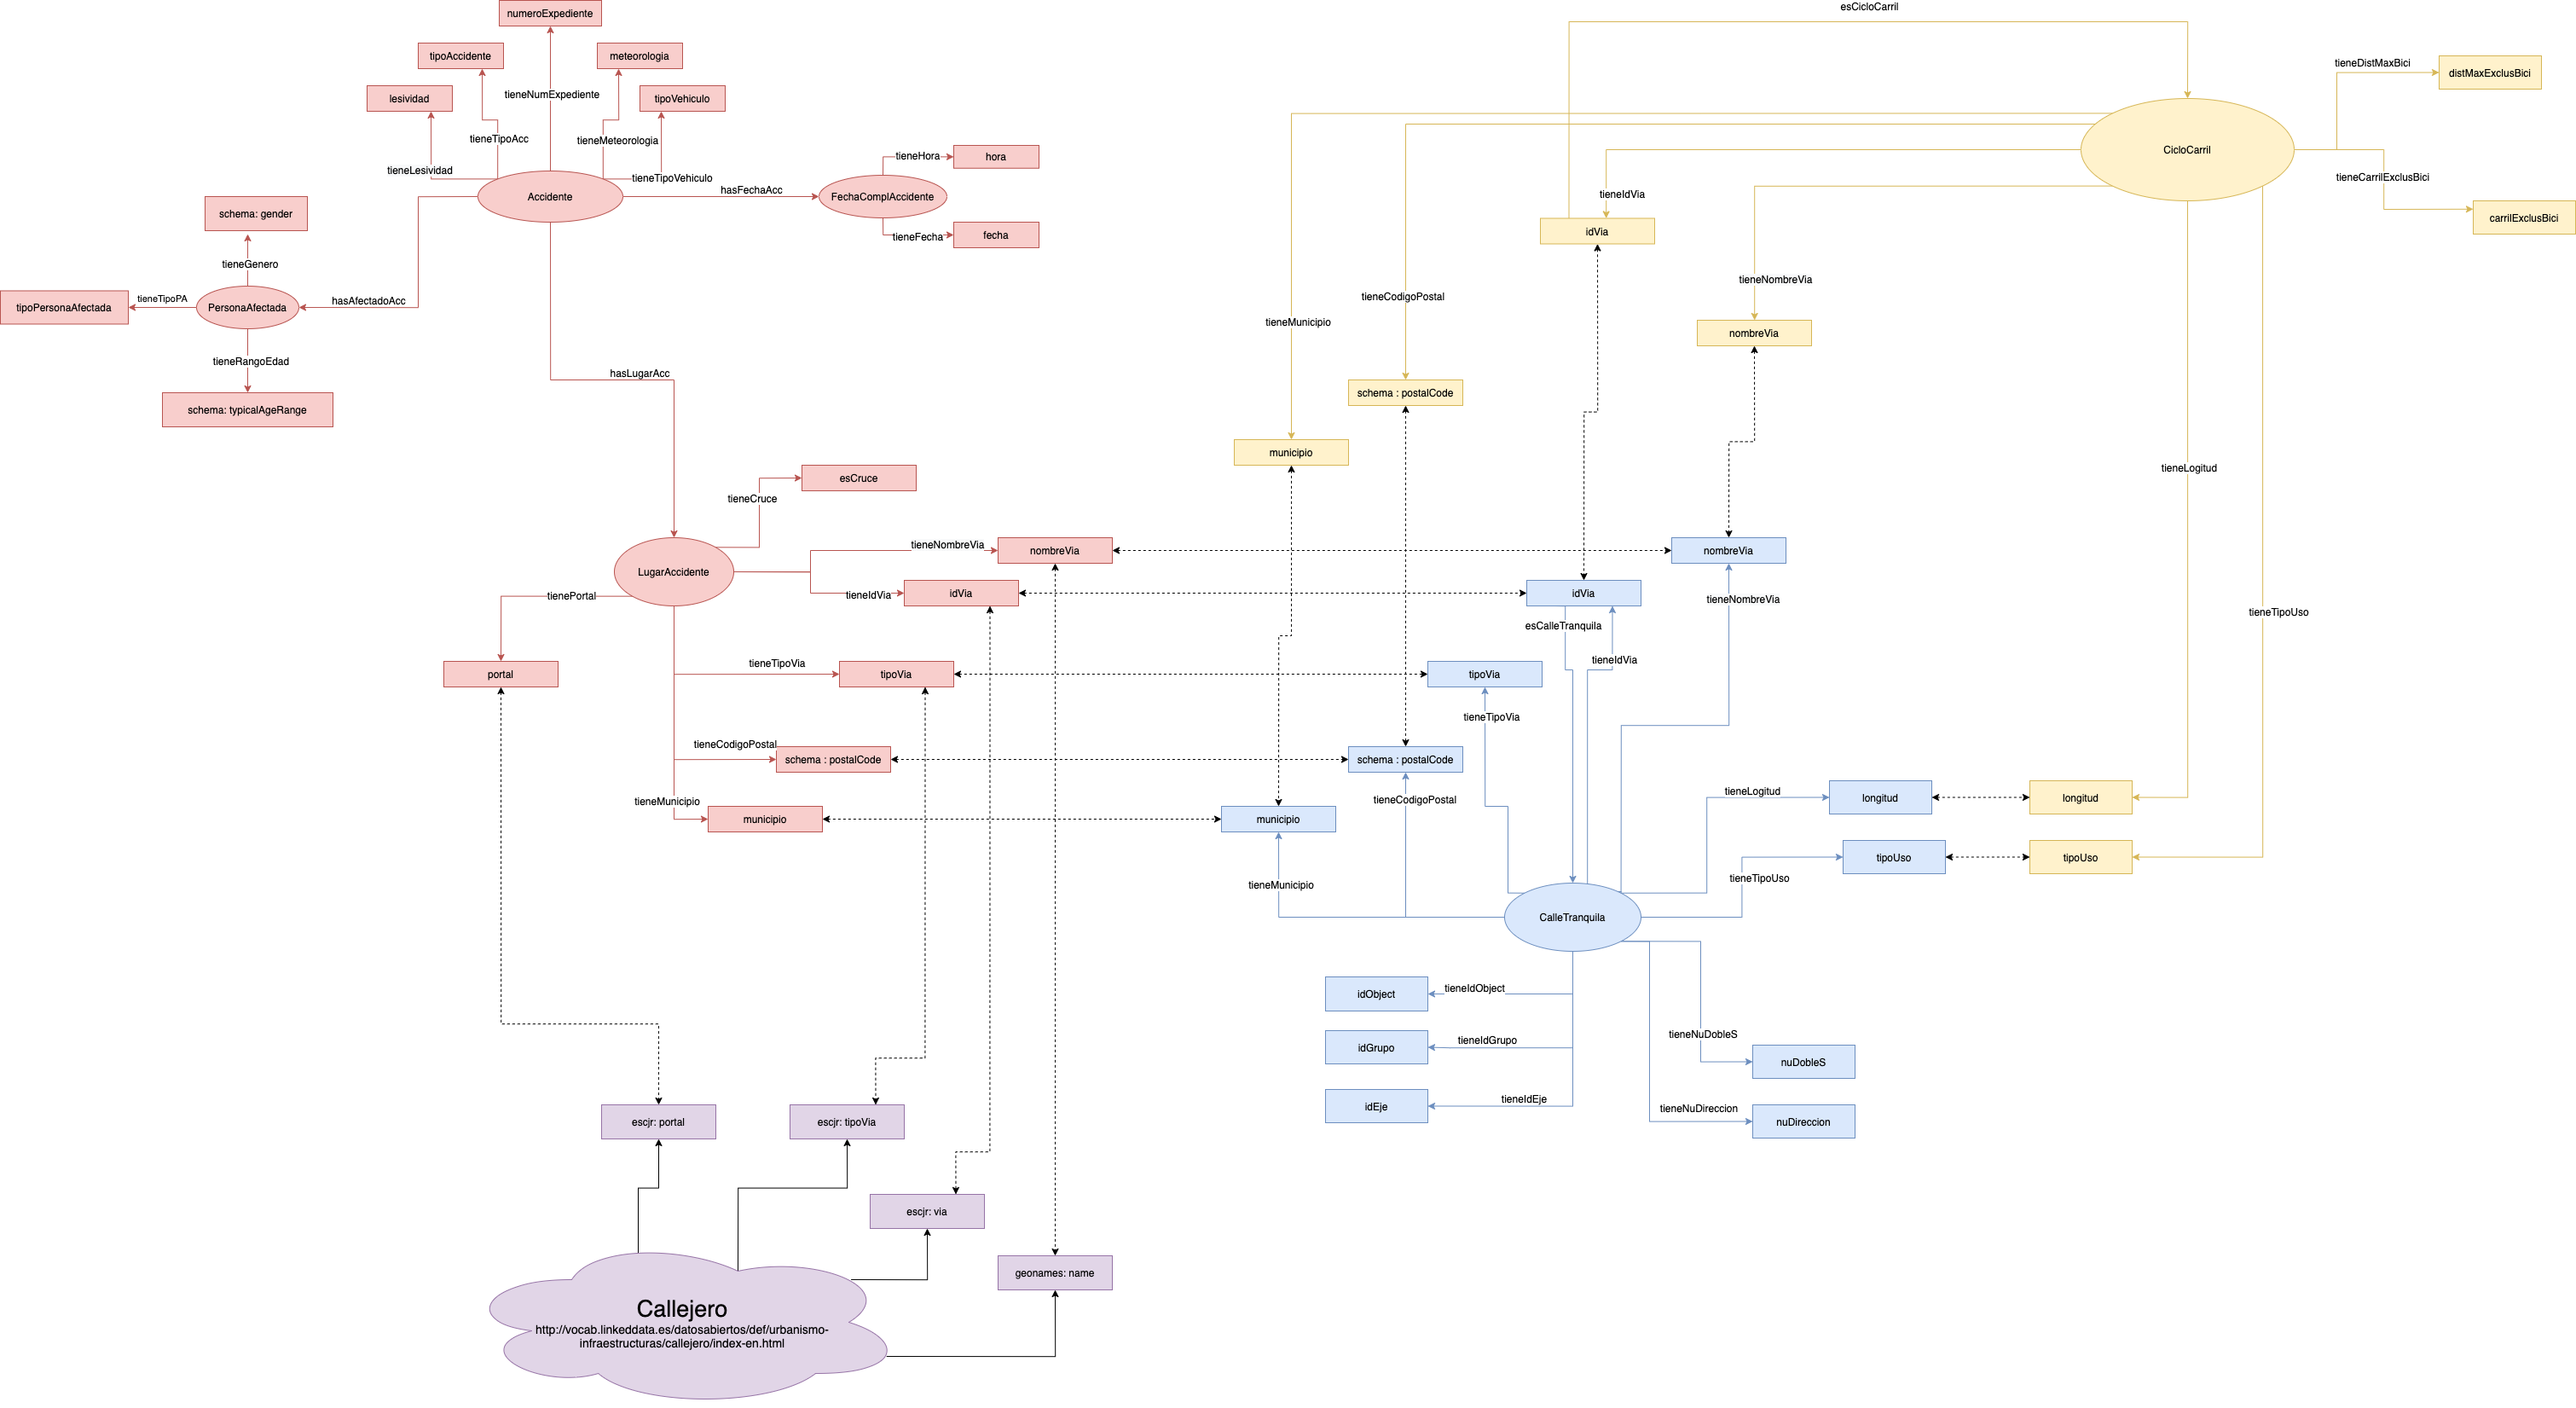
\includegraphics[angle=90, width=0.8\textwidth]{images/diagramaAppTotal.png} 
  \\
  \caption{Diagrama de los datos enlazados en la Aplicación}
  \label{fig:esquemaTotalVocab}
\end{figure}


%%---------------------------------------------------------

\chapter{Definición de Vocabularios}

En este proyecto se han definido 2 vocabularios y se ha realizado una propuesta de modificación para el Callejero \cite{ciudadesbiertas_callejero}. Para ello se han reutilizado elementos de otras ontologías y se han generado nuevas clases y propiedades que han permitido representar de forma clara y detallada los nuevos elementos propuestos.


Se han tomado en cuenta los datasets proporcionados por el Ayuntamiento de Madrid \cite{datosabiertos_ayuntmadrid} para ello y se han definido acorde con los datos que se estaban proporcionando en los mismos. De esta forma se ha pretendido seguir la linea marcada por la institución para la publicación de los mismos con la intención de interferir lo mínimo en el proceso de creación ya definido.


Como norma general los vocabularios han de seguir un proceso de coordinación entre instituciones y deben realizarse mediante consenso entre desarrolladores y entidades proveedoras de los mismos. Para este proyecto no ha sido posible dicho estudio exhaustivo sobre cada una de las propiedades y clases, es por ello que se ha intentado asemejar lo máximo a los valores proporcionados por el Ayuntamiento de Madrid y se han realizado las propuestas a la plataforma ciudadesabiertas \cite{ciudadesabiertas_catalogoVocabs}.



%----------------------------------------------------------------------------------------------------------------------------------------------------------------------------------------------------------------------------------------------
\clearpage
\section{Vocabulario de Accidentes de Bicicletas}

Para el vocabulario asociado con los accidentes de bicicletas se han tomado como referencia los datos proporcionados por el ayuntamiento de Madrid.  \cite{datosMadrid_accidentesDeBicicleta}. En estos datasets se muestran los accidentes de tráfico con implicación de bicicletas dentro de la jurisdicción del ayuntamiento.
\newline
Se han añadido además algunos datos no proporcionados en estos datasets, como es el Municipio, el id de la vía u otros, ya que se han considerado necesarios para la definición de un vocabulario reutilizable y aplicable a otros datasets.
\newline
Este vocabulario se ha definido con el objetivo de ser válido tanto para accidentes de tráfico de bicicletas como de automóviles u otros vehículos. Aun habiendo partido de un dataset en el que se representaban los accidentes relativos al primer caso, todos los elementos definidos pueden ser utilizados en cualquier tipo de accidente. Debido a que este trabajo está enfocado a crear una aplicación para la seguridad de bicicletas, se ha partido de esta base, pero podría ser perfectamente reutilizado para otro tipo de accidente añadiéndole propiedades necesarias para los mismos como podrían ser la velocidad, el numero de pasajeros...
\newline
La organización del conjunto de datos se hará siguiendo el diagrama \ref{fig:diagramaOntologAccid}

\begin{figure}[h]
	\centering
	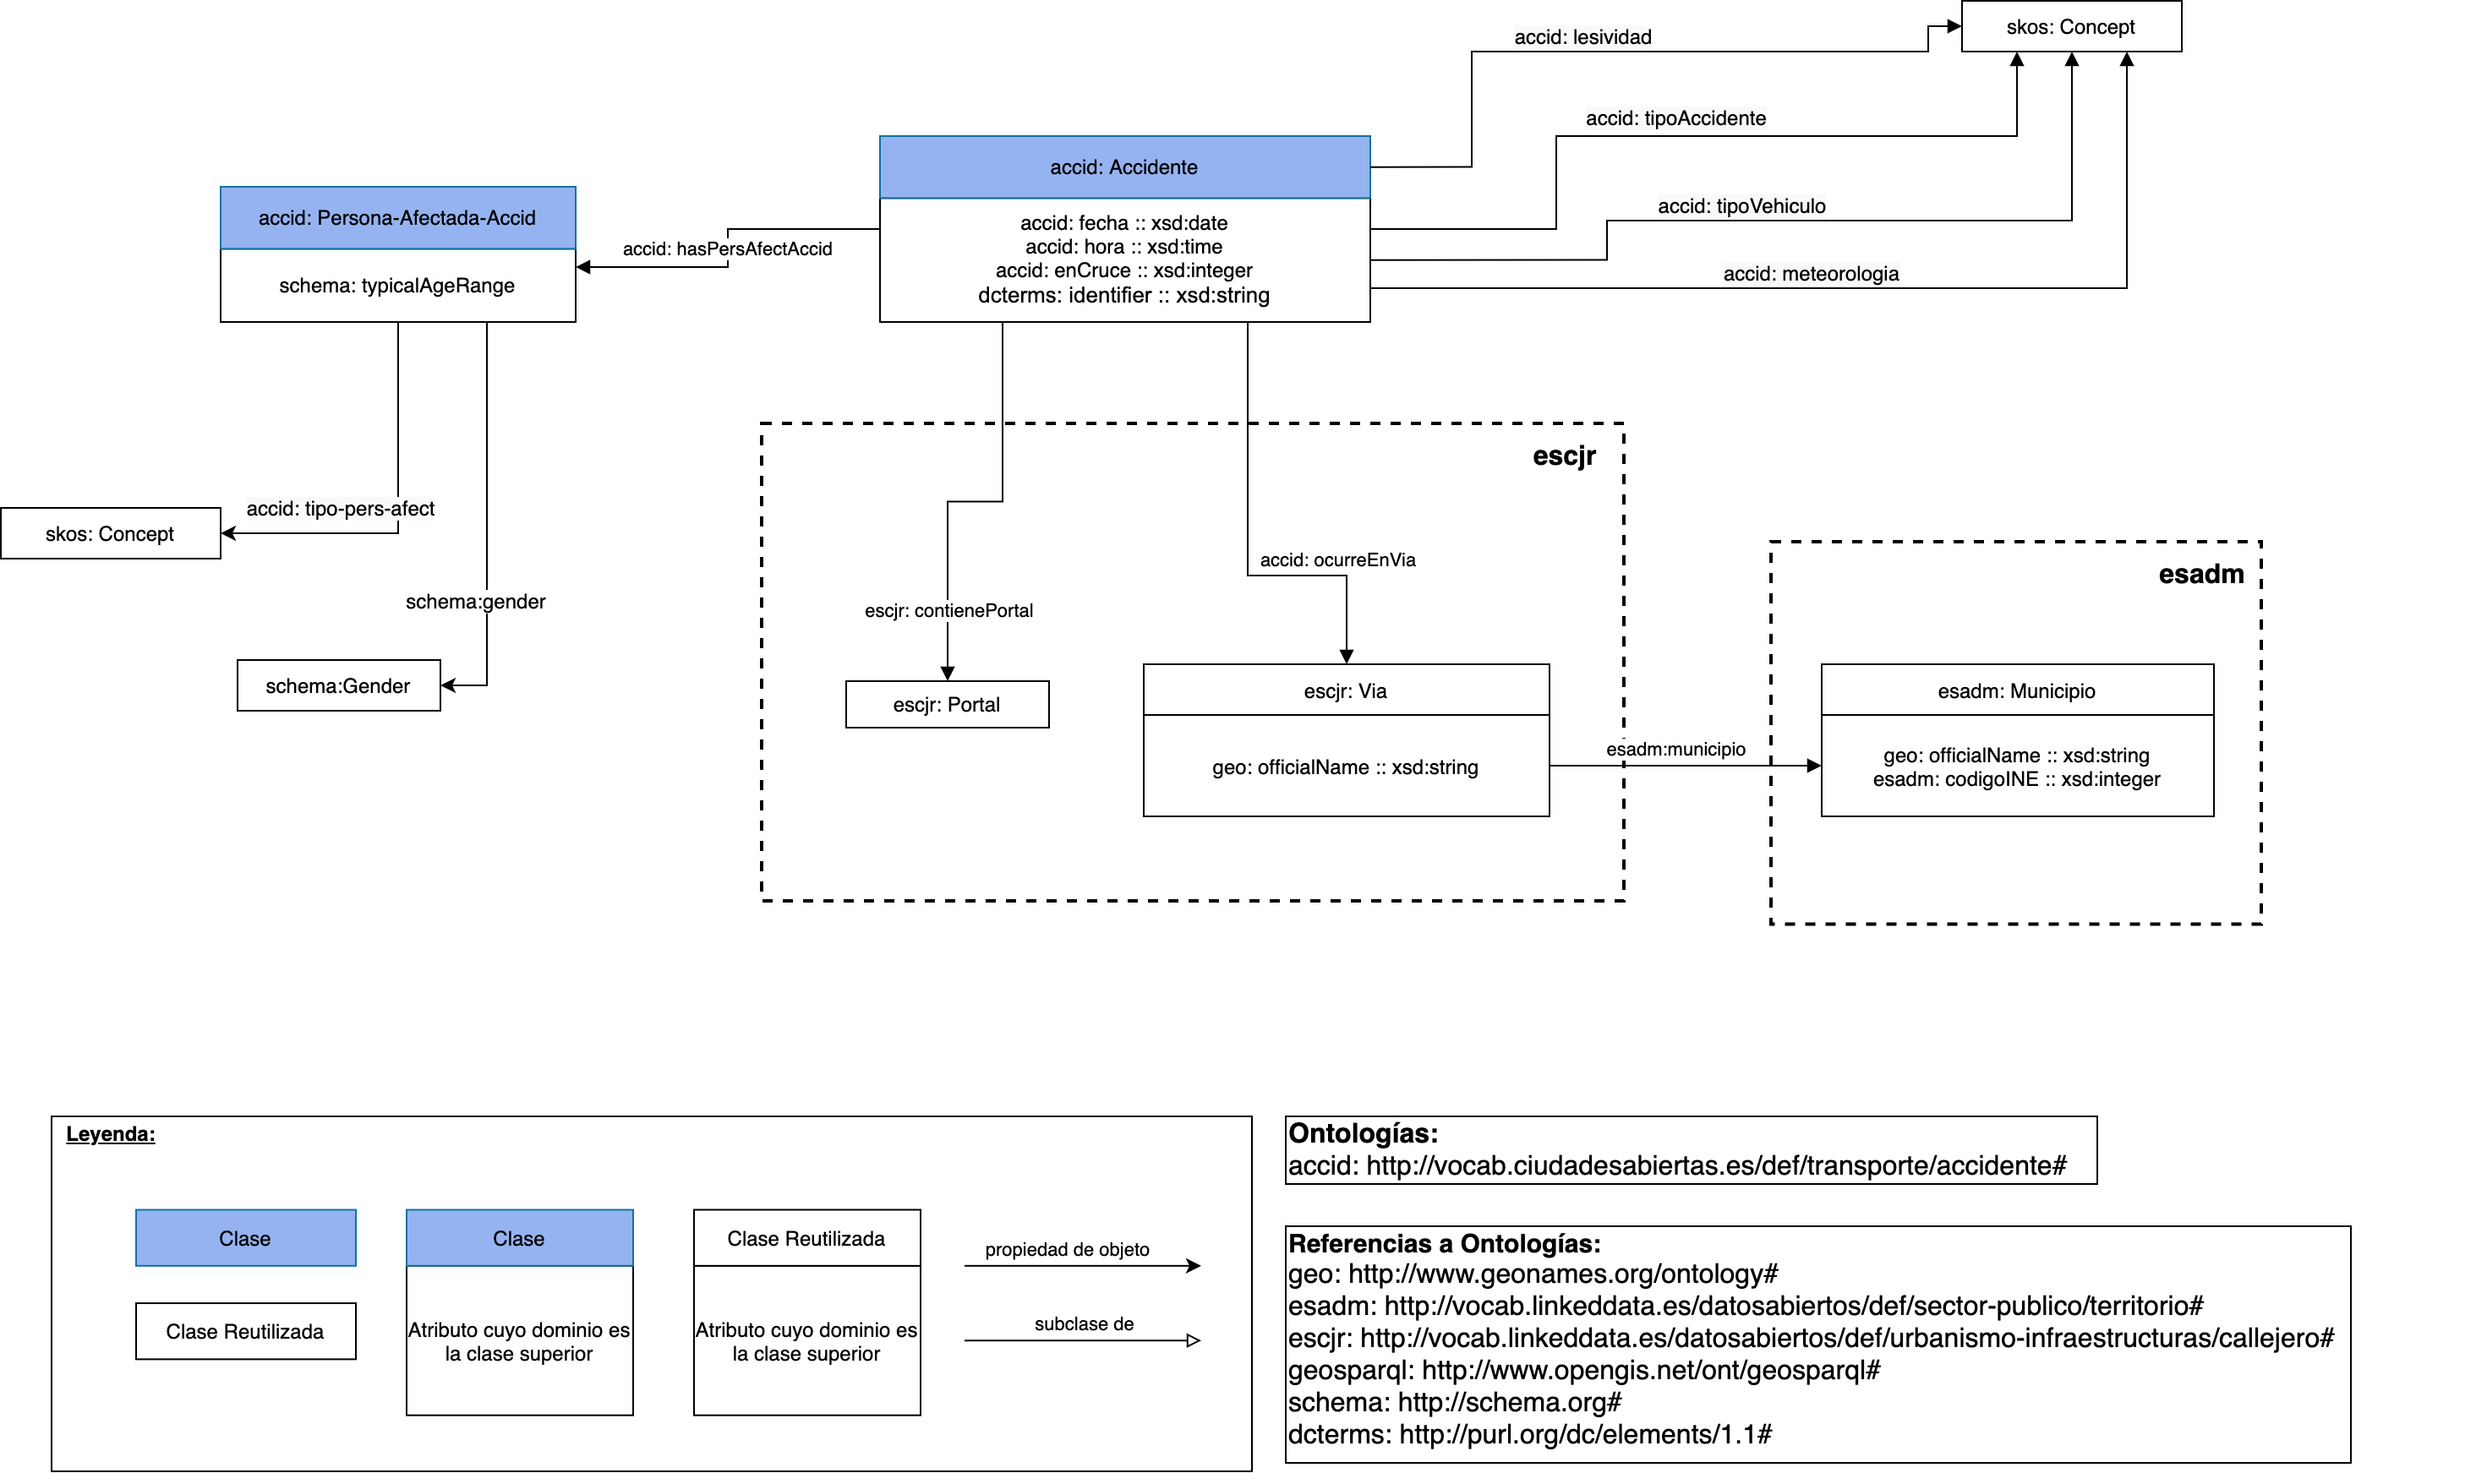
\includegraphics[angle=0, width=1\textwidth]{images/diagramaAccidBici.png}  
	
	\caption{Diagrama de Ontología de Accidentes.}
	\label{fig:diagramaOntologAccid}
\end{figure}


Para la representación de los datos de accidentes de trafico se han definido varias clases y propiedades. Se han reutilizado elementos ya definidos en el vocabulario de Callejero \cite{ciudadesbiertas_callejero}, de Territorio \cite{datoabiertos_municipio} y de Schema \cite{schema_org}.

\clearpage
En la siguiente tabla se muestran los Namespaces usados.

\begin{figure}[h]
	\centering
		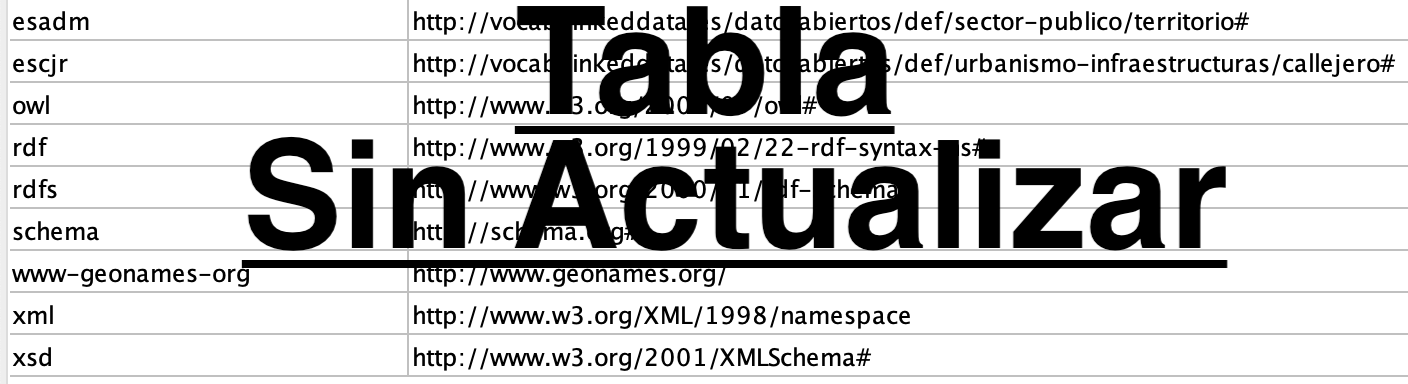
\includegraphics[angle=0, width=0.8\textwidth]{images/tablaIRIsAccidentesBici.png}  
	\caption{Namespaces usados para Accidentes}
\end{figure}




Se ha optado por mantener la separación de elementos como fecha y hora, calle y numero debido a que en la fuente de origen están así dispuestos y en la posterior aplicación final que se va a construir será más conveniente tener esa información por separado, para poder disponer de datos a horas con menos luminosidad o calles completas(sin conocer la posición exacta), por ejemplo.


Para este conjunto de datos se ha optado por añadir, además de los ya proporcionados por la fuente de origen del ayuntamiento, nueva información como la propiedad ``esCruce``, el municipio, el tipo de vía o el identificador de vía. Son propiedades inferidas de la información proporcionada que permiten que sea más sencillo su tratamiento y uso, para esta u otras aplicaciones que puedan tener estos datos.
EsCruce se obtendrá del nombre de la calle, del cual atendiendo a varios patrones se puede determinar si el accidente ha ocurrido en una intersección de dos o más vías.
El Municipio se ha añadido para su posible reutilización posterior utilizando otros datasets de otras localidades, para este caso será siempre Madrid.
El Identificador de Vía se obtendrá comparando el nombre de la vía y su tipo con el Callejero de Madrid, el cual proporcionará este valor único que represente la vía.
El tipo de vía finalmente se ha eliminado del vocabulario ya que no tiene relevancia para los datos obtenidos de éste, más allá de la obtención del identificador de vía. En cualquier caso, si fuese necesario se podría obtener a partir del nombre de la calle, aunque no se ha considerado relevante para añadirlo a la ontología.

En este conjunto de datos se ha hecho un cambio relevante con respecto al original y que será detallada en el capítulo Transformaciones en los vocabularios. Los accidentes que han ocurrido entre un cruce de vías se han separado en tantos registros como vías interfieran. De este modo será mucho más simple la búsqueda de accidentes ocurridos en una calle y se podrá hacer una búsqueda más sencilla de ellas. Se podrá identificar si dos o más registros pertenecen al mismo accidente por el número de expediente, el cual se conserva igual en ambos.





\clearpage
\subsection{Clases}



\begin{mybox}{Accidente}
\begin{flushleft}
\underline{\textbf{IRI:}}

\url{http://vocab.ciudadesabiertas.es/def/accidente/accid-bici#Accidente}
\newline

Siniestro ocurrido con implicación de bicicletas.
\newline

\underline{\textbf{Definida por:}}
\url{http://vocab.ciudadesabiertas.es/def/accidente/accid-bici}
\newline


\underline{\textbf{En dominio de:}}
\newline PersonaAfectada, \hspace{2em} LugarAccidente,	\hspace{2em}meteorología,
\newline lesividad,	\hspace{2em}tipoVehiculo,	\hspace{2em}tipoAccidente,
\newline numeroExpediente
	
\underline{\textbf{Tiene Superclases:}}
\newline fecha, \hspace{2em} time



\end{flushleft}
\end{mybox}

%----------------------------------------------------------------------------------------------------------------------------------------------------------------------------------------------------------------------------------------------

\begin{mybox}{PersonaAfectada}
\begin{flushleft}
\underline{\textbf{IRI:}}

\url{http://vocab.ciudadesabiertas.es/def/accidente/accid-bici#PersonaAfectada}
\newline

La persona perjudicada por el accidente de tráfico.
\newline

\underline{\textbf{Definida por:}}

\url{http://vocab.ciudadesabiertas.es/def/accidente/accid-bici}
\newline

\underline{\textbf{Subclase de:}}
\newline Accidente
\newline

\underline{\textbf{En dominio de:}}
\newline tipoPersonaAfectada, \hspace{2em} gender, \hspace{2em} typicalAgeRange

\end{flushleft}
\end{mybox}
%----------------------------------------------------------------------------------------------------------------------------------------------------------------------------------------------------------------------------------------------


\begin{mybox}{LugarAccidente}
\begin{flushleft}
\underline{\textbf{IRI:}}
\url{http://vocab.ciudadesabiertas.es/def/accidente/accid-bici#LugarAccidente}
\newline

El momento en el que ocurrió el siniestro.
\newline

\underline{\textbf{Definida por:}}
\url{http://vocab.ciudadesabiertas.es/def/accidente/accid-bici}
\newline

\underline{\textbf{Subclase de:}}
\newline Accidente
\newline

\underline{\textbf{En dominio de:}}
\newline esCruce, \hspace{2em} municipio, \hspace{2em} Calle

\end{flushleft}
\end{mybox}
%----------------------------------------------------------------------------------------------------------------------------------------------------------------------------------------------------------------------------------------------


\begin{mybox}{Calle}
\begin{flushleft}
\underline{\textbf{IRI:}}
\url{http://vocab.ciudadesabiertas.es/def/accidente/accid-bici#Calle}
\newline

Representación de una via de una ciudad.
\newline

\underline{\textbf{Definida por:}}
\url{http://vocab.ciudadesabiertas.es/def/accidente/accid-bici}
\newline

\underline{\textbf{Tiene subclase:}}
\newline tipoVia,\hspace{2em} Via,\hspace{2em} portal
\newline 

\underline{\textbf{Tiene Superclases:}}
\newline LugarAccidente \hspace{2em} nombre oficial

\end{flushleft}
\end{mybox}

%----------------------------------------------------------------------------------------------------------------------------------------------------------------------------------------------------------------------------------------------



\begin{mybox}{Portal}
\begin{flushleft}
\underline{\textbf{IRI:}}
\url{http://vocab.linkeddata.es/datosabiertos/def/urbanismo-infraestructuras/callejero#Portal}
\newline

Ha sido definido por la plataforma ciudadesabiertas \cite{datosabiertos_portal}.
Subacceso independiente exterior (al aire libre) a una misma construcción. Para una misma construcción, con un mismo número de vía, pueden existir varias entradas que pueden estar numeradas con números o letras. [fuente: Modelo de Direcciones de la Administración General del Estado v.2]
\newline

\underline{\textbf{Definida por:}}
\url{http://vocab.linkeddata.es/datosabiertos/def/urbanismo-infraestructuras/callejero}
\newline

\underline{\textbf{Tiene Superclases:}}
	LugarAccidente
\newline

\end{flushleft}
\end{mybox}
%----------------------------------------------------------------------------------------------------------------------------------------------------------------------------------------------------------------------------------------------



\begin{mybox}{municipio}
\begin{flushleft}
\underline{\textbf{IRI:}}
\url{http://vocab.linkeddata.es/datosabiertos/def/sector-publico/territorio#Municipio}
\newline

Se ha reutilizado la definición de Municipio proporcionada por vocab.linkeddata.es \cite{datoabiertos_municipio}
Un Municipio es el ente local definido en el artículo 140 de la Constitución española y la entidad básica de la organización territorial del Estado según el artículo 1 de la Ley 7/1985, de 2 de abril, Reguladora de las Bases del Régimen Local. Tiene personalidad jurídica y plena capacidad para el cumplimiento de sus fines. La delimitación territorial de Municipio está recogida del REgistro Central de Cartografía del IGN. Su nombre, que se especifica con la propiedad dct:title, es el proporcionado por el Registro de Entidades Locales del Ministerio de Política Territorial, en \url{http://www.ine.es/nomen2/index.do}
\newline


\underline{\textbf{Definida por:}}
\url{http://purl.org/derecho/vocabulario}
\url{http://vocab.linkeddata.es/datosabiertos/def/sector-publico/territorio}
\url{http://www.ign.es/ign/resources/acercaDe/tablon/ModeloDireccionesAGE}
\newline

\underline{\textbf{Tiene Superclases:}}
\newline LugarAccidente



\end{flushleft}
\end{mybox}
%----------------------------------------------------------------------------------------------------------------------------------------------------------------------------------------------------------------------------------------------




\begin{mybox}{Via}
\begin{flushleft}
\underline{\textbf{IRI:}}
\url{http://vocab.linkeddata.es/datosabiertos/def/urbanismo-infraestructuras/callejero#Via}
\newline

Se ha reutilizado la definición de Municipio proporcionada por vocab.linkeddata.es \cite{datoabiertos_idVia}

Vía de comunicación construida para la circulación. En su definición según el modelo de direcciones de la Administración General del Estado, Incluye calles, carreteras de todo tipo, caminos, vías de agua, pantalanes, etc. Asimismo, incluye la pseudovía., es decir todo aquello que complementa o sustituye a la vía. En nuestro caso, este término se utiliza para hacer referencia a las vías urbanas.
Representación numérica de la misma.
\newline

\underline{\textbf{Definida por:}}
\url{http://vocab.linkeddata.es/datosabiertos/def/urbanismo-infraestructuras/callejero}
\newline

\underline{\textbf{Tiene Superclases:}}
\newline Calle





\end{flushleft}
\end{mybox}
%----------------------------------------------------------------------------------------------------------------------------------------------------------------------------------------------------------------------------------------------




\begin{mybox}{numeroExpediente}
\begin{flushleft}
\underline{\textbf{IRI:}}
\url{http://vocab.ciudadesabiertas.es/def/accidente/accid-bici#numeroExpediente}
\newline

El identificador del siniestro que proporciona el ayuntamiento.
\newline

\underline{\textbf{Definida por:}}
\newline \url{http://vocab.ciudadesabiertas.es/def/accidente/accid-bici}
\newline

\underline{\textbf{Tiene Superclases:}}
\newline Accidente
\newline


\end{flushleft}
\end{mybox}
%----------------------------------------------------------------------------------------------------------------------------------------------------------------------------------------------------------------------------------------------


%----------------------------------------------------------------------------------------------------------------------------------------------------------------------------------------------------------------------------------------------
%----------------------------------------------------------------------------------------------------------------------------------------------------------------------------------------------------------------------------------------------
%----------------------------------------------------------------------------------------------------------------------------------------------------------------------------------------------------------------------------------------------
%----------------------------------------------------------------------------------------------------------------------------------------------------------------------------------------------------------------------------------------------



\clearpage
\subsection{Propiedades de datos}
%----------------------------------------------------------------------------------------------------------------------------------------------------------------------------------------------------------------------------------------------
%----------------------------------------------------------------------------------------------------------------------------------------------------------------------------------------------------------------------------------------------
%----------------------------------------------------------------------------------------------------------------------------------------------------------------------------------------------------------------------------------------------
%----------------------------------------------------------------------------------------------------------------------------------------------------------------------------------------------------------------------------------------------



\begin{mybox}{fecha}
\begin{flushleft}
\underline{\textbf{IRI:}}
\url{http://vocab.ciudadesabiertas.es/def/transporte/accidente#fecha}
\newline

Fecha en la que ocurre el siniestro. Dia, mes y año, sin incluir la hora del accidente.
\newline

\underline{\textbf{Definida por:}}\newline
\url{http://vocab.ciudadesabiertas.es/def/transporte/accidente}
\newline

\underline{\textbf{Dominio:}} Accidente
\newline

\underline{\textbf{Rango:}}  xsd:date
\newline

\end{flushleft}
\end{mybox}
%----------------------------------------------------------------------------------------------------------------------------------------------------------------------------------------------------------------------------------------------



\begin{mybox}{hora}
\begin{flushleft}
\underline{\textbf{IRI:}}
\url{http://vocab.ciudadesabiertas.es/def/transporte/accidente#hora}
\newline

Hora en la que ocurre el siniestro.
\newline

\underline{\textbf{Definida por:}}\newline
\url{http://vocab.ciudadesabiertas.es/def/transporte/accidente}
\newline

\underline{\textbf{Dominio:}}  Accidente
\newline

\underline{\textbf{Rango:}}  xsd:time
\newline

\end{flushleft}
\end{mybox}
%----------------------------------------------------------------------------------------------------------------------------------------------------------------------------------------------------------------------------------------------



\begin{mybox}{officialName}
\begin{flushleft}
\underline{\textbf{IRI:}}
\url{http://www.geonames.org/ontology#officialName}
\newline

Definición reutilizada del Callejero de DatosAbiertos \cite{ciudadesbiertas_callejero}.
\\Un nombre en el idioma oficial local.
\newline


\underline{\textbf{Definida por:}}\newline
\url{http://www.geonames.org/ontology}
\newline

\underline{\textbf{Dominio:}}	Via
\newline

\underline{\textbf{Rango:}}  xsd:string
\newline

\end{flushleft}
\end{mybox}
%----------------------------------------------------------------------------------------------------------------------------------------------------------------------------------------------------------------------------------------------




\begin{mybox}{typicalAgeRange}
\begin{flushleft}
\underline{\textbf{IRI:}}
\url{https://schema.org/typicalAgeRange}
\newline

Rango de edad en el que se encuentra la persona afectada.
\newline Seguirá el siguiente formato definido por Schema.org: 
\newline  %\textcolor{red}{ 
$<$span property="typicalAgeRange"$>$10-12</span$>$  \cite{schema_typicalAgeRange}
\newline

\underline{\textbf{Definida por:}}\newline
\url{https://schema.org/typicalAgeRange}
\newline

\underline{\textbf{Dominio:}}  PersonaAfectada
\newline

\underline{\textbf{Rango:}} xsd:string
\newline

\end{flushleft}
\end{mybox}
%----------------------------------------------------------------------------------------------------------------------------------------------------------------------------------------------------------------------------------------------










\begin{mybox}{enCruce}
\begin{flushleft}
\underline{\textbf{IRI:}}
\url{http://vocab.ciudadesabiertas.es/def/transporte/accidente#enCruce}
\newline

Si el accidente ocurrió en un cruce entre 2 o más vías.
\\Está representado como un integer ya que puede ser un cruce de múltiples calles. En caso de ser un valor booleano solo podria representarse la intersección entre calles. Esta propiedad representa el numero de calles asociadas. En caso de que no fuese cruce se le asignaria el valor 0, en los casos en los que si se asignaria 2, 3 o números sucesivos dependiendo del numero de calles de la intersección.
\newline

\underline{\textbf{Definida por:}}\newline
\url{http://vocab.ciudadesabiertas.es/def/transporte/accidente}
\newline

\underline{\textbf{Dominio:}} 	Accidente
\newline

\underline{\textbf{Rango:}} 	xsd:integer
\newline

\end{flushleft}
\end{mybox}
%----------------------------------------------------------------------------------------------------------------------------------------------------------------------------------------------------------------------------------------------








\begin{mybox}{identifier}
\begin{flushleft}
\underline{\textbf{IRI:}}
\url{http://purl.org/dc/terms/identifier}
\newline

An unambiguous reference to the resource within a given context.
\\Recommended practice is to identify the resource by means of a string conforming to an identification system. Examples include International Standard Book Number (ISBN), Digital Object Identifier (DOI), and Uniform Resource Name (URN). Persistent identifiers should be provided as HTTP URIs \cite{dc_identifier}.
\newline

\underline{\textbf{Definida por:}}\newline
\url{http://purl.org/dc/elements}
\newline

\underline{\textbf{Dominio:}} 	Accidente
\newline

\underline{\textbf{Rango:}}\newline
	http://www.w3.org/2000/01/rdf-schema\#Literal
\newline

\end{flushleft}
\end{mybox}
%----------------------------------------------------------------------------------------------------------------------------------------------------------------------------------------------------------------------------------------------






\begin{mybox}{codigoINE}
\begin{flushleft}
\underline{\textbf{IRI:}}
\url{http://vocab.linkeddata.es/datosabiertos/def/sector-publico/territorio#codigoINE}
\newline

Indicador de si las bicicletas disponen o no de un carril propio para su circulación.
\newline


\underline{\textbf{Definida por:}}\newline
\url{http://vocab.linkeddata.es/datosabiertos/def/sector-publico/territorio}
\newline

\underline{\textbf{Dominio:}}
	Municipio
\newline

\underline{\textbf{Rango:}}
	xsd:integer
\newline

\end{flushleft}
\end{mybox}
%----------------------------------------------------------------------------------------------------------------------------------------------------------------------------------------------------------------------------------------------



























\clearpage
\subsection{Propiedades de objeto}
%----------------------------------------------------------------------------------------------------------------------------------------------------------------------------------------------------------------------------------------------
%----------------------------------------------------------------------------------------------------------------------------------------------------------------------------------------------------------------------------------------------
%----------------------------------------------------------------------------------------------------------------------------------------------------------------------------------------------------------------------------------------------
%----------------------------------------------------------------------------------------------------------------------------------------------------------------------------------------------------------------------------------------------




\begin{mybox}{hasPersonaAfectada}
\begin{flushleft}
\underline{\textbf{IRI:}}
\url{http://vocab.ciudadesabiertas.es/def/transporte/accidente#hasPersonaAfectada}
\newline

Persona que se asocia a un accidente. Esta a su vez puede tener más características como por ejemplo el rol que tuvo (peatón, conductor), edad y género.
\newline

\underline{\textbf{Definida por:}}
\newline \url{http://vocab.ciudadesabiertas.es/def/transporte/accidente}
\newline

\underline{\textbf{Dominio:}} 	
\newline Accidente
\newline

\underline{\textbf{Rango:}} 
\newline PersonaAfectada

\end{flushleft}
\end{mybox}
%----------------------------------------------------------------------------------------------------------------------------------------------------------------------------------------------------------------------------------------------




\begin{mybox}{tipoVehiculo}
\begin{flushleft}
\underline{\textbf{IRI:}}
\url{http://vocab.ciudadesabiertas.es/def/transporte/accidente#tipoVehiculo}
\newline

Tipo de vehículo afectado, p.ej. Bicicleta, Bicicleta EPAC (pedaleo asistido). Se han definido los siguientes elementos:
\newline \url{http://vocab.linkeddata.es/datosabiertos/kos/transporte/accidente/tipo-vehiculo/BICICLETA}
\newline \url{http://vocab.linkeddata.es/datosabiertos/kos/transporte/accidente/tipo-vehiculo/BICICLETA-EPAC}
\newline

\underline{\textbf{Definida por:}}\newline
\url{http://vocab.ciudadesabiertas.es/def/transporte/accidente}
\newline

\underline{\textbf{Dominio:}} Accidente
\newline

\underline{\textbf{Rango:}} concept
\newline

\end{flushleft}
\end{mybox}
%----------------------------------------------------------------------------------------------------------------------------------------------------------------------------------------------------------------------------------------------



\begin{mybox}{meteorologia}
\begin{flushleft}
\underline{\textbf{IRI:}}
\url{http://vocab.ciudadesabiertas.es/def/transporte/accidente#meteorologia}
\newline

Condiciones ambientales que se dan en el momento del siniestro. Se han definido varios tipos posibles:
\newline \url{http://vocab.linkeddata.es/datosabiertos/kos/transporte/accidente/meteorologia/DESPEJADO}
\newline \url{http://vocab.linkeddata.es/datosabiertos/kos/transporte/accidente/meteorologia/LLUVIA-DEBIL}
\newline \url{http://vocab.linkeddata.es/datosabiertos/kos/transporte/accidente/meteorologia/LLUVIA-INTENSA}
\newline \url{http://vocab.linkeddata.es/datosabiertos/kos/transporte/accidente/meteorologia/NUBLADO}
\newline \url{http://vocab.linkeddata.es/datosabiertos/kos/transporte/accidente/meteorologia/GRANIZANDO}
\newline \url{http://vocab.linkeddata.es/datosabiertos/kos/transporte/accidente/meteorologia/DESCONOCIDO}
\newline

\underline{\textbf{Definida por:}}\newline
\url{http://vocab.ciudadesabiertas.es/def/transporte/accidente}
\newline

\underline{\textbf{Dominio:}}  Accidente
\newline

\underline{\textbf{Rango:}} concept
\newline

\end{flushleft}
\end{mybox}
%----------------------------------------------------------------------------------------------------------------------------------------------------------------------------------------------------------------------------------------------


\begin{mybox}{tipoAccidente}
\begin{flushleft}
\underline{\textbf{IRI:}}
\url{http://vocab.ciudadesabiertas.es/def/transporte/accidente#tipoAccidente}
\newline

Tipo de accidente asociado. Se han definido para ello varios tipos posibles:
\newline \url{http://vocab.linkeddata.es/datosabiertos/kos/transporte/accidente/tipo-accidente/COLISION}
\newline \url{http://vocab.linkeddata.es/datosabiertos/kos/transporte/accidente/tipo-accidente/COLISION-DOBLE}
\newline \url{http://vocab.linkeddata.es/datosabiertos/kos/transporte/accidente/tipo-accidente/COLISION-MULTIPLE}
\newline \url{http://vocab.linkeddata.es/datosabiertos/kos/transporte/accidente/tipo-accidente/ALCANCE}
\newline \url{http://vocab.linkeddata.es/datosabiertos/kos/transporte/accidente/tipo-accidente/CHOQUE-NO-VEHICULO}
\newline \url{http://vocab.linkeddata.es/datosabiertos/kos/transporte/accidente/tipo-accidente/ATROPELLO-PEATON}
\newline \url{http://vocab.linkeddata.es/datosabiertos/kos/transporte/accidente/tipo-accidente/VUELCO}
\newline \url{http://vocab.linkeddata.es/datosabiertos/kos/transporte/accidente/tipo-accidente/CAIDA}
\newline \url{http://vocab.linkeddata.es/datosabiertos/kos/transporte/accidente/tipo-accidente/OTROS}
\newline

\underline{\textbf{Definida por:}}
\newline \url{http://vocab.ciudadesabiertas.es/def/transporte/accidente}
\newline

\underline{\textbf{Dominio:}}  Accidente
\newline

\underline{\textbf{Rango:}}  concept
\newline

\end{flushleft}
\end{mybox}
%----------------------------------------------------------------------------------------------------------------------------------------------------------------------------------------------------------------------------------------------




\begin{mybox}{lesividad}
\begin{flushleft}
\underline{\textbf{IRI:}}
\url{http://vocab.ciudadesabiertas.es/def/transporte/accidente#lesividad}
\newline

Código que indica la gravedad del siniestro para la persona afectada.
\newline

Para su uso se han definido los siguientes elementos:
\newline 01 Atencion en urgencias sin posterior ingreso. - LEVE:
\newline \url{http://vocab.linkeddata.es/datosabiertos/kos/transporte/accidente/lesividad/01}
\newline 02 Ingreso inferior o igual a 24 horas - LEVE:
\newline \url{http://vocab.linkeddata.es/datosabiertos/kos/transporte/accidente/lesividad/02}
\newline 03 Ingreso superior a 24 horas. - GRAVE:
\newline \url{http://vocab.linkeddata.es/datosabiertos/kos/transporte/accidente/lesividad/03}
\newline 04 Fallecido 24 horas - FALLECIDO:
\newline \url{http://vocab.linkeddata.es/datosabiertos/kos/transporte/accidente/lesividad/04}
\newline 05 Asistencia sanitaria ambulatoria con posterioridad - LEVE:
\newline \url{http://vocab.linkeddata.es/datosabiertos/kos/transporte/accidente/lesividad/05}
\newline 06 Asistencia sanitaria inmediata en centro de salud o mutua - LEVE:
\newline \url{http://vocab.linkeddata.es/datosabiertos/kos/transporte/accidente/lesividad/06}
\newline 07 Asistencia sanitaria solo en el lugar del accidente - LEVE:
\newline \url{http://vocab.linkeddata.es/datosabiertos/kos/transporte/accidente/lesividad/07}
\newline 14 Sin asistencia sanitaria:
\newline \url{http://vocab.linkeddata.es/datosabiertos/kos/transporte/accidente/lesividad/14}
\newline 77 Se desconoce:
\newline \url{http://vocab.linkeddata.es/datosabiertos/kos/transporte/accidente/lesividad/77}
\newline


\underline{\textbf{Definida por:}}
\newline \url{http://vocab.ciudadesabiertas.es/def/transporte/accidente}
\newline

\underline{\textbf{Dominio:}}  Accidente
\newline

\underline{\textbf{Rango:}} concept
\newline

\end{flushleft}
\end{mybox}
%----------------------------------------------------------------------------------------------------------------------------------------------------------------------------------------------------------------------------------------------






\begin{mybox}{gender}
\begin{flushleft}
\underline{\textbf{IRI:}}
\url{https://schema.org/gender}
\newline

Género de la persona afectada.
\newline Seguirá el formato definido por Schema.org \cite{schema_gender}
Se utilizarán las siguientes definidas en la clase:
\newline \url{http://schema.org/Male}
\newline \url{http://schema.org/Female}
\newline \url{http://schema.org/Mixed}
\newline

\underline{\textbf{Definida por:}}\newline
\url{https://schema.org/gender}
\newline

\underline{\textbf{Dominio:}} PersonaAfectada
\newline

\underline{\textbf{Rango:}} Gender \cite{schema_gender_explicacion_rango}

\end{flushleft}
\end{mybox}
%----------------------------------------------------------------------------------------------------------------------------------------------------------------------------------------------------------------------------------------------







\begin{mybox}{tipoPersAfect}
\begin{flushleft}
\underline{\textbf{IRI:}}
\url{http://vocab.ciudadesabiertas.es/def/transporte/accidente#tipoPersAfect}
\newline

Persona a la que afecta el accidente. Puede ser Conductor, peatón, testigo o viajero. Se han definido los siguientes elementos:
\newline \url{http://vocab.linkeddata.es/datosabiertos/kos/transporte/accidente/tipo-pers-afect/CONDUCTOR}
\newline \url{http://vocab.linkeddata.es/datosabiertos/kos/transporte/accidente/tipo-pers-afect/PEATON}
\newline \url{http://vocab.linkeddata.es/datosabiertos/kos/transporte/accidente/tipo-pers-afect/TESTIGO}
\newline \url{http://vocab.linkeddata.es/datosabiertos/kos/transporte/accidente/tipo-pers-afect/VIAJERO}
\newline

\underline{\textbf{Definida por:}}\newline
\url{http://vocab.ciudadesabiertas.es/def/transporte/accidente}
\newline

\underline{\textbf{Dominio:}} PersonaAfectada
\newline

\underline{\textbf{Rango:}} concept
\newline

\end{flushleft}
\end{mybox}
%----------------------------------------------------------------------------------------------------------------------------------------------------------------------------------------------------------------------------------------------














\begin{mybox}{portal}
\begin{flushleft}
\underline{\textbf{IRI:}}
\url{http://vocab.linkeddata.es/datosabiertos/def/urbanismo-infraestructuras/callejero#portal}
\newline

Numero de la calle donde ha ocurrido el accidente, si procede.
\newline

\underline{\textbf{Definida por:}}\newline
\url{http://vocab.linkeddata.es/datosabiertos/def/urbanismo-infraestructuras/callejero}
\newline

\underline{\textbf{Dominio:}} Accidente
\newline

\underline{\textbf{Rango:}} Portal
\newline

\end{flushleft}
\end{mybox}
%----------------------------------------------------------------------------------------------------------------------------------------------------------------------------------------------------------------------------------------------








\begin{mybox}{ocurrioAccidente}
\begin{flushleft}
\underline{\textbf{IRI:}}
\url{http://vocab.ciudadesabiertas.es/def/transporte/accidente#ocurrioAccidente}
\newline

Propiedad que permite, a partir de una vía, conocer los accidentes que han ocurrido en ella.

\underline{\textbf{Definida por:}}\newline
\url{http://vocab.ciudadesabiertas.es/def/transporte/accidente}
\newline

\underline{\textbf{Dominio:}} Via
\newline

\underline{\textbf{Rango:}} Accidente
\newline

\end{flushleft}
\end{mybox}
%----------------------------------------------------------------------------------------------------------------------------------------------------------------------------------------------------------------------------------------------




\begin{mybox}{ocurreEnVia}
\begin{flushleft}
\underline{\textbf{IRI:}}
\url{http://vocab.ciudadesabiertas.es/def/transporte/accidente#ocurreEnVia}
\newline

Propiedad que permite conocer las vías asociadas a un accidente. Puede haber varias en el caso de que haya ocurrido en un cruce.

\underline{\textbf{Definida por:}}\newline
\url{http://vocab.ciudadesabiertas.es/def/transporte/accidente}
\newline

\underline{\textbf{Dominio:}} Accidente
\newline

\underline{\textbf{Rango:}} Via
\newline

\end{flushleft}
\end{mybox}
%----------------------------------------------------------------------------------------------------------------------------------------------------------------------------------------------------------------------------------------------





\begin{mybox}{municipio}
\begin{flushleft}
\underline{\textbf{IRI:}}
\url{http://vocab.linkeddata.es/datosabiertos/def/sector-publico/territorio#municipio}
\newline

Municipio al que pertenece un fenómeno geográfico o una entidad administrativa  \cite{datoabiertos_municipio}.
\newline

\underline{\textbf{Definida por:}}\newline
\url{http://vocab.linkeddata.es/datosabiertos/def/sector-publico/territorio}
\newline

\underline{\textbf{Dominio:}}		Via
\newline

\underline{\textbf{Rango:}}		Municipio

\end{flushleft}
\end{mybox}



%----------------------------------------------------------------------------------------------------------------------------------------------------------------------------------------------------------------------------------------------






\begin{mybox}{portal}
\begin{flushleft}
\underline{\textbf{IRI:}}
\url{http://vocab.linkeddata.es/datosabiertos/def/urbanismo-infraestructuras/callejero#portal}
\newline

Portal asociado a un accidente.
\newline

\underline{\textbf{Definida por:}}\newline
\url{http://vocab.linkeddata.es/datosabiertos/def/urbanismo-infraestructuras/callejero}
\newline

\underline{\textbf{Dominio:}}		Accidente
\newline

\underline{\textbf{Rango:}}		Via

\end{flushleft}
\end{mybox}



%----------------------------------------------------------------------------------------------------------------------------------------------------------------------------------------------------------------------------------------------































%----------------------------------------------------------------------------------------------------------------------------------------------------------------------------------------------------------------------------------------------



\clearpage
\section{Vocabulario de CicloCarriles}

Para el vocabulario asociado con los ciclocarriles para ciclistas se han obtenido los datos del portal de datos abiertos del ayuntamiento de Madrid \cite{datosMadrid_ciclocarriles}, en el cual se muestran las calles que disponen de ciclocarriles y alguna de sus características.
\newline
\newline
La organización del conjunto de datos se hará siguiendo el diagrama \ref{fig:diagramaOntologCicloCarr}

\begin{figure}[h]
    \centering
        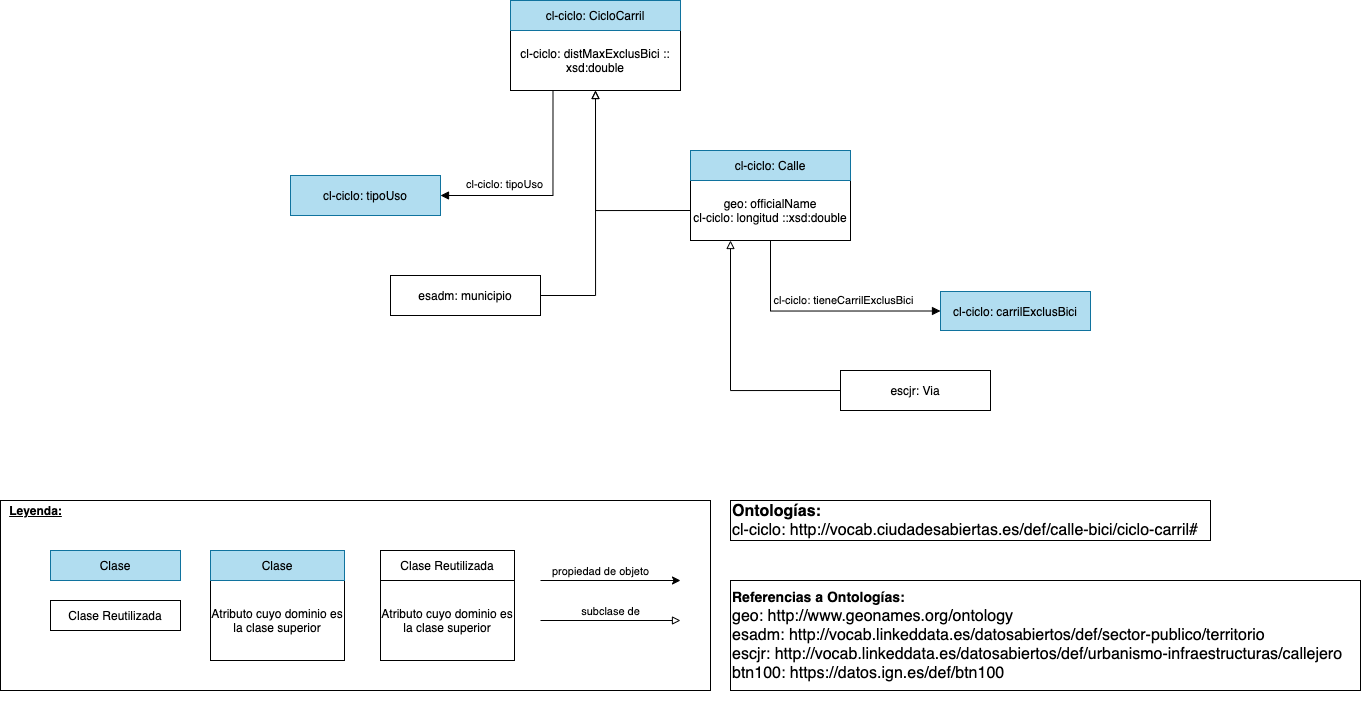
\includegraphics[angle=0, width=1\textwidth]{images/diagramaCicloCarril.png}
    \caption{Diagrama de Ontología de Ciclocarriles.}
    \label{fig:diagramaOntologCicloCarr}
\end{figure}





Para la representación de los datos de ciclocarriles para ciclistas se han definido varias clases y propiedades. Se han reutilizado elementos ya definidos en el vocabulario de Callejero de ciudadesabiertas \cite{ciudadesbiertas_callejero} y de Territorio \cite{datoabiertos_municipio}.\newline
Se han añadido elementos como el identificador de via y el municipio (que siempre será Madrid).
El identificador de vía se añadirá para cada caso a partir del nombre. Para ello se hará una reducción del nombre de la via a palabras clave, proceso detallado en la sección de Transformaciones de Vocabularios, y se cruzará con el dataset del callejero de Madrid \cite{datosmadrid_callejero}.\newline
Se ha optado por omitir la propiedad ``MinSimpTol`` debido a que no aporta valor al conjunto al tener solo 2 valores, 0 para calles sin carril bici y 0.20 para calles que si disponen de él, información que puede inferirse del campo ``MaxSimpTol`` (renombrada ``distMaxExclusBici``), con valor 0 para el primer caso y valor distinto de 0 para el segundo. Para representar esto se ha añadido la propiedad “carrilExclusBici” con valor booleano indicando si dispone de ese carril exclusivo o no.\newline
La fecha proporcionada por el ayuntamiento se ha omitido debido a que no se sabe con exactitud su significado. En caso de que fuese fecha de creación del ciclocarril se debería añadir en futuras actualizaciones del vocabulario, sin embargo al ser en todos los registros la misma cabe la posibilidad de que sea la fecha de inserción en el dataset, lo cual no aporta información relevante y podría inducir a errores.\newline
Para este caso el valor de ``tipoUso`` será siempre CICLOCARRIL.\newline
Se han transformado los valores del campo longitud a metros (expresados en kilómetros en los datos de origen) para poder reutilizarlos con más facilidad.


\newpage
En la siguiente tabla se muestran los Namespaces usados.

\begin{figure}[h]
    \centering
        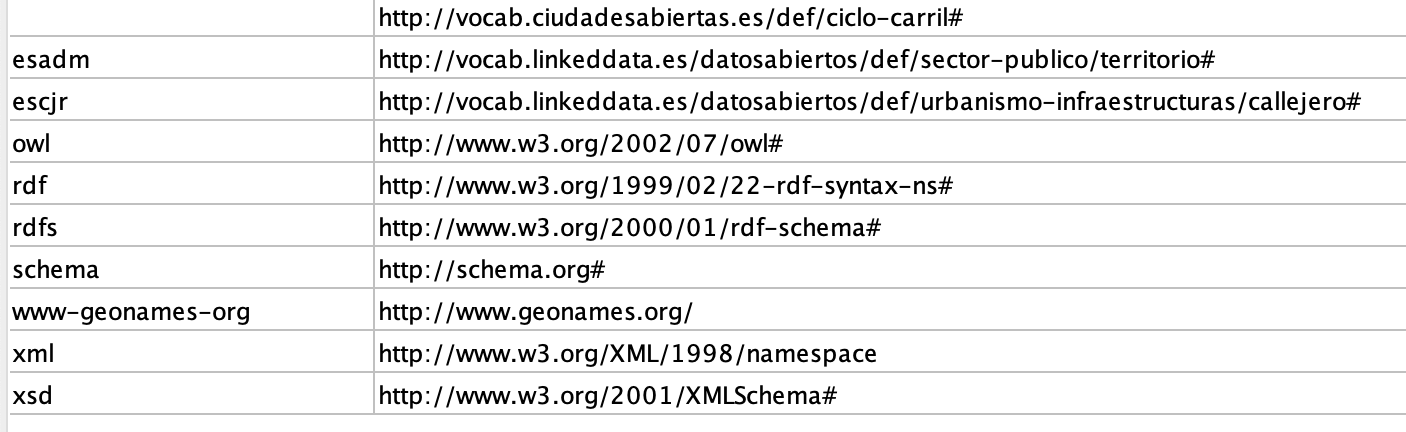
\includegraphics[angle=0, width=0.8\textwidth]{images/tablaIRIsCiclocarril.png}
    \caption{Namespaces usados para Ciclocarriles}
\end{figure}




Cabe destacar en este conjunto de datos la ausencia de la propiedad TipoVia. En este caso los nombres de las calles contenían únicamente palabras clave y privaban de la capacidad de obtener este atributo. En cambio si dispone de tipoUso, propiedad que indica si es una calle peatonal o ciclocarril.


Debido a la falta de disponibilidad de una leyenda o información proporcionada por el ayuntamiento de Madrid, para este conjunto de datos no se han podido conocer con exactitud el significado de todos sus datos y por tanto algunos como la dirección no han podido añadirse al modelo. En un futuro si se tratase información de otras fuentes o se añadiese una documentación detallada para este dataset, si se podría añadir esa propiedad.


% En este caso la fecha no aporta nada por tanto no se pone...





\clearpage
\subsection{Clases}



\begin{mybox}{CicloCarril}
\begin{flushleft}
\underline{\textbf{IRI:}}
\url{http://vocab.linkeddata.es/datosabiertos/def/urbanismo-infraestructuras/ciclo-carril#CicloCarril}
\newline

Via con uno o más carriles destinados al tránsito de ciclistas. No necesariamente exclusivos para el tránsito de bicicletas, pero si con señalización y limitaciones adaptadas para ello.
\newline

\underline{\textbf{Definida por:}}\newline
\url{http://vocab.linkeddata.es/datosabiertos/def/urbanismo-infraestructuras/ciclo-carril}
\newline

\underline{\textbf{Pertenece A:}}
	Via
\newline

\end{flushleft}
\end{mybox}

%----------------------------------------------------------------------------------------------------------------------------------------------------------------------------------------------------------------------------------------------





\begin{mybox}{Via}
\begin{flushleft}
\underline{\textbf{IRI:}}
\url{http://vocab.linkeddata.es/datosabiertos/def/urbanismo-infraestructuras/callejero#Via}
\newline

Se ha reutilizado la definición de Municipio proporcionada por vocab.linkeddata.es \cite{datoabiertos_idVia}

Vía de comunicación construida para la circulación. En su definición según el modelo de direcciones de la Administración General del Estado, Incluye calles, carreteras de todo tipo, caminos, vías de agua, pantalanes, etc. Asimismo, incluye la pseudovía., es decir todo aquello que complementa o sustituye a la vía. En nuestro caso, este término se utiliza para hacer referencia a las vías urbanas.
Representación numérica de la misma.
\newline

\underline{\textbf{Definida por:}}\newline
\url{http://vocab.linkeddata.es/datosabiertos/def/urbanismo-infraestructuras/callejero}
\newline





\end{flushleft}
\end{mybox}
%----------------------------------------------------------------------------------------------------------------------------------------------------------------------------------------------------------------------------------------------


\begin{mybox}{Municipio}
\begin{flushleft}
\underline{\textbf{IRI:}}
\url{http://vocab.linkeddata.es/datosabiertos/def/sector-publico/territorio#Municipio}
\newline

Se ha reutilizado la definición de Municipio proporcionada por vocab.linkeddata.es \cite{datoabiertos_municipio}
Un Municipio es el ente local definido en el artículo 140 de la Constitución española y la entidad básica de la organización territorial del Estado según el artículo 1 de la Ley 7/1985, de 2 de abril, Reguladora de las Bases del Régimen Local. Tiene personalidad jurídica y plena capacidad para el cumplimiento de sus fines. La delimitación territorial de Municipio está recogida del REgistro Central de Cartografía del IGN. Su nombre, que se especifica con la propiedad dct:title, es el proporcionado por el Registro de Entidades Locales del Ministerio de Política Territorial, en \url{http://www.ine.es/nomen2/index.do}
\newline


\underline{\textbf{Definida por:}}
\newline \url{http://purl.org/derecho/vocabulario}
\newline \url{http://vocab.linkeddata.es/datosabiertos/def/sector-publico/territorio}
\newline \url{http://www.ign.es/ign/resources/acercaDe/tablon/ModeloDireccionesAGE}
\newline

\underline{\textbf{Esta en rango de:}}
\newline municipio

%\underline{\textbf{Tiene Superclases:}}
%\newline CicloCarril



\end{flushleft}
\end{mybox}
%----------------------------------------------------------------------------------------------------------------------------------------------------------------------------------------------------------------------------------------------




%----------------------------------------------------------------------------------------------------------------------------------------------------------------------------------------------------------------------------------------------
%----------------------------------------------------------------------------------------------------------------------------------------------------------------------------------------------------------------------------------------------
%----------------------------------------------------------------------------------------------------------------------------------------------------------------------------------------------------------------------------------------------
%----------------------------------------------------------------------------------------------------------------------------------------------------------------------------------------------------------------------------------------------



\clearpage
\subsection{Propiedades de datos}
%----------------------------------------------------------------------------------------------------------------------------------------------------------------------------------------------------------------------------------------------
%----------------------------------------------------------------------------------------------------------------------------------------------------------------------------------------------------------------------------------------------
%----------------------------------------------------------------------------------------------------------------------------------------------------------------------------------------------------------------------------------------------
%----------------------------------------------------------------------------------------------------------------------------------------------------------------------------------------------------------------------------------------------


\begin{mybox}{longitud}
\begin{flushleft}
\underline{\textbf{IRI:}}
\url{http://vocab.linkeddata.es/datosabiertos/def/urbanismo-infraestructuras/callejero#longitud}
\newline

Longitud de la calle descrita. Esta propiedad está referida a la vía que contiene un ciclocarril (calle completa).
\newline

\underline{\textbf{Definida por:}}\newline
\url{http://vocab.linkeddata.es/datosabiertos/def/urbanismo-infraestructuras/callejero}
\newline

\underline{\textbf{Dominio:}}
	Via
\newline

\underline{\textbf{Rango:}}
		xsd:double
\newline

\end{flushleft}
\end{mybox}
%----------------------------------------------------------------------------------------------------------------------------------------------------------------------------------------------------------------------------------------------



\begin{mybox}{distMaxExclusBici}
\begin{flushleft}
\underline{\textbf{IRI:}}
\url{http://vocab.linkeddata.es/datosabiertos/def/urbanismo-infraestructuras/ciclo-carril#distMaxExclusBici}
\newline

Longitud del carril exclusivo de bicicletas dentro de la calle.
En caso de que no haya ciclocarril, el valor será 0.
\newline


\underline{\textbf{Definida por:}}\newline
\url{http://vocab.linkeddata.es/datosabiertos/def/urbanismo-infraestructuras/ciclo-carril}
\newline

\underline{\textbf{Dominio:}}
	CicloCarril
\newline

\underline{\textbf{Rango:}}
	xsd:double
\newline

\end{flushleft}
\end{mybox}
%----------------------------------------------------------------------------------------------------------------------------------------------------------------------------------------------------------------------------------------------



\begin{mybox}{officialName}
\begin{flushleft}
\underline{\textbf{IRI:}}
\url{http://www.geonames.org/ontology#officialName}
\newline

Definido en el callejero de DatosAbiertos \cite{ciudadesbiertas_callejero}.
Un nombre en el idioma oficial local.
\newline


\underline{\textbf{Definida por:}}\newline
\url{http://www.geonames.org/ontology}
\newline

\underline{\textbf{Dominio:}}
	Via
\newline

\underline{\textbf{Rango:}}
	xsd:string
\newline


\end{flushleft}
\end{mybox}
%----------------------------------------------------------------------------------------------------------------------------------------------------------------------------------------------------------------------------------------------






\begin{mybox}{carrilExclusBici}
\begin{flushleft}
\underline{\textbf{IRI:}}
\url{http://vocab.linkeddata.es/datosabiertos/def/urbanismo-infraestructuras/ciclo-carril#carril-exclus-bici}
\newline

Indicador de si las bicicletas disponen o no de un carril propio para su circulación.
\newline


\underline{\textbf{Definida por:}}\newline
\url{http://vocab.linkeddata.es/datosabiertos/def/urbanismo-infraestructuras/ciclo-carril}
\newline

\underline{\textbf{Dominio:}}
	CicloCarril
\newline

\underline{\textbf{Rango:}}
	xsd:boolean
\newline

\end{flushleft}
\end{mybox}
%----------------------------------------------------------------------------------------------------------------------------------------------------------------------------------------------------------------------------------------------







\begin{mybox}{codigoINE}
\begin{flushleft}
\underline{\textbf{IRI:}}
\url{http://vocab.linkeddata.es/datosabiertos/def/sector-publico/territorio#codigoINE}
\newline

Indicador de si las bicicletas disponen o no de un carril propio para su circulación.
\newline


\underline{\textbf{Definida por:}}\newline
\url{http://vocab.linkeddata.es/datosabiertos/def/sector-publico/territorio}
\newline

\underline{\textbf{Dominio:}}
	Municipio
\newline

\underline{\textbf{Rango:}}
	xsd:integer
\newline

\end{flushleft}
\end{mybox}
%----------------------------------------------------------------------------------------------------------------------------------------------------------------------------------------------------------------------------------------------






























\clearpage
\subsection{Propiedades de objeto}
%----------------------------------------------------------------------------------------------------------------------------------------------------------------------------------------------------------------------------------------------
%----------------------------------------------------------------------------------------------------------------------------------------------------------------------------------------------------------------------------------------------
%----------------------------------------------------------------------------------------------------------------------------------------------------------------------------------------------------------------------------------------------
%----------------------------------------------------------------------------------------------------------------------------------------------------------------------------------------------------------------------------------------------


\begin{mybox}{tieneCalle}
\begin{flushleft}
\underline{\textbf{IRI:}}
\url{http://vocab.linkeddata.es/datosabiertos/def/urbanismo-infraestructuras/ciclo-carril#tieneCalle}
\newline

Calle asociada a un CicloCarril.
\newline

\underline{\textbf{Definida por:}}
\url{http://vocab.linkeddata.es/datosabiertos/def/urbanismo-infraestructuras/ciclo-carril}
\newline

\underline{\textbf{Dominio:}}
		CicloCarril
\newline

\underline{\textbf{Rango:}}
		Calle
\newline


\end{flushleft}
\end{mybox}
%----------------------------------------------------------------------------------------------------------------------------------------------------------------------------------------------------------------------------------------------



\begin{mybox}{tipoUso}
\begin{flushleft}
\underline{\textbf{IRI:}}
\url{http://vocab.linkeddata.es/datosabiertos/def/urbanismo-infraestructuras/callejero#tipo-uso}
\newline

Identificador del tipo de uso que puede tener la calle. Se han definido 2 clases para ello:
\newline -	\url{http://vocab.ciudadesabiertas.es/kos/urbanismo-infraestructuras/calle/tipo-uso/CICLOCALLE}
\newline -	 \url{http://vocab.ciudadesabiertas.es/kos/urbanismo-infraestructuras/calle/tipo-uso/PEATONAL}
\newline


\underline{\textbf{Definida por:}}
\url{http://vocab.linkeddata.es/datosabiertos/def/urbanismo-infraestructuras/ciclo-carril}
\newline

\underline{\textbf{Dominio:}}
\newline CicloCarril

\underline{\textbf{Rango:}}
		concept


\end{flushleft}
\end{mybox}
%----------------------------------------------------------------------------------------------------------------------------------------------------------------------------------------------------------------------------------------------






\begin{mybox}{tieneIdVia}
\begin{flushleft}
\underline{\textbf{IRI:}}
\url{http://vocab.linkeddata.es/datosabiertos/def/urbanismo-infraestructuras/ciclo-carril#tieneIdVia}
\newline

Identificador de calle asociado.
\newline

\underline{\textbf{Definida por:}}
\url{http://vocab.linkeddata.es/datosabiertos/def/urbanismo-infraestructuras/ciclo-carril}
\newline

\underline{\textbf{Dominio:}}
		Calle
\newline

\underline{\textbf{Rango:}}
		Via
\newline


\end{flushleft}
\end{mybox}
%----------------------------------------------------------------------------------------------------------------------------------------------------------------------------------------------------------------------------------------------





\begin{mybox}{municipio}
\begin{flushleft}
\underline{\textbf{IRI:}}
\url{http://vocab.linkeddata.es/datosabiertos/def/sector-publico/territorio#municipio}
\newline

Municipio al que pertenece un fenómeno geográfico o una entidad administrativa.
\newline

\underline{\textbf{Definida por:}}
\url{http://vocab.linkeddata.es/datosabiertos/def/sector-publico/territorio}
\newline

\underline{\textbf{Dominio:}}
		CicloCarril
\newline

\underline{\textbf{Rango:}}
		Municipio

\end{flushleft}
\end{mybox}



%----------------------------------------------------------------------------------------------------------------------------------------------------------------------------------------------------------------------------------------------















\begin{mybox}{tieneCarrilExclusBici}
\begin{flushleft}
\underline{\textbf{IRI:}}
\url{http://vocab.linkeddata.es/datosabiertos/def/urbanismo-infraestructuras/ciclo-carril#tieneCarrilExclusBici}
\newline

Indicador de si las bicicletas disponen o no de un carril propio para su circulación.Se han definido 2 clases para ello:
\newline -	\url{http://vocab.ciudadesabiertas.es/recurso/calle-bici/ciclo-carril/carrilExlus/EXCLUSIVO-BICI}
\newline -	 \url{http://vocab.ciudadesabiertas.es/recurso/calle-bici/ciclo-carril/carrilExlus/NO-EXLUSIVO-BICI}
\newline


\underline{\textbf{Definida por:}}
\url{http://vocab.linkeddata.es/datosabiertos/def/urbanismo-infraestructuras/ciclo-carril}
\newline

\underline{\textbf{Dominio:}}
	CicloCarril
\newline

\underline{\textbf{Rango:}}
	concept
\newline

\end{flushleft}
\end{mybox}
%----------------------------------------------------------------------------------------------------------------------------------------------------------------------------------------------------------------------------------------------











%----------------------------------------------------------------------------------------------------------------------------------------------------------------------------------------------------------------------------------------------

\clearpage
\section{Vocabulario de Calles Tranquilas}

Para el vocabulario asociado con las calles tranquilas para ciclistas en el ayuntamiento de Madrid se ha elegido la fuente de Datos.Madrid \cite{datosMadrid_callesTranquilas}.
Proporcionada por el ayuntamiento de Madrid, se muestran las calles más apropiadas para el tránsito de ciclistas. No se dan especificaciones de los criterios utlizados que han llevado a estas calles a formar parte de la lista. Sin embargo, si se puede observar en algnas de ellas ciertos patrones, como que no forman parte de las vias principales de la capital y que son poco transitadas. La misma web ofrece un archivo KML y permite que se puedan mostrar sobre un mapa en Open Street Map \cite{openStreetMapCallesTranquilas}, lo cual proporciona una idea general de su disposición y posibles criterios utilizados.
\newline
\newline
La organización del conjunto de datos se hará siguiendo el diagrama \ref{fig:diagramaOntologCallTranq}.

\begin{figure}[h]
	\centering
		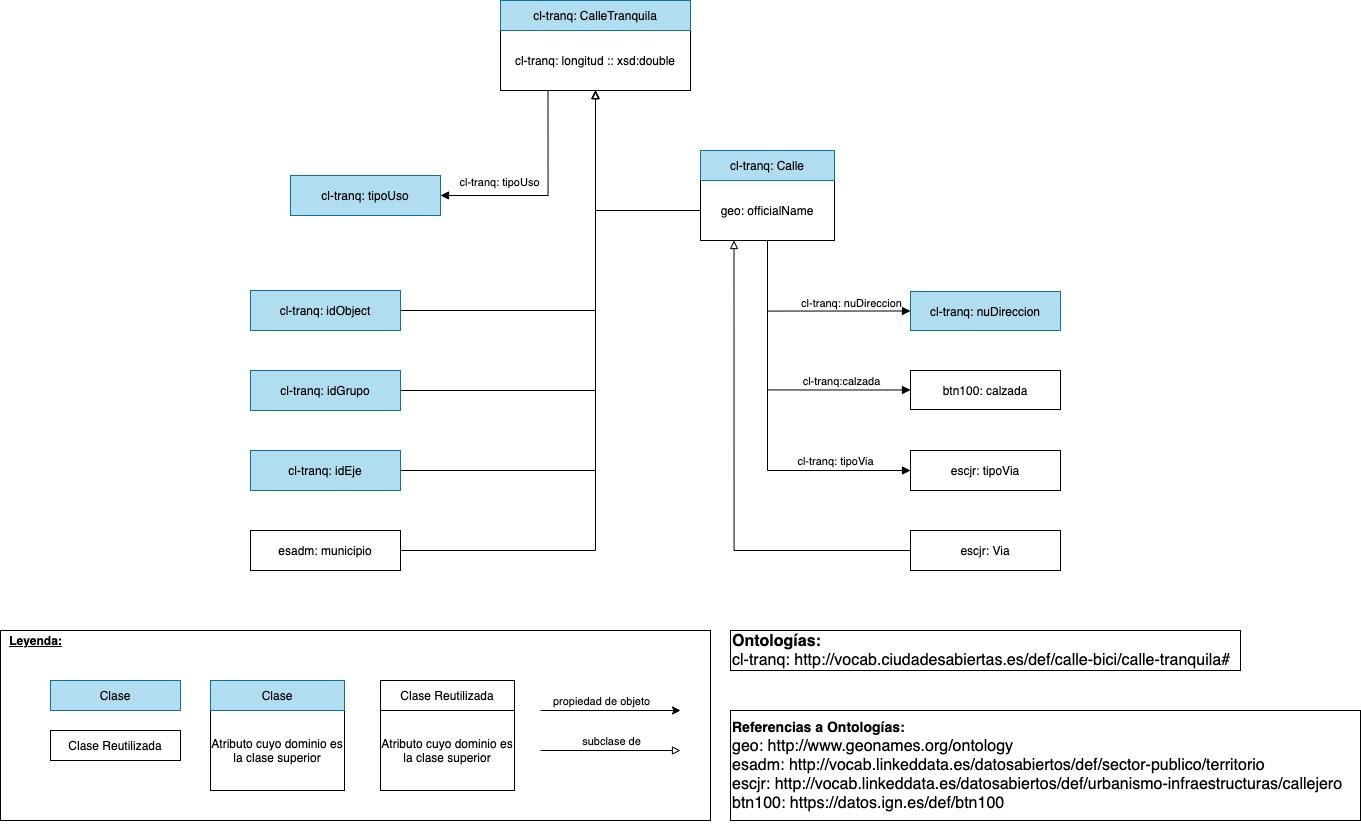
\includegraphics[angle=0, width=0.8\textwidth]{images/diagramaCallesTranqui.png}  
	\caption{Diagrama de Ontología de Calles Tranquilas en Madrid.}
	\label{fig:diagramaOntologCallTranq}
\end{figure}


Para la representación de los datos de calles tranquilas para ciclistas se han definido varias clases y propiedades. Se han tomado como ejemplo el vocabulario definido en ciudades abiertas de Callejero \cite{ciudadesbiertas_callejero} y el definido en datos.ign sobre calzadas \cite{datosIgnCalzada}.
\newline
Se han realizados ciertas modificaciones con respecto al dataset original para que puedan utilizarse sus datos más eficazmente.
Se ha optado por la separación del tipo de via del nombre, conservandola en éste y creando una nueva propiedad que permita saber su clase. Algunos ejemplos serían Calle, Avenida, Plaza...
Se ha añadido el identificador de la via, obtenido a partir del nombre y cruzado con el dataset del callejero de madrid \cite{datosmadrid_callejero}. El identificador permitirá hacer búsquedas mucho más rápidas sobre los datos en caso de querer hacerla filtrando por la calle, que es el caso de la aplicación final que se desea realizar para este proyecto.
En este caso el municipio será siempre madrid, pero en caso de que se quisiera reulizar en otros proyectos a mayor escala sería necesario conocer la zona geográfica donde se encuentra, por tanto también se ha añadido, aunque con el valor fijo de Madrid, que corresponde al código 28079, proporcionado por el Instituto Nacional de Estadistica\cite{datosIgnMunicipios}.

Estas transformaciones se detallarán más adelante en la seccion: Transformaciones en los vocabularios.

Se ha optado por omitir la propiedad ID$\_$TIPO, ya que representa lo mismo que TX$\_$CAPA (el uso que tiene la via) y se ha optado por la segunda por ser representado con texto, más visual y representativo a la hora de su utilización.

El tipo de uso se ha definido en \url{http://vocab.ciudadesabiertas.es/def/calle-bici#tipoUso} debido a que es común para todas las calle-bici (tanto calles tranquilas como ciclocarriles), por lo tanto se ha optado porque los valores sean definidos en una categoria que englobe a las dos.
La dirección se ha definido también en esta categoría común ya que podría ser añadida a ciclocarriles por el ayuntamiento o ser común con otros dataset de una categoría similar( \url{http://vocab.ciudadesabiertas.es/def/calle-bici#nuDireccion} ).

En la siguiente tabla se muestran los Namespaces usados.

\begin{figure}[h]
	\centering
		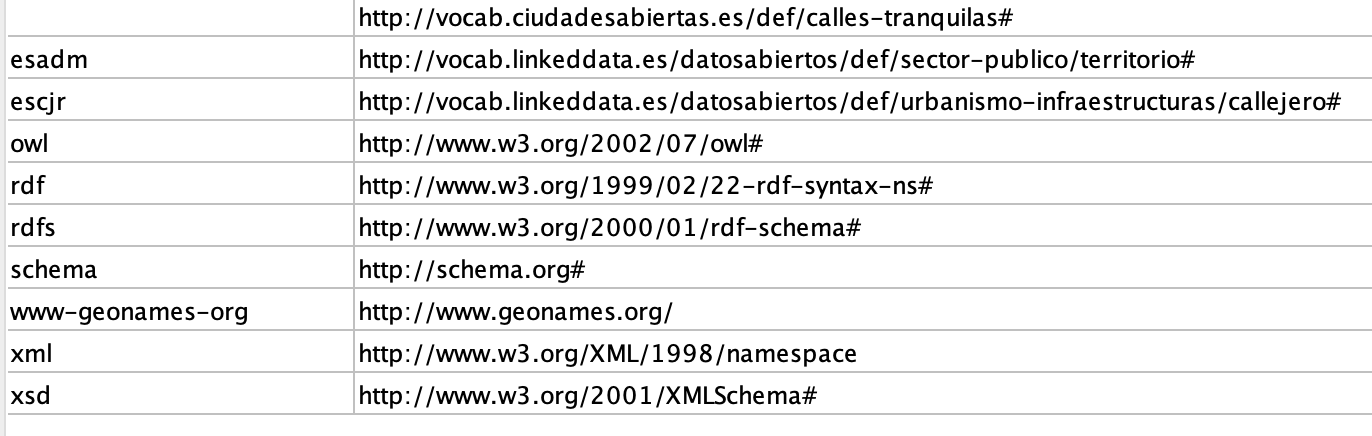
\includegraphics[angle=0, width=0.8\textwidth]{images/tablaIRIsCallesTranquilas.png}  
	\caption{Namespaces usados para Calles Tranquilas}
\end{figure}


Debido a la falta de disponibilidad de una leyenda o información proporcionada por el ayuntameinto de Madrid, para este conjunto de datos no se han podido conocer con exactitud el significado de sus datos. Se ha obtenido de forma aproximada esa información pero podria no ser correcta.



%\clearpage
%\subsection{Clases}



\begin{mybox}{CalleTranquila}
\begin{flushleft}
\underline{\textbf{IRI:}}
\url{http://vocab.ciudadesabiertas.es/def/calle-bici/calle-tranquila#CalleTranquila}
\newline

Calle apropiada para el tránsito de ciclistas siguiendo los cirterios del ayuntamiento de Madrid.
\newline

\underline{\textbf{Definida por:}}
\url{http://vocab.ciudadesabiertas.es/def/calle-bici/calle-tranquila}
\newline

\underline{\textbf{Tiene subclase:}}
\newline idObject,\hspace{2em}  idGrupo,\hspace{2em} idEje,	\hspace{2em} tipoUso,
\newline municipio,\hspace{2em} Calle

\underline{\textbf{Tiene Superclase:}}
\newline longitud

\end{flushleft}
\end{mybox}

%----------------------------------------------------------------------------------------------------------------------------------------------------------------------------------------------------------------------------------------------






\begin{mybox}{Calle}
\begin{flushleft}
\underline{\textbf{IRI:}}
\url{http://vocab.ciudadesabiertas.es/def/calle-bici/calle-tranquila#Calle}
\newline

Representación de una via de una ciudad.
\newline

\underline{\textbf{Definida por:}}
\url{http://vocab.ciudadesabiertas.es/def/calle-bici/calle-tranquila}
\newline

\underline{\textbf{Tiene subclase:}}
\newline longitud,\hspace{2em}  nuDireccion,
\newline calzada,\hspace{2em} tipoVia

\underline{\textbf{Tiene Superclases:}}
\newline CalleTranquila
\newline nombre oficial

\end{flushleft}
\end{mybox}

%----------------------------------------------------------------------------------------------------------------------------------------------------------------------------------------------------------------------------------------------






\begin{mybox}{Via}
\begin{flushleft}
\underline{\textbf{IRI:}}
\url{http://vocab.linkeddata.es/datosabiertos/def/urbanismo-infraestructuras/callejero#Via}
\newline

Se ha reutilizado la definición de Municipio proporcionada por vocab.linkeddata.es \cite{datoabiertos_idVia}

Vía de comunicación construida para la circulación. En su definición según el modelo de direcciones de la Administración General del Estado, Incluye calles, carreteras de todo tipo, caminos, vías de agua, pantalanes, etc. Asimismo, incluye la pseudovía., es decir todo aquello que complementa o sustituye a la vía. En nuestro caso, este término se utiliza para hacer referencia a las vías urbanas.
Representación numérica de la misma.
\newline

\underline{\textbf{Definida por:}}
\url{http://vocab.linkeddata.es/datosabiertos/def/urbanismo-infraestructuras/callejero}
\newline

\underline{\textbf{Tiene Superclases:}}
\newline Calle





\end{flushleft}
\end{mybox}
%----------------------------------------------------------------------------------------------------------------------------------------------------------------------------------------------------------------------------------------------




\begin{mybox}{Municipio}
\begin{flushleft}
\underline{\textbf{IRI:}}
\url{http://vocab.linkeddata.es/datosabiertos/def/sector-publico/territorio#Municipio}
\newline

Se ha reutilizado la definición de Municipio proporcionada por vocab.linkeddata.es \cite{datoabiertos_municipio}
Un Municipio es el ente local definido en el artículo 140 de la Constitución española y la entidad básica de la organización territorial del Estado según el artículo 1 de la Ley 7/1985, de 2 de abril, Reguladora de las Bases del Régimen Local. Tiene personalidad jurídica y plena capacidad para el cumplimiento de sus fines. La delimitación territorial de Municipio está recogida del REgistro Central de Cartografía del IGN. Su nombre, que se especifica con la propiedad dct:title, es el proporcionado por el Registro de Entidades Locales del Ministerio de Política Territorial, en \url{http://www.ine.es/nomen2/index.do}
\newline


\underline{\textbf{Definida por:}}
\url{http://purl.org/derecho/vocabulario}
\url{http://vocab.linkeddata.es/datosabiertos/def/sector-publico/territorio}
\url{http://www.ign.es/ign/resources/acercaDe/tablon/ModeloDireccionesAGE}
\newline

\underline{\textbf{Tiene Superclases:}}
\newline CalleTranquila



\end{flushleft}
\end{mybox}
%----------------------------------------------------------------------------------------------------------------------------------------------------------------------------------------------------------------------------------------------





\begin{mybox}{idObject}
\begin{flushleft}
\underline{\textbf{IRI:}}
\url{http://vocab.ciudadesabiertas.es/def/calle-bici/calle-tranquila#idObject}
\newline

Identificador propio del ayuntamiento.
%\newline{A la espera de conocer su significado}
\newline


\underline{\textbf{Definida por:}}
\url{http://vocab.ciudadesabiertas.es/def/calle-bici/calle-tranquila}
\newline

\underline{\textbf{Tiene Superclases:}}
\newline CalleTranquila

\end{flushleft}
\end{mybox}
%----------------------------------------------------------------------------------------------------------------------------------------------------------------------------------------------------------------------------------------------




\begin{mybox}{idGrupo}
\begin{flushleft}
\underline{\textbf{IRI:}}
\url{http://vocab.ciudadesabiertas.es/def/calle-bici/calle-tranquila#idGrupo}
\newline

Identificador propio del ayuntamiento. 
%\newline{A la espera de conocer su significado}
\newline

\underline{\textbf{Definida por:}}
\url{http://vocab.ciudadesabiertas.es/def/calle-bici/calle-tranquila}
\newline

\underline{\textbf{Tiene Superclases:}}
\newline CalleTranquila

\end{flushleft}
\end{mybox}
%----------------------------------------------------------------------------------------------------------------------------------------------------------------------------------------------------------------------------------------------




\begin{mybox}{idEje}
\begin{flushleft}
\underline{\textbf{IRI:}}
\url{http://vocab.ciudadesabiertas.es/def/calle-bici/calle-tranquila#idEje}
\newline

Identificador propio del ayuntamiento. 
%\newline{A la espera de conocer su significado}
\newline


\underline{\textbf{Definida por:}}
\url{http://vocab.ciudadesabiertas.es/def/calle-bici/calle-tranquila}
\newline

\underline{\textbf{Tiene Superclases:}}
\newline CalleTranquila

\end{flushleft}
\end{mybox}
%----------------------------------------------------------------------------------------------------------------------------------------------------------------------------------------------------------------------------------------------







%----------------------------------------------------------------------------------------------------------------------------------------------------------------------------------------------------------------------------------------------
%----------------------------------------------------------------------------------------------------------------------------------------------------------------------------------------------------------------------------------------------
%----------------------------------------------------------------------------------------------------------------------------------------------------------------------------------------------------------------------------------------------
%----------------------------------------------------------------------------------------------------------------------------------------------------------------------------------------------------------------------------------------------



%\clearpage
%\subsection{Propiedades de datos}
%----------------------------------------------------------------------------------------------------------------------------------------------------------------------------------------------------------------------------------------------
%----------------------------------------------------------------------------------------------------------------------------------------------------------------------------------------------------------------------------------------------
%----------------------------------------------------------------------------------------------------------------------------------------------------------------------------------------------------------------------------------------------
%----------------------------------------------------------------------------------------------------------------------------------------------------------------------------------------------------------------------------------------------




\begin{mybox}{nombre oficial}
\begin{flushleft}
\underline{\textbf{IRI:}}
\url{http://www.geonames.org/ontology#officialName}
\newline

Definido en el callejero de DatosAbiertos \cite{ciudadesbiertas_callejero}.
Un nombre en el idioma oficial local.
\newline


\underline{\textbf{Definida por:}}
\url{http://www.geonames.org/ontology}
\newline

\underline{\textbf{Dominio:}}
	Calle
\newline


\end{flushleft}
\end{mybox}
%----------------------------------------------------------------------------------------------------------------------------------------------------------------------------------------------------------------------------------------------





\begin{mybox}{longitud}
\begin{flushleft}
\underline{\textbf{IRI:}}
\url{http://vocab.ciudadesabiertas.es/def/calle-bici/calle-tranquila#longitud}
\newline

Longitud de la calle o tramo de la calle descrito. Su medida es Shape$\_$leng.
Es propiedad de CalleTranquila y no de calle porque cabe la posibilidad de que no coincidan ambas medidas debido a tramos de vias más inseguros. A falta de documentación sobre el dataset se ha supuesto esta hipótesis.
\newline

\underline{\textbf{Definida por:}}
\url{http://vocab.ciudadesabiertas.es/def/calle-bici/calle-tranquila}
\newline

\underline{\textbf{Dominio:}}
		CalleTranquila
\newline

\underline{\textbf{Rango:}}
		double

\end{flushleft}
\end{mybox}
%----------------------------------------------------------------------------------------------------------------------------------------------------------------------------------------------------------------------------------------------














%\clearpage
%\subsection{Propiedades de objeto}
%----------------------------------------------------------------------------------------------------------------------------------------------------------------------------------------------------------------------------------------------
%----------------------------------------------------------------------------------------------------------------------------------------------------------------------------------------------------------------------------------------------
%----------------------------------------------------------------------------------------------------------------------------------------------------------------------------------------------------------------------------------------------
%----------------------------------------------------------------------------------------------------------------------------------------------------------------------------------------------------------------------------------------------



\begin{mybox}{tieneCalle}
\begin{flushleft}
\underline{\textbf{IRI:}}
\url{http://vocab.ciudadesabiertas.es/def/calle-bici/calle-tranquila#tieneCalle}
\newline

Calle asociada a una Calle Tranquila.
\newline

\underline{\textbf{Definida por:}}
\url{http://vocab.ciudadesabiertas.es/def/calle-bici/calle-tranquila}
\newline

\underline{\textbf{Dominio:}}
		CalleTranquila
\newline

\underline{\textbf{Rango:}}
		Calle
\newline


\end{flushleft}
\end{mybox}
%----------------------------------------------------------------------------------------------------------------------------------------------------------------------------------------------------------------------------------------------



\begin{mybox}{tipoUso}
\begin{flushleft}
\underline{\textbf{IRI:}}
\url{http://vocab.ciudadesabiertas.es/def/calle-bici/calle-tranquila#tipoUso}
\newline

Identificador del tipo de uso que puede tener la calle. Se han definido 2 clases para ello:
\newline -	\url{http://vocab.ciudadesabiertas.es/recurso/calle-bici/tipoUso/CICLOCALLE}
\newline -	 \url{http://vocab.ciudadesabiertas.es/recurso/calle-bici/tipoUso/PEATONAL}
\newline


%\underline{\textbf{Definida por:}}
%\url{http://vocab.ciudadesabiertas.es/def/calle-bici}
%\newline

\underline{\textbf{Dominio:}}
\newline CalleTranquila

\underline{\textbf{Rango:}}
		concept


\end{flushleft}
\end{mybox}
%----------------------------------------------------------------------------------------------------------------------------------------------------------------------------------------------------------------------------------------------



\begin{mybox}{tieneIdEje}
\begin{flushleft}
\underline{\textbf{IRI:}}
\url{http://vocab.ciudadesabiertas.es/def/calle-bici/calle-tranquila#tieneIdEje}
\newline

Identificador de Eje asociado a una calle.
\newline

\underline{\textbf{Definida por:}}
\url{http://vocab.ciudadesabiertas.es/def/calle-bici/calle-tranquila}
\newline

\underline{\textbf{Dominio:}}
		CalleTranquila
\newline

\underline{\textbf{Rango:}}
		idEje

\end{flushleft}
\end{mybox}
%----------------------------------------------------------------------------------------------------------------------------------------------------------------------------------------------------------------------------------------------





\begin{mybox}{tieneIdGrupo}
\begin{flushleft}
\underline{\textbf{IRI:}}
\url{http://vocab.ciudadesabiertas.es/def/calle-bici/calle-tranquila#tieneIdGrupo}
\newline

Identificador de Grupo asociado a una calle.
\newline

\underline{\textbf{Definida por:}}
\url{http://vocab.ciudadesabiertas.es/def/calle-bici/calle-tranquila}
\newline

\underline{\textbf{Dominio:}}
		CalleTranquila
\newline

\underline{\textbf{Rango:}}
		idGrupo

\end{flushleft}
\end{mybox}
%----------------------------------------------------------------------------------------------------------------------------------------------------------------------------------------------------------------------------------------------




\begin{mybox}{tieneIdObject}
\begin{flushleft}
\underline{\textbf{IRI:}}
\url{http://vocab.ciudadesabiertas.es/def/calle-bici/calle-tranquila#tieneIdObject}
\newline

Identificador de Objeto asociado a una calle.
\newline

\underline{\textbf{Definida por:}}
\url{http://vocab.ciudadesabiertas.es/def/calle-bici/calle-tranquila}
\newline

\underline{\textbf{Dominio:}}
		CalleTranquila
\newline

\underline{\textbf{Rango:}}
		idObject

\end{flushleft}
\end{mybox}
%----------------------------------------------------------------------------------------------------------------------------------------------------------------------------------------------------------------------------------------------






\begin{mybox}{tieneIdVia}
\begin{flushleft}
\underline{\textbf{IRI:}}
\url{http://vocab.ciudadesabiertas.es/def/calle-bici/calle-tranquila#tieneIdVia}
\newline

Identificador de calle asociado.
\newline

\underline{\textbf{Definida por:}}
\url{http://vocab.ciudadesabiertas.es/def/calle-bici/calle-tranquila}
\newline

\underline{\textbf{Dominio:}}
		Calle
\newline

\underline{\textbf{Rango:}}
		Via
\newline


\end{flushleft}
\end{mybox}
%----------------------------------------------------------------------------------------------------------------------------------------------------------------------------------------------------------------------------------------------





\begin{mybox}{tieneMunicipio}
\begin{flushleft}
\underline{\textbf{IRI:}}
\url{http://vocab.ciudadesabiertas.es/def/calle-bici/calle-tranquila#tieneMunicipio}
\newline

Municipio que contiene una calle.
\newline

\underline{\textbf{Definida por:}}
\url{http://vocab.ciudadesabiertas.es/def/calle-bici/calle-tranquila}
\newline

\underline{\textbf{Dominio:}}
		CalleTranquila
\newline

\underline{\textbf{Rango:}}
		municipio

\end{flushleft}
\end{mybox}



%----------------------------------------------------------------------------------------------------------------------------------------------------------------------------------------------------------------------------------------------





\begin{mybox}{nuDireccion}
\begin{flushleft}
\underline{\textbf{IRI:}}
\url{http://vocab.ciudadesabiertas.es/def/calle-bici#nuDireccion}
\newline

Dirección y sentido de la calle o tramo de la calle a la que se refiere.
Puede tomar los siguientes valores:
\newline \url{http://vocab.ciudadesabiertas.es/recurso/calle-bici#SOL} - Dirección y sentido a Sol
\newline \url{http://vocab.ciudadesabiertas.es/recurso/calle-bici#paraleloSOL} - Dirección paralela a Sol
\newline \url{http://vocab.ciudadesabiertas.es/recurso/calle-bici#contrarioSOL} - Dirección a sol y sentido opuesto.
\newline

Esta definición esta basada en datos aproximados proporcionados por mapas y otros elementos que han podido verse en los ejemplos del dataset. Pueden ser erróneos o no reflejar con exactitud la realidad del dato ya que no existe una leyenda que poder consultar.
\newline

%\newline http://vocab.ciudadesabiertas.es/recurso/calle-bici#1: Dirección y sentido a Sol.
%\newline http://vocab.ciudadesabiertas.es/recurso/calle-bici#0: Dirección paralela a cualquiera que apunte a Sol.
%\newline http://vocab.ciudadesabiertas.es/recurso/calle-bici#-1: Dirección a Sol, sentido opuesto.
%\newline { A la espera de conocer su significado oficial, basado en datos aproximados }


\underline{\textbf{Definida por:}}
\url{http://vocab.ciudadesabiertas.es/def/calle-bici}
\newline

\underline{\textbf{Dominio:}}
		Calle
\newline

\underline{\textbf{Rango}}
\newline concept

\end{flushleft}
\end{mybox}
%----------------------------------------------------------------------------------------------------------------------------------------------------------------------------------------------------------------------------------------------






\begin{mybox}{calzada}
\begin{flushleft}
\underline{\textbf{IRI:}}
\url{https://datos.ign.es/def/btn100#calzada}
\newline

Doble sentido o sentido único de una calle.
Puede tomar los siguientes valores definidos en datos.ign.es \cite{datosIgn_calzada}:
%\newline 1: Calle de doble sentido.
%\newline 0: Calle de sentido único.
%\newline { A la espera de conocer su significado oficial, basado en datos aproximados }
\newline \url{https://datos.ign.es/kos/transportes/calzada/convencional}
\newline \url{https://datos.ign.es/kos/transportes/calzada/doble}
\newline \url{https://datos.ign.es/kos/transportes/calzada/sentido-unico}
\newline

\underline{\textbf{Definida por:}}
\url{https://datos.ign.es/kos/transportes/calzada/}
\newline

\underline{\textbf{Dominio:}}
		Calle
\newline

\underline{\textbf{Rango:}}
\newline concept

\end{flushleft}
\end{mybox}
%----------------------------------------------------------------------------------------------------------------------------------------------------------------------------------------------------------------------------------------------














\begin{mybox}{tipoVia}
\begin{flushleft}
\underline{\textbf{IRI:}}
\url{http://vocab.linkeddata.es/datosabiertos/def/urbanismo-infraestructuras/callejero#tipoVia}
\newline

Se ha reutilizado la definición de tipoVia proporcionada por vocab.linkeddata.es \cite{datoabiertos_tipoVia}.
Tipo de vía, que será representado mediante la clasificación en SKOS de URI \url{http://vocab.linkeddata.es/datosabiertos/kos/urbanismo-infraestructuras/tipo-via}. Por ejemplo, estas serán las URIs correspondientes a calles y plazas \url{http://vocab.linkeddata.es/datosabiertos/kos/urbanismo-infraestructuras/tipo-via/CL} \url{http://vocab.linkeddata.es/datosabiertos/kos/urbanismo-infraestructuras/tipo-via/PL}
\newline

\underline{\textbf{Definida por:}}
\url{http://vocab.linkeddata.es/datosabiertos/def/urbanismo-infraestructuras/callejero}
\newline

\underline{\textbf{Dominio:}}
		Calle
\newline

\underline{\textbf{Rango:}}
		concept

\end{flushleft}
\end{mybox}
%----------------------------------------------------------------------------------------------------------------------------------------------------------------------------------------------------------------------------------------------


























%----------------------------------------------------------------------------------------------------------------------------------------------------------------------------------------------------------------------------------------------


\clearpage
\section{Vocabulario de Callejero (Propuesta)}

La objetivo final de este proyecto es construir una aplicación que permita cruzar datos relativos a bicicletas en Madrid para así obtener la seguridad de una ruta. Muchos de ellos no pueden considerarse propios de las bicicletas sino que forman parte de las vías por las que éstas van a circular. La necesidad de estos datos y las posibles utilidades que podrían tener para muchos otras otras aplicaciones y tratamientos han llevado a realizar una propuesta de modificación al propio vocabulario de callejero ya creado.\newline
Aun siendo cambios menores que no afectan a la estructura ni a la base del mismo, si es necesario realizar esta ampliación para que pueda abarcar más información y pueda tener muchas más aplicaciones.\newline
Para ello se ha abierto una petición en Github para este repositorio y una vez aceptada formaría parte del modelo.
\newline
\newline
En el diagrama \ref{fig:diagramaOntologCicloCarr} se muestran las modificaciones propuestas en rojo. También como parte del proyecto se ha modificado el gráfico para que siga el formato de las nuevas ontologías que se estaban creando en ciudadesabiertas \cite{ciudadesabiertas_catalogoVocabs}

\begin{figure}[h]
	\centering
		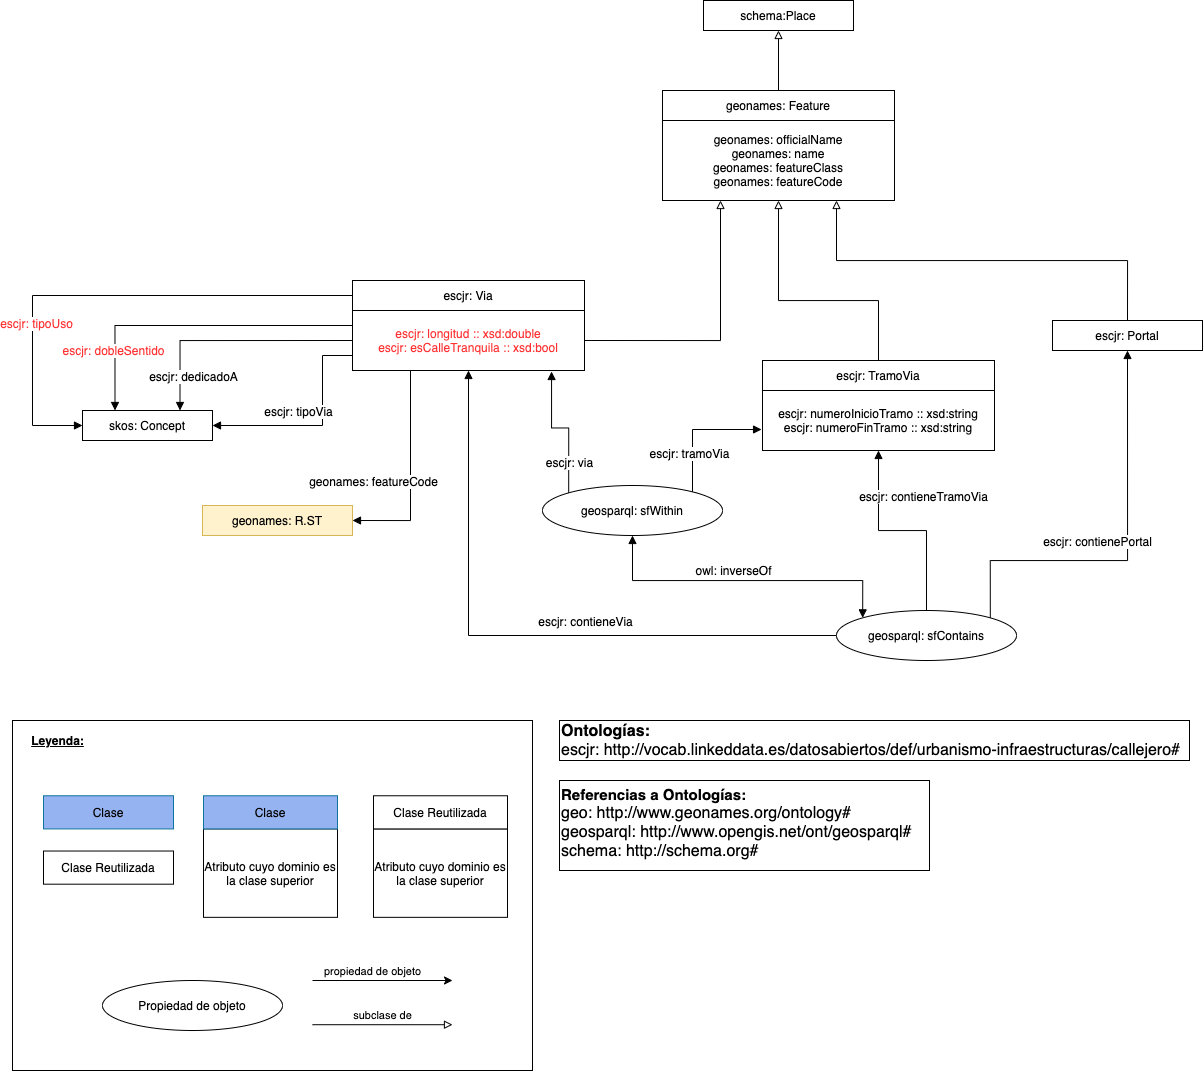
\includegraphics[angle=0, width=1\textwidth]{images/diagramaCallejero.png}  
	\caption{Diagrama de Ontología de Callejero}
	\label{fig:diagramaOntologCicloCarr}
\end{figure}


Se han añadadido las propiedades de objeto tipoUso y dobeSentido. La primera de ellas ha sido utilizada en los datasets de CicloCarriles y de CallesTranquilas y se refiere al uso dado (CicloCarril o Peatonal). La segunda únicamente en CallesTranquilas y como su nombre indica, representa el sentido único o doble de una calle.\newline
Se han añadido además dos propiedades de datos para la clase Via: longitud y esCalleTranquila. La primera se representa con un valor numérico decimal y formaba parte del dataset de Ciclocarriles y de CallesTranquilas. La segunda representa con un valor booleano si es o no una calle tranquila para ciclistas siguiendo el criterio del ayuntamiento.\newline
En las siguientes secciones se detallarán estas propiedades incluidas en la propuesta de modificación.

Este vocabulario ha sido propuesto para ser incluido en el repositorio opencitydata en los siguientes ISSUEs 
\url{https://github.com/opencitydata/urbanismo-infraestructuras-callejero/issues/18}
\url{https://github.com/opencitydata/urbanismo-infraestructuras-callejero/issues/19}
\url{https://github.com/opencitydata/urbanismo-infraestructuras-callejero/issues/20}
\url{https://github.com/opencitydata/urbanismo-infraestructuras-callejero/issues/21}
\url{https://github.com/opencitydata/urbanismo-infraestructuras-callejero/issues/22}



\clearpage
\subsection{Propiedades de datos}
%----------------------------------------------------------------------------------------------------------------------------------------------------------------------------------------------------------------------------------------------
%----------------------------------------------------------------------------------------------------------------------------------------------------------------------------------------------------------------------------------------------
%----------------------------------------------------------------------------------------------------------------------------------------------------------------------------------------------------------------------------------------------
%----------------------------------------------------------------------------------------------------------------------------------------------------------------------------------------------------------------------------------------------




\begin{mybox}{esCalleTranquila}
\begin{flushleft}
\underline{\textbf{IRI:}}
\url{http://vocab.linkeddata.es/datosabiertos/def/urbanismo-infraestructuras/callejero#esCalleTranquila}
\newline

Propiedad que indica si una vía es calle tranquila o no para bicicletas. Vías con poco tráfico, mucha visibilidad o con mucho porcentaje de accidentes pueden ser algunos de los criterios seguidos para esta valoración.
\newline


\underline{\textbf{Definida por:}}\newline
\url{http://vocab.linkeddata.es/datosabiertos/def/urbanismo-infraestructuras/callejero}
\newline

\underline{\textbf{Dominio:}}
	Via
\newline

\underline{\textbf{Rango:}}
		xsd:boolean

\end{flushleft}
\end{mybox}
%----------------------------------------------------------------------------------------------------------------------------------------------------------------------------------------------------------------------------------------------





\begin{mybox}{longitud}
\begin{flushleft}
\underline{\textbf{IRI:}}
\url{http://vocab.linkeddata.es/datosabiertos/def/urbanismo-infraestructuras/callejero#longitud}
\newline

Longitud de la calle o tramo de la calle descrito. Su unidad de medida es el metro aunque en muchos casos puede venir representado como Shape$\_$leng.
\newline

\underline{\textbf{Definida por:}}\newline
\url{http://vocab.linkeddata.es/datosabiertos/def/urbanismo-infraestructuras/callejero}
\newline

\underline{\textbf{Dominio:}}
		Via
\newline

\underline{\textbf{Rango:}}
		xsd:double

\end{flushleft}
\end{mybox}
%----------------------------------------------------------------------------------------------------------------------------------------------------------------------------------------------------------------------------------------------







\begin{mybox}{dobleSentido}
\begin{flushleft}
\underline{\textbf{IRI:}}
\url{http://vocab.linkeddata.es/datosabiertos/def/urbanismo-infraestructuras/callejero#dobleSentido}
\newline

Propiedad que determina si una vía es de sentido único o doble.
%Puede tomar los siguientes valores definidos en datos.ign.es \cite{datosIgn_calzada}:
%\newline 1: Calle de doble sentido.
%\newline 0: Calle de sentido único.
%\newline { A la espera de conocer su significado oficial, basado en datos aproximados }
%\newline \url{http://vocab.ciudadesabiertas.es/kos/urbanismo-infraestructuras/calle/doble-sentido/SENTIDO-UNICO}
%\newline \url{http://vocab.ciudadesabiertas.es/kos/urbanismo-infraestructuras/calle/doble-sentido/DOBLE-SENTIDO}
\newline

\underline{\textbf{Definida por:}}\newline
\url{http://vocab.linkeddata.es/datosabiertos/def/urbanismo-infraestructuras/callejero}
\newline

\underline{\textbf{Dominio:}}
		Via
\newline

\underline{\textbf{Rango:}}
 xsd: boolean
 \newline

\end{flushleft}
\end{mybox}
%----------------------------------------------------------------------------------------------------------------------------------------------------------------------------------------------------------------------------------------------













\clearpage
\subsection{Propiedades de objeto}
%----------------------------------------------------------------------------------------------------------------------------------------------------------------------------------------------------------------------------------------------
%----------------------------------------------------------------------------------------------------------------------------------------------------------------------------------------------------------------------------------------------
%----------------------------------------------------------------------------------------------------------------------------------------------------------------------------------------------------------------------------------------------
%----------------------------------------------------------------------------------------------------------------------------------------------------------------------------------------------------------------------------------------------




\begin{mybox}{tipoUso}
\begin{flushleft}
\underline{\textbf{IRI:}}
\url{http://vocab.linkeddata.es/datosabiertos/def/urbanismo-infraestructuras/callejero#tipoUso}
\newline

Identificador del tipo de uso que puede tener la calle. Se han definido 2 clases para ello:
\newline -	\url{http://vocab.ciudadesabiertas.es/kos/urbanismo-infraestructuras/calle/tipo-uso/CICLOCALLE}
\newline -	 \url{http://vocab.ciudadesabiertas.es/kos/urbanismo-infraestructuras/calle/tipo-uso/PEATONAL}
\newline


\underline{\textbf{Definida por:}}
\url{http://vocab.linkeddata.es/datosabiertos/def/urbanismo-infraestructuras/callejero}
\newline

\underline{\textbf{Dominio:}} Via
\newline

\underline{\textbf{Rango:}}
	concept
\newline


\end{flushleft}
\end{mybox}
%----------------------------------------------------------------------------------------------------------------------------------------------------------------------------------------------------------------------------------------------





\begin{mybox}{dobleSentido}
\begin{flushleft}
\underline{\textbf{IRI:}}
\url{http://vocab.linkeddata.es/datosabiertos/def/urbanismo-infraestructuras/callejero#dobleSentido}
\newline

Doble sentido o sentido único de una calle.
Puede tomar los siguientes valores definidos en datos.ign.es \cite{datosIgn_calzada}:
%\newline 1: Calle de doble sentido.
%\newline 0: Calle de sentido único.
%\newline { A la espera de conocer su significado oficial, basado en datos aproximados }
\newline \url{http://vocab.ciudadesabiertas.es/kos/urbanismo-infraestructuras/calle/doble-sentido/SENTIDO-UNICO}
\newline \url{http://vocab.ciudadesabiertas.es/kos/urbanismo-infraestructuras/calle/doble-sentido/DOBLE-SENTIDO}
\newline

\underline{\textbf{Definida por:}}\newline
\url{http://vocab.linkeddata.es/datosabiertos/def/urbanismo-infraestructuras/callejero}
\newline

\underline{\textbf{Dominio:}}
		Via
\newline

\underline{\textbf{Rango:}}
 concept
 \newline

\end{flushleft}
\end{mybox}
%----------------------------------------------------------------------------------------------------------------------------------------------------------------------------------------------------------------------------------------------















%----------------------------------------------------------------------------------------------------------------------------------------------------------------------------------------------------------------------------------------------






\clearpage
\chapter{Transformaciones en los Datasets}

Partiendo de los datos proporcionados por el ayuntamiento de Madrid y con el fin de plasmar las estructuras antes definidas, se han realizados ciertos cambios con respecto al dataset original. Campos añadidos, modificaciones o transformaciones en los ya existentes son algunos de los motivos para realizarlos.

Cabe destacar que antes de hacer cualquier modificación o tratamiento se deben transformar a codificación ISO-8859-1. En los datasets utilizados para este proyecto, obtenidos de la web de datos abiertos del ayuntamiento de Madrid \cite{datosabiertos_ayuntmadrid}, se han observado muchos problemas en torno a su codificación.

Para este proyecto, como ya se ha mencionado anteriormente, se han elegido tres conjunto de datos para evaluar la seguridad de las rutas: Ciclocarriles \cite{datosMadrid_ciclocarriles}, Calles tranquilas \cite{datosMadrid_callesTranquilas} y accidentes de bicicletas \cite{datosMadrid_accidentesDeBicicleta}. Todos ellos proporcionados por el ayuntamiento de Madrid.

Algunas de las propiedades que se han definido en los vocabularios antes mencionados no formaban parte de los datasets originales. Dichos datos se han considerado necesarios para la realización del proyecto y han tenido que ser inferidos de la información ya existente.

En este capítulo se detallarán los procesos que se han seguido para obtener dicha información y que podrían ser utilizados para obtener otras propiedades (como es el caso del tipo de via, necesario para obtener el identificador de via aunque finalmente no ha sido requerido en la aplicación final de este proyecto).

Gran parte de este proceso ha sido la transformación de un lenguaje natural o abreviado utilizado para el nombreado de calles (con elementos como C/, Plza, Glta) , en uno estándar que permita poder relacionarlos con otros datasets y otros registros escritos por otras personas.

Para el caso del dataset de Accidentes el proceso ha sido más complejo ya que hay un mayor uso de abreviaturas y más cantidad de erratas (posiblemente no siga un proceso automático, sino que haya sido obtenido de informes policiales escritos manualmente). Además, muchos de los registros presentes indicaban la existencia de accidentes en cruces de vias, propiedad definida en el vocabulario pero no contemplada en el conjunto de datos original. Por lo tanto, se ha inferido esta propiedad a partir del nombre de la calle y se ha separado en las distintas calles que lo componen.

Cabe destacar que todos los datasets han seguido el mismo tratamiento (excepto en la obtención de los cruces, exclusiva de los accidentes). De esta forma hay una probabilidad mucho más alta de que los distintos elementos de los datasets coincidan entre si y se pueda obtener conocimiento de estos datos inicialmente separados.

En primer lugar, para evitar errores en el tratamiento, se creará una nueva columna para los nombres de las calles. De esta forma se copiarán los nombres originales en esta y se modificarán. Para el cruce entre datasets es preferible utilizar estas nuevos nuevos nombres creados, ya que se han realizado los mismos cambios en todos los conjuntos. En cambio, para su representación de cara al público es preferible el original, ya que al segundo se le habrán eliminado los conectores, estará en mayúsculas y puede que contenga errores. El segundo es más útil para su uso en sistemas informáticos y el primero para su visualización de cara a usuarios.

En esta sección se ha utilizado el dataset del callejero de Madrid \cite{datosmadrid_callejero} debido a que es necesario para obtener el identificador de las vias a partir del nombre de las mismas. Es por ello que aunque no forme parte de la definición de los vocabularios ni se vaya a usar de forma directa en la aplicación final, se realicen transformaciones sobre él. Ha sido necesario corregir varios errores y realizar las mismas transformaciones que a los demás conjuntos de datos, como ya se ha explicado anteriormente, para que haya una mayor coincidencia entre ellos.


\clearpage

\section{Modificaciones manuales en Datasets}

Como ya se ha descrito anteriormente los ficheros se deben visualizar en codificación ISO-8859-1. Esto no resuelve todos los errores debido a que ciertas palabras siguen mostrándose de manera incorrecta. Para resolver este inconveniente se han realizado modificaciones automáticas (descritas en los siguientes capítulos, para los elementos más comunes) y otras manuales (en elementos no repetitivos y fáciles de cambiar). Estos errores se encuentran mayoritariamente en el dataset de Ciclocarriles, para el cual no fue posible encontrar la codificación adecuada y no contenía demasiados registros (unos 150).
\newline

%------------------------------- CICLOCARRILES --------------------------------------------------
\begin{itemize}

\item Cambios realizados de forma manual al conjunto de datos de Ciclocarriles:
\begin{tiny}
\newline - ln 52: M$/$ndez ?lvaro--> Méndez Álvaro
\newline - ln 64-65: Men$/$ndez Pelayo --> Menéndez Pelayo
\newline - ln 72-73: Ortega y Gasset --> Jose Ortega y Gasset (Igual al nombre del Callejero de Madrid)
\newline - ln 103: Donoso Cort$/$s --> Donoso Cortés
\newline - ln 112: Gral Moscardæ --> Gral Moscardó
\newline - ln 114: Camilo Jos$/$Cela - Azcona --> Camilo José Cela (Tambéin elminado Azcona ya que no esta previsto la existencia de cruces)
\newline - ln 117: Gral Yag$>$e --> Gral Yagüe
\newline - ln 125: MARQUÉS DE VIANA - SOR ANGELA DE LA CRUZ --> Dividido en 2 registros con caracteristicas similares.
\newline
\end{tiny}

%------------------------------- CALLES TRANQUILAS ---------------------------------------------

	\item Cambios realizados de forma manual al dataset de CallesTranquilas:
\begin{tiny}
\newline - ln 1292-1292: Calle de la Cooperativa ElÚctrica --> Calle de la Cooperativa Eléctrica
\newline - ln 1822-1823: Doctor MartÝn ArÚvalo --> Doctor Martín Arévalo
\newline - ln 1919-1921: Errores en el formato del csv o de codificación. Mismo registro en varias lineas.
\newline 	- ln 1673: AVENIDA ALBUFERA CON FELIPE ÁLVAREZ --> AVENIDA ALBUFERA
% Esta la dejo asi porque tendria que eliminarla porque es de cruces
\newline - ln 2040: ENLACE CALLE AMERICIO CON MADRID RÍO --> CALLE AMERICIO
- ln 1716: PARQUE LINEAL DE PALOMERAS CON GONZÁLEZ DÁVILA --> Eliminada (peatonal)
-ln 1846: MARMOLINA CON AVENIDA COMUNIDADES --> Eliminada
\end{tiny}


Para la realización de estos cambios se ha observado el mapa proporcionado por el ayuntamiento \cite{mapa_callejero_klm} y se ha determinado la mejor forma de representar los datos. En los casos que han sido eliminadas o que formaban partes de cruces y se ha mantenido únicamente una calle, se ha tomado en consideración el mapa proporcionado en el url anterior y se ha considerado que era la mejor manera de representar esos datos o que no eran relevantes.



%------------------------------- ACCIDENTES ---------------------------------------------------
%-------------------------------------------------------------------------------------------------




%------------------------------- CALLEJERO ---------------------------------------------------


	\item Cambios realizados de forma manual al dataset del Callejero:
\begin{tiny}
\newline 201600;CALLE;DEL;COMANDANTE ZORITA;AVIADOR ZORITA;6;1;59;2;50 --> Igual que el registro "Aviador Zorita"
\newline 334200;CALLE;DE;GENERAL YAGUE;GENERAL YAGÜE;6;1;57;4;76 --> Igual que el registro "San German". Cambio de nombre de la via posterior a la realizacion de varios dataserts \url{https://es.wikipedia.org/wiki/Calle_de_San_Germán}.
\newline 331600;CALLE;DE;GENERAL MOSCARDO;GENERAL MOSCARDÓ;6;1;39;2;34 --> Igual que el registro "Edgar Neville". Cambio de nombre de la via posterior a la realizacion de varios dataserts \url{https://www.elmundo.es/madrid/2017/05/31/592dbf00e2704ed5058b4688.html}.
\newline 765800;RONDA;DE;RONDA VALENCIA;RONDA VALENCIA;1;;;2;18 --> Se considera nombre completo "Ronda de Valencia", y no separado como muestra inicialmente
\end{tiny}

Estos cambios se realizan directamente en el dataset del callejero ya que pueden ser aplicables a todos los datasets. Elementos que se consideran básicos en casos concretos, calles nuevas o nuevos nombres (como es el caso de algunos referidos a personajes militares o políticos) cambiados en los ultimos años, deben añadirse por si no han sido actualizados en algunos casos, conservando ambos.\newline
Para ello se ha seguido la lista proporcionada por El Pais \cite{calles_cambioNombre_elPais} y se han añadido tanto los cambios ya realizados, como los aprobados aun no actualizados en el dataset, para que estén ambos nombres.

Los elementos añadidos son:
\begin{tiny}
\newline 96200;CALLE;;BATALLA DE BELCHITE;BATALLA DE BELCHITE;2;1;15;2;22
\newline 917;PASEO;DEL;DOCTOR VALLEJO-NAJERA;DOCTOR VALLEJO-NÁJERA;2;1;61;2;56
\newline 356700;PLAZA;DE LOS;HERMANOS FALCO Y ALVAREZ;HERMANOS FALCÓ Y ÁLVAREZ;21;1;25;2;24
\newline 526000;PASEO;DE;MUÑOZ GRANDES;MUÑOZ GRANDES;11;1;53;2;64
\newline 329900;CALLE;DEL;GARCIA DE LA HERRANZ;GARCÍA DE LA HERRANZ;11;1;19;2;10
\newline 329700;CALLE;DEL;GENERAL FRANCO;GENERAL FRANCO;11;1;15;2;12
\newline 73600;PLAZA;;ARRIBA ESPAÑA;ARRIBA ESPAÑA;5;1;13;2;12
\newline 123600;CALLE;;CAIDOS DE LA DIVISION AZUL;CAÍDOS DE LA DIVISIÓN AZUL;5;1;15;2;28
\newline 82000;PLAZA;;AUNOS;AUNÓS;5;1;11;2;10
\newline 328950;CALLE;DE LA;POETA ANGELA FIGUERA;POETA ÁNGELA FIGUERA;7;1;41;2;22
\newline 329400;CALLE;DE;GENERAL DAVILA;GENERAL DÁVILA;7;1;15;2;12
\newline 419300;CALLE;DE;JUAN VIGON;JUAN VIGÓN;7;1;25;2;10
\newline 332950;CALLE;DEL;GENERAL RODRIGO;GENERAL RODRIGO;7;1;17;2;12
\newline 417850;PLAZA;;JUAN PUJOL;JUAN PUJOL;1;1;1;;
\newline 402600;CALLE;DE;JOSE LUIS DE ARRESE;JOSÉ LUIS DE ARRESE;15;1;91;2;66
\newline 48900;CALLE;DEL;ANGEL DEL ALCAZAR;ÁNGEL DEL ALCÁZAR;15;1;7;2;8
\newline 330300;CALLE;DEL;GENERAL KIRKPATRICK;GENERAL KIRKPATRICK;15;1;37;2;46
\newline 158300;PLAZA;DEL;CAUDILLO;CAUDILLO;8;1;5;2;4
\newline 609700;CALLE;;PRIMERO DE OCTUBRE;PRIMERO DE OCTUBRE;8;1;15;2;20
\newline 772400;PLAZA;DEL;VEINTIOCHO DE MARZO;VEINTIOCHO DE MARZO;8;1;11;2;10
\newline 137100;CALLE;DEL;CAPITAN CORTES;CAPITÁN CORTÉS;16;1;13;2;14
\newline 31000067;AVENIDA;DEL;ALCALDE CONDE MAYALDE;ALCALDE CONDE MAYALDE;8;;;;
\newline 28150;CALLE;DEL;ALGABEÑO;ALGABEÑO;16;1;125;2;192
\newline 329500;AVENIDA;DEL;GENERAL FANJUL;GENERAL FANJUL;10;1;185;2;144
\newline 331250;CALLE;DEL;GENERAL MILLAN ASTRAY;GENERAL MILLÁN ASTRAY;10;1;81;2;72
\newline 333250;CALLE;DEL;GENERAL SALIQUET;GENERAL SALIQUET;10;1;109;2;54
\newline 325200;CALLE;DE;GARCIA MORATO;GARCÍA MORATO;10;5;9;22;26
\newline 329850;CALLE;DEL;GENERAL GARCIA ESCAMEZ;GENERAL GARCÍA ESCÁMEZ;10;3;27;2;52
\newline 333000;CALLE;DEL;GENERAL ROMERO BASART;GENERAL ROMERO BASART;10;1;149;2;90
\newline 67700;AVENIDA;DEL;ARCO DE LA VICTORIA;ARCO DE LA VICTORIA;9;1;3;2;4
\newline 333200;PASEO;DEL;GENERAL SAGARDIA RAMOS;GENERAL SAGARDÍA RAMOS;9;1;7;2;24
\newline 31004081;GLORIETA;DE;RAMON GAYA;RAMÓN GAYA;9;;;;
\newline 144900;CALLE;DE;CARLOS RUIZ;CARLOS RUIZ;9;1;3;2;10
\newline 33025;CALLE;DEL;ALMIRANTE FRANCISCO MORENO;ALMIRANTE FRANCISCO MORENO;9;1;13;;
\newline 263650;PLAZA;DE;EMILIO JIMENEZ MILLAS;EMILIO JIMÉNEZ MILLAS;9;1;1;2;4
\newline 1887;CALLE;DEL;PUERTO DE LOS LEONES;PUERTO DE LOS LEONES;9;1;61;2;92
\newline 360800;CALLE;DE LOS;HEROES DEL ALCAZAR;HÉROES DEL ALCAZAR;13;;;2;12
\newline 166500;CALLE;DEL;CERRO DE GARABITAS;CERRO DE GARABITAS;13;1;17;2;12
\newline 220600;CALLE;DEL;CRUCERO BALEARES;CRUCERO BALEARES;13;1;25;2;16
\newline 338200;PLAZA;DEL;GOBERNADOR CARLOS RUIZ;GOBERNADOR CARLOS RUIZ;13;1;7;2;8
\newline 256300;CALLE;DE;EDUARDO AUNOS;EDUARDO AUNÓS;4;1;41;2;56
\newline 331500;PASAJE;DEL;GENERAL MOLA;GENERAL MOLA;4;1;9;2;6
\newline 357000;CALLE;DE LOS;HERMANOS GARCIA NOBLEJAS;HERMANOS GARCÍA NOBLEJAS;15;;;2;198
\newline 331800;CALLE;DEL;GENERAL ORGAZ;GENERAL ORGAZ;6;1;31;2;18
\newline 333900;CALLE;DEL;GENERAL VARELA;GENERAL VARELA;6;1;37;2;38
\newline 328800;CALLE;DEL;GENERAL ARANDA;GENERAL ARANDA;6;1;55;2;98
\newline 328900;ESCALINATA;DEL;GENERAL ARANDA;GENERAL ARANDA;6;;;;
\newline 466800;CALLE;DE;MANUEL SARRION;MANUEL SARRIÓN;6;1;13;2;12
\newline 137400;CALLE;;CAPITAN HAYA;CAPITAN HAYA;6;1;65;2;66
\newline 293200;PLAZA;DE;FERNANDEZ LADREDA;FERNÁNDEZ LADREDA;11;3;5;;
\newline 293200;PLAZA;DE;FERNANDEZ LADREDA;FERNÁNDEZ LADREDA;12;1;1;2;2
\end{tiny}


Para su adición se han obtenido las propiedades correspondientes a su nombre antiguo de forma que correspondan a la misma via.









\end{itemize}







\clearpage

\section{Revisiones de abreviaturas y erratas}


En primer lugar, es necesario que todas las palabras que signifiquen lo mismo tengan la misma nomenclatura. Para ello se ha observado el contenido de los datasets y se realizado un listado de las distintas abreviaturas que pueden ser utilizadas, las distintas formas de nombrado y ciertos elementos con significados similares que puedan ser nombrados de igual forma para un enlazado más eficaz.

Se han eliminado elementos considerados innecesarios y que podrían causar problemas a la hora de hacer cruces entre elementos. Por ejemplo, se dan casos de detallar el kilómetro de la vía donde ocurrió el accidente o el número de la farola más cercana. En calles con gran longitud puede que sea interesante esta información, pero se ha decidido omitirla del nombrado debido a que, al ser un proceso semi-automático, era considerado como una vía y generaba muchos problemas. Además, son elementos que pertenecen al conjunto de datos de accidentes, el cual ya contenía una propiedad ``Portal`` y podría considerarse que representa lo mismo que el número de farola donde ocurrió. Al no haber muchos registros que contenían esta nomenclatura se ha optado por eliminarlo y no crear una nueva propiedad que represente dicho valor, ya que se puede observar que es algo atípico y que en la gran mayoría de registros no se podría obtener.

En esta sección también se detalla parte de las transformaciones para la propiedad ``esCruce``. Debido a la distinta nomenclatura utilizada en el nombrado de los accidentes, en muchos casos los cruces se representan con un guion `` - ``, la expresión ``calle1 CRUCE calle2``, una barra ``/``, etc. Esto dificulta su tratamiento y obtención de las distintas vías implicadas, por lo tanto para estos casos se ha optado por expresarlos de la forma: ``calle1 / calle2``. Parte de estas transformaciones se encuentran en este apartado debido a que son cambios muy básicos y deben ejecutarse antes de algunos otros, sin embargo más adelante se detallará su tratamiento.









Para dichos cambios se ha definido el siguiente código:

\lstinputlisting[style=Python1, label = {cod:cambiosBasicos}, caption=Función cambiosBasicos]{codigo/cambiosBasicos.py}




La finalidad de la función definida en \ref{cod:cambiosBasicos} es modificar ciertas palabras para que posteriormente se puedan entender mejor e inferir información a partir de ellas sin llegar a errores.
\newline
Es el caso por ejemplo de los cruces. Se pueden escribir de múltiples formas, pero en el tratamiento que vamos a realizar será del modo ``calle1 / calle2``. Para conseguir ese formato han de modificarse otros nombres como por ejemplo ``CRUCE calle1 CON calle1`` para que posteriormente las funciones sean aplicables a estos casos.
\newline
También se eliminan elementos como ``S/N`` (Sur/Norte) que no tienen excesiva relevancia, no forman parte del nombre, pero en cambio si pueden llegar a producir errores graves al contener una barra y poder considerarse un cruce o información relevante en el nombrado de una calle.
\newline
Otras transformaciones serian en palabras que consideramos clave, por ejemplo Paso elevado o Senda Ciclable, a las cuales se les considerará tipo de vía, que sean formadas como una única palabra, facilitando así su posterior búsqueda y que no se cometa el error de incluirlas en las palabras clave del nombre de la vía.
\newline
También, de nuevo debido a la importancia que tienen guiones o barras en la detección de elementos inusuales o cruces, para carreteras como M-30, M-40 o elementos como KM-0 se les eliminará el guion, considerándolos de esa forma una única palabra. Del mismo modo también se han eliminado los indicadores de la farola donde ocurre el acontecimiento.
\newline
Por último, se llama a la función palabrasMalEscritas, definida en \ref{cod:palabrasMalEscritas} la cual es en parte una continuación de esta, aunque para casos más concretos.

\clearpage
\lstinputlisting[style=Python1, label = {cod:palabrasMalEscritas}, caption=Función palabrasMalEscritas]{codigo/palabrasMalEscritas.py}

En este caso se vuelven a transformar palabras de forma que sea más clara y fácil su utilización.
En primer lugar, se eliminan abreviaturas que han sido detectadas y se sustituyen por las palabras completas.
\newline
En segundo lugar, se corrigen errores de codificación. Aunque esto a priori no debería ocurrir, el dataset de ciclocarriles no fue posible descargarlo y tratarlo de forma correcta, por tanto muchos de sus elementos estaban corruptos. Aunque se tuvo que hacer algún cambio manual si fue posible determinar los elementos más comunes que habían sido modificados y de esta forma es posible hacer la gran mayoría de forma automática, y por si volviera a ocurrir con otro dataset.
\newline
Por último, se eliminan números y los portales de las calles. Además, se separan los paréntesis para que posteriormente se pueda eliminar la información contenida en ellos.

















\clearpage
\section{Obtención de valores para propiedades}

En esta segunda sección ya se tienen los nombres de las calles con las palabras sin abreviaturas, erratas, errores de codificación y con los cruces escritos de forma estándar. A partir de este punto se comenzará a pulir esta información para obtener de ella las propiedades necesarias.

Para esta sección se van a detallar las transformaciones y comprobaciones que se han realizado para los cruces, la obtención del tipo de vía y obtención de palabras clave (necesarias para la obtención del identificador).



%-------------------------------------------------------------------------------------------------------------------------------------
%-------------------------------------------------------------------------------------------------------------------------------------
\subsection{Propiedad esCruce}

Esta propiedad es exclusiva para los accidentes. Como su nombre indica determina si ha ocurrido en una intersección de vías, detallando el número de ellas que lo componen.

Se ha realizado en dos pasos. En el primero se determina si contiene 2 o más vías. Esto se puede saber gracias a las transformaciones anteriores donde se han modificado los nombres para que sigan el formato deseado. Se le asignará el valor 1 en caso de ser así y 0 en caso contrario. Se ha utilizado el código dispuesto en \ref{cod:annadirEsCruceAccidentes}.

\lstinputlisting[style=Python1, label = {cod:annadirEsCruceAccidentes}, caption=Función annadirEsCruceAccidentes]{codigo/annadirEsCruceAccidentes.py}


En el segundo paso se analiza el nombre del lugar donde ha ocurrido el accidente y se crea una lista con las distintas calles que lo componen. Posteriormente se crean tantas entradas como vías lo compongan y se les asignan las mismas propiedades (es el mismo accidente con el mismo número de expediente), únicamente se diferenciarán por la vía en la que ocurrió (aunque también se conservará el nombre inicial con el cruce). Posteriormente se modificará la propiedad esCruce asignándole el número de calles que componen esa intersección. De esta forma, en caso de necesitar conocer todos los registros que componen ese accidente, se podrá saber el número que buscar. Se ha utilizado el código dispuesto en \ref{cod:separarCucesAccidentes} y \ref{cod:getArrCalles}.

\lstinputlisting[style=Python1, label = {cod:separarCucesAccidentes}, caption=Función separarCucesAccidentes]{codigo/separarCucesAccidentes.py}

\lstinputlisting[style=Python1, label = {cod:getArrCalles}, caption=Función getArrCalles]{codigo/getArrCalles.py}

Para el dataset de accidentes siempre han de ejecutarse estas funciones antes ya que las siguientes parten de una calle única. Por ejemplo, en el caso del tipo de vía, no se puede obtener el tipo de un cruce, ha de hacerse a partir de la calle única.



\clearpage
\subsection{Propiedad tipoVia}

El tipo de vía es obtenido de nuevo a partir del nombre de la calle. Como se ha mencionado anteriormente, para el caso de accidentes, se tendrá que utilizar el nombre de la vía y no del cruce.

\lstinputlisting[style=Python1, label = {cod:annadirTipoVia}, caption=Función annadirTipoVia]{codigo/annadirTipoVia.py}

En primer lugar, se ejecuta la función \ref{cod:annadirTipoVia}. En ella es llamada getTipoVia. Esta segunda únicamente realiza una comprobación sobre el nombre para conocer si contiene las palabras clave: ``CALLE``, ``PASEO``, ``PLAZA``, ``GLORIETA``, ``RONDA``, ``CAMINO``, ``PISTA``, ``ANILLO``, ``CRUCE``, ``AUTOVIA``, ``CARRETERA``, ``PARQUE``, ``CUESTA``, ``CAÑADA``, ``AVENIDA``, ``BULEVAR``, ``JARDIN``, ``PARTICULAR``, ``POLIGONO``, ``GALERIA``, ``ESCALINATA``, ``VIA``, ``PASARELA``, ``PASAJE``, ``PUENTE``, ``COSTANILLA``, ``COLONIA``, ``CARRERA``, ``PLAZUELA``, ``ACCESO``, ``POBLADO``, ``PASADIZO``, ``TRASERA``, ``SENDA``, ``ARROYO``, ``VALLE``, ``AEROPUERTO``, ``PASO$\_$ELEVADO``, ``SENDA$\_$CICLABLE``, ``PASAJE``,  En el caso de que contenga algunas de ellas, serán asignadas a esta columna. En caso contrario se añadirá un valor vacío.

\clearpage
\subsection{Propiedad typicalAgeRange}

Esta propiedad ha de seguir un formato definido por schema.org. Dicha representación debería ser por ejemplo 30-34, en cambio en el dataset original de accidentes viene representado como ``DE 30 A 34 AÑOS``. Para dicha transformación se ha definido el siguiente código.

\lstinputlisting[style=Python1, label = {cod:getTypicalAgeRangeOk}, caption=Función getTypicalAgeRangeOk]{codigo/getTypicalAgeRangeOk.py}




\clearpage
\subsection{Palabras Clave}

El paso previo a cruzar los nombres de vías entre datasets será reducirlos a las palabras imprescindibles. Para ello se eliminan espacios, conectores y palabras conflicto. Esto último se compone sobre todo por elementos ya tratados anteriormente como son los tipos de vía. Una calle puede tener esa nomenclatura en un conjunto de datos y en otro contener su nombre sin su tipo, es por ello que se elimina para evitar posibles errores.

El código utilizado se detalla a continuación.

\lstinputlisting[style=Python1, label = {cod:annadirPalabrasClave}, caption=Función annadirPalabrasClave]{codigo/annadirPalabrasClave.py}

\lstinputlisting[style=Python1, label = {cod:quitarConectores}, caption=Función quitarConectores]{codigo/quitarConectores.py}

\lstinputlisting[style=Python1, label = {cod:quitarPalabrasConflicto}, caption=Función quitarPalabrasConflicto]{codigo/quitarPalabrasConflicto.py}

\lstinputlisting[style=Python1, label = {cod:quitarTextoEntreParentesis}, caption=Función quitarTextoEntreParentesis]{codigo/quitarTextoEntreParentesis.py}

Como se puede observar no se detectan las palabras comprobando si el nombre las contiene, sino que se busca que estén separadas por espacios para evitar errores, por ejemplo eliminar VIA en ``SegoVIA``.
Se elimina el texto entre paréntesis ya que se considera que no forma parte de las palabras esenciales del nombre de la vía.
Parte de las transformaciones necesarias para esto ya fueron realizadas en el capítulo relativo a cambios básicos.







\clearpage
\section{Obtención de Identificadores de Vias}

Los identificadores de las vías serán los que permitan la cohesión entre los distintos conjuntos de datos que aquí se están tratando. Todos ellos tienen en común propiedades relativas a vías, aunque no es posible enlazarlos por el nombre de un modo simple.
La obtención de las palabras clave de estos títulos permitiría un enlazado bastante eficaz entre ellos, aunque con un coste computacional muy elevado y sería muy ineficaz para luna aplicación móvil como es el caso de este proyecto.

El identificador de las vías es necesario para el enlazado de las mismas (es parte de la URI de estos recursos) y sería conveniente que datasets posteriores tuviesen dicha información, ya que seguirían las pautas de los vocabularios definidos para ellos.

Al estar utilizando conjuntos de datos que aun no han tenido en cuenta estos requerimientos y al ser necesario para la creación del recurso de las vías, se ha creado una función que lo obtenga a partir del dataset de callejero \cite{datosmadrid_callejero}, el cual si contiene tanto nombres como identificadores y ha sufrido las mismas transformaciones, es decir, para una misma calle debería tener las mismas palabras clave. Para una mayor eficacia en la búsqueda se comprueba el tipo de vía que es y su nombre en varias vueltas, aumentando el margen de error en cada una de ellas.
Se ha utilizado el código mostrado en \ref{cod:crearFichNombresId} y posteriormente se detallará su funcionamiento.

\lstinputlisting[style=Python1, label = {cod:crearFichNombresId}, caption=Función crearFichNombresId]{codigo/crearFichNombresId.py}

En este código se hace un recorrido por dos datasets, primero en el que se quieren añadir los identificadores (Accidentes, CallesTranquilas o Ciclocarriles), el cual tiene únicamente los nombres de sus calles. El segundo recorrido se hace a través del Callejero de Madrid antes mencionado. Éste último contiene tanto los nombres como los identificadores y en el caso de que alguno de sus nombres coincida, el id de ese registro será copiado en el otro conjunto. Para ello, por cada registro del dataset al que queremos añadir este valor, se hará un recorrido completo al callejero hasta encontrar ese nombre.

Debido a la cantidad de errores que pueden ocurrir en este proceso se realiza la búsqueda varias veces. Primeramente, se dan 4 vueltas comprobando que el tipo de vía coincida en ambos datasets. En cada iteración se aumenta el margen de error permitido (como se observa en el código \ref{cod:checkearPalabras}). En las 4 siguientes iteraciones se sigue el mismo proceso, aunque sin comprobar el tipo de vía en el caso de que sea omitible. Hay ciertos tipos que no pueden ser obviados de esta comprobación: ``AUTOVIA``, ``POBLADO``, ``VALLE``, ``ESCALINATA``, ``PASO ELEVADO``, ``SENDA CICLABLE``, ``GALERIA``, ``CAÑADA``, ``AUTOPISTA``, ``POLIGONO``, ``RONDA``, ``AEROPUERTO``, ``PUENTE``, ``TRAVESIA``, ``PLAZUELA``, ``CALLEJON``, ``COSTANILLA``, ``JARDIN``, ``ARROYO``, ``PARTICULAR``, ``TRASERA``, ``COLONIA``. Estos casos se han considerado como posibles fuentes de nombres y se ha decidido que sea obligatorio que coincida la tipología en ambos conjuntos (por ejemplo, no puede ser igual la Calle del Atazar que el Poblado del Atazar).

Todas estas iteraciones se realizan haciendo una búsqueda por todo el callejero de Madrid en cada una de ellas. Es decir, se van comprobando todas las vías de menor a mayor margen de error, de forma que se cruce con la que tenga más similitud, o por lo menos, no menos coincidencia que otra.


\lstinputlisting[style=Python1, label = {cod:checkearPalabras}, caption=Función checkearPalabras]{codigo/checkearPalabras.py}

En la función \ref{cod:checkearPalabras} se detalla el funcionamiento de la comprobación de nombres al que antes se hacia referencia.
Primero se transforma a mayúsculas y se eliminan caracteres especiales y espacios para una comparación más eficaz.

Se puede observar que está dividido en 4 secciones que corresponderían a las rondas de error que se aplicaban anteriormente.
En la primera se comprueba que sea exactamente igual. La gran mayoría de elementos son cruzados en esta primera iteración ya que ha sido refinado anteriormente y reducido a palabras clave. Hay una alta probabilidad de que los elementos de un dataset y otro sean iguales.

En caso contrario, para la segunda vuelta aplicada se le permitirá un carácter añadido o eliminado. Este es el caso por ejemplo de palabras acabas en ``s`` u otras erratas. Para la tercera vuelta se le permitirá la sustitución de un carácter por otro, es decir, añadir y eliminar un carácter. Esto permite errores como cambios de vocales o erratas de sustitución de letras. Para la cuarta y última vuelta se tiene en cuenta la longitud de la cadena. Para nombres compuestos y extensos es más probable que ocurran erratas, por lo tanto, a mayor nombre mayor margen de error permitido.

Como se puede observar en el código \ref{cod:checkearPalabras}, tras los pasos 2, 3 y 4 se imprime por terminal la transformación realizada. Esto permite al desarrollador comprobar el buen funcionamiento del programa y, en caso de revisarlo y encontrar elementos mal emparejados, poder modificarlos manualmente antes de que se añadan a la aplicación final. Para el paso 1 no es necesario ya que el nombre es exacto, pero las siguientes, al permitir margen de error, pueden ocurrir fallos fácilmente detectables de forma manual.
También se observan multitud de restricciones. Esto es debido a lo mencionado anteriormente, errores detectados de forma manual han sido añadidos a las distintas fases de las comprobaciones para que no los considere en posteriores ejecuciones y así poder refinar el emparejamiento de los dataset.







%\clearpage
%\section{Transformaciones en los vocabularios: Fase 2}

En esta segunda fase de transformaciones se realizarán cambios menores. Una vez ya se han realizado los cambios necesarios para obtener las palabras clave y los identificadores, se realizarán cambios de nombres en las propiedades de los datasets y se añadirán nuevos elementos como por ejemplo municipio.
\newline
Estos cambios se realizarán a partir de lo generado en la Fase1.
\newline

En esta sección los cambios serán diferentes por cada Dataset por tanto se detallarán por separado.
\newline

%-------------------------------------------------------------------------------------------------------------------------------------
%-------------------------------------------------------------------------------------------------------------------------------------
\subsection{Cambios relativos a CicloCarriles}

Los relativos a CicloCarriles serán los siguientes:

\begin{itemize}
	\item Resumen de cambios:
	\newline out: CAPA; TX$\_$NOMBRE; MaxSimpTol; MinSimpTol; FECHA; Longitud; TIPO$\_$VIA; PALABRAS$\_$CLAVE; ID$\_$CALLE
	\newline in: tipoUso; nombreVia; distMaxExclusBici; longitud; TIPO$\_$VIA; PALABRAS$\_$CLAVE; ID$\_$CALLE; carrilExclusBici; municipio
	\newline
    \newline Para el caso de tipoUso, nombreVia, distMaxExclusBici y longitud no se realizará ninguna modificación en los registros. Únicamente se ha cambiado el nombrado.
    \newline Se han eliminado las propiedades MinSimpTol y FECHA, junto con sus datos, debido a que no aportan información añadida y por ejemplo en el caso de la distancia minima, se sustituirá por la propiedad carrilExclusBici que dará la misma información de forma más clara con otros tipos de datos.
    \newline Se han añadido carrilExclusBici y municipio.
    \newline Se modificarán los datos de Longitud, ya que están en kilómetros y es preferible, para la longitud de las calles en una ciudad, que se representen en metros por ser el formato estándar.
    \newline
    
    \item Cambios en los nombres y añadir carrilExclusBici y municipio:
    
    \lstinputlisting[label = {cod:fase2CambCicloCarr}, style=Python1, caption=Función variosCambiosEnCicloCarriles]{codigo/cicloCarril/variosCambiosEnCicloCarriles.py}

En el código mostrado primero se cambian los nombres de las propiedades a tipoUso, nombreVia, distMaxExclusBici y longitud. Posteriormente se añaden las de carrilExclusBici y municipio. Para su cálculo, en el primer caso se multiplica por 1.000 la longitud (para convertir kilometros en metros y en el segundo se añade la palabra Madrid, ya que siempre será el municipio para los datos aqui utilizados.
\newline

    \lstinputlisting[label = {cod:fase2elimColCompl}, style=Python1, caption=Función eliminarColumnaCompleta]{codigo/cicloCarril/eliminarColumnaCompleta.py}
    
    En el codigo de Listing 2.14 se muestra una función que se reutilizará para todos los datasets. En ella se elimina una columna completa, tanto su nombre como sus datos en todos los registros.
\newline En el caso del dataset de CicloCarriles se eliminarán las columnas FECHA y MinSimplTol, como se observa en las siguientes llamadas a esta función.
    
\begin{lstlisting}[style=Python, caption=Llamadas a eliminarColumnaCompleta]
eliminarColumnaCompleta(nombreCarpeta, nombreSinCsv, "2", "3", "FECHA")
eliminarColumnaCompleta(nombreCarpeta, nombreSinCsv, "3", "4", "MinSimpTol")
\end{lstlisting}


\end{itemize}


%-------------------------------------------------------------------------------------------------------------------------------------
%-------------------------------------------------------------------------------------------------------------------------------------
\clearpage
\subsection{Cambios relativos a Accidentes de Bicicletas}

Los relativos a Accidentes de Bicicletas serán los siguientes:
    
\begin{itemize}
	\item Resumen de cambios:
	\newline out: Nº  EXPEDIENTE; FECHA; HORA; CALLE; NÚMERO; DISTRITO; TIPO ACCIDENTE; ESTADO METEREOLÓGICO; TIPO VEHÍCULO; TIPO PERSONA; RANGO EDAD; SEXO; LESIVIDAD*;esCruce;tipoVia;palabrasClave;idVia
	\newline in: numeroExpediente; fecha; hora; nombreVia; portal; distrito; tipoAccidente; meteorologia; tipoVehiculo; tipoPersonaAfectada; typicalAgeRange; gender; lesividad; esCruce; tipoVia; palabrasClave; idVia; municipio
	\newline


Se modifican el nombre de las columnas  NºExpediente, FECHA, HORA, CALLE, NÚMERO , DISTRITO, TIPO ACCIDENTE, ESTADO METEREOLÓGICO, TIPO VEHÍCULO, TIPO PERSONA, RANGO EDAD, SEXO, LESIVIDAD* para que sea más entendible y coincida con la definición antes desarrollada.
	\newline
Se han modificado los datos de las columnas typicalAgeRange (RANGO EDAD) para que seguir el formato definido por schema.org (añoInicio - añoFin) (p.ej. 10-12)
	\newline
Se han mofificado los datos de gender (SEXO) de para que también concuerden con los definidos en schema.org. En este caso el dataset solo proporciona los valores Hombre y Mujer, por lo tanto solo se sustituirán por Male y Female.
	\newline
Se añade la columna municipio asignandole a cada registro el valor "Madrid" para esta propiedad.
	\newline
	
	    \lstinputlisting[label = {cod:fase2CambAccBici}, style=Python1, caption=Función variosCambiosEnAccidentesBici]{codigo/accidBici/variosCambiosEnAccidentesBici.py}

	    
En \ref{cod:fase2CambAccBici} se muestra el codigo de los cambios en el dataset de Accidentes de Bicicleta.
\newline
Primero se cambian los nombres antes mencionados por los nuevos para que coincidan con los definidos en el vocabulario.
\newline
Segundo se realizan las transformaciones para typicalAgeRange y para gender. Para Gender únicamente el dataset tiene 2 valores posibles, Hombre y Mujer, por lo que se ha optado por considerar únicamente esas posibilidades y sustituirlos por sus nombres en inglés, lo definido por schema.org. Si se diese el caso de nuevas posiblidades en esta propiedad se deberían añadir. En [1] \url{https://datos.madrid.es/portal/site/egob/menuitem.c05c1f754a33a9fbe4b2e4b284f1a5a0/?vgnextoid=20f4a87ebb65b510VgnVCM1000001d4a900aRCRD&vgnextchannel=374512b9ace9f310VgnVCM100000171f5a0aRCRD&vgnextfmt=default} se puede consultar la documentación asociada a este dataset y hasta el momento solo puede haber estas 2 opciones y no asignado.
\newline
Para typicalAgeRange se ha creado una nueva función a la que llama para obtener el rango de edad en el formato estandar definido por schema.org. Se muestra en el siguiente código:

	\lstinputlisting[label = {cod:fase2getTypicalAge}, style=Python1, caption=Función getTypicalAgeRangeOk]{codigo/accidBici/getTypicalAgeRangeOk.py}
	
	En \ref{cod:fase2getTypicalAge} comprueba primero el formato en el que vienen la totalidad de los datos de esta columna (De 10 A 20 AÑOS) y lo devuelve en el formato estandar de schema.org (10-20). En caso de que el dataset contenga la información con distinta representación, se comprueba de forma básica si es posible encontrar en todo el texto dos números separados. En este caso se considerará que el primero es la fecha inicio y el segundo la final. Si es posible esta combinación se devolverán con el formato antes mencionado.
	\newline
	Por si se diera el caso de que la fecha estuviese cambiada de sentido, se comprueba que el inicio sea menor que el fin, en caso contrario se invierten para seguir el estandar.
    

%-------------------------------------------------------------------------------------------------------------------------------------
%-------------------------------------------------------------------------------------------------------------------------------------
\clearpage
\subsection{Cambios relativos a Calles Tranquilas}

Los relativos a Calles Tranquilas serán los siguientes:
    
\begin{itemize}
    \item Resumen de cambios:
\newline out: OBJECTID; ID$\_$EJE; ID$\_$GRUPO; ID$\_$TIPO; TX$\_$CAPA; NU$\_$DIRECCI; NU$\_$DOBLE$\_$S; TX$\_$NOMBRE; TX$\_$NOMBRE$\_$; Shape$\_$Leng; tipoVia; palabrasClave; idVia
\newline in: idObject; idEje; idGrupo; tipoUso; nuDireccion; nuDobleS; nombreVia; nombreViaReduc; longitud; tipoVia; palabrasClave; idVia; municipio
    \newline
   % nombreViaReduc; --> nombre que le daria si no la quitase TX$\_$NOMBRE$\_$ 

Se modifican el nombre de las columnas OBJECTID, ID$\_$EJE, ID$\_$GRUPO, TX$\_$CAPA, NU$\_$DIRECCI, NU$\_$DOBLE$\_$S, TX$\_$NOMBRE, NU$\_$DOBLE$\_$S y Shape$\_$Leng para que sean más entendibles y coincida con la definición antes desarrollada.
    \newline
En este caso los datos de la longitud si están en metros por lo tanto no es necsario cmabiarlos.
    \newline
Se ha eliminado la columna ID$\_$TIPO ya que representa con un codigo numérico lo mismo que TX$\_$CAPA (llamada a partir de ahora tipoUso). Se ha optado por esta última propiedad ya que comparte valores con tipoUso del dataset CicloCarriles, y por lo tanto se entiende que es más utilizado en otros dataset que la primera propiedad y que, al representar lo mismo, es mñas recomendable conservar si la segunda.
\newline
%También se ha eliminado la columna TX$\_$NOMBRE$\_$ ya que representa el nombre de forma reducida y sin tildes. Esta información ya viene dada por 
   % \newline
Se añade la columna municipio asignandole a cada registro el valor "Madrid" para esta propiedad.
	\newline
	
	
	
	    \lstinputlisting[label = {cod:fase2CambCallTranq}, style=Python1, caption=Función variosCambiosEnCallesTranquilas]{codigo/callesTranq/variosCambiosEnCallesTranquilas.py}

	    
En \ref{cod:fase2CambCallTranq} se muestra el codigo de los cambios en el dataset de Calles Tranquilas
\newline
En este caso se cambian los nombres antes mencionados por los nuevos para que coincidan con los definidos en el vocabulario y se añade la columna municipio con el valor "Madrid" en todos los registros.
\newline

En el siguiente código se muestra la llamada a la funcion eliminarColumnaCompleta \ref{fase2elimColCompl} para suprimir del dataset ID$\_$TIPO.

\begin{lstlisting}[style=Python, caption=Llamadas a eliminarColumnaCompleta]
eliminarColumnaCompleta(nombreCarpeta, nombreSinCsv, "2", "3", "ID_TIPO")
\end{lstlisting}


\end{itemize}



\end{itemize}


%----------------------------------------------------------------------------------------------------------------------------------------------------------------------------------------------------------------------------------------------


\clearpage
\chapter{Generación y búsqueda en ficheros}

Una vez definidos los vocabularios y transformados los datasets acorde con las necesidades que detallaron, se deben generar sus correspondientes ficheros OWL.
Para este proyecto, como viene siendo habitual en la web semántica, se utiliza SPARQL para hacer la búsqueda a través de los conjuntos de datos y utilizar así los recursos. Para ello, en primer lugar, se deben generar los ficheros en formato TTL o RDF, con sus correpondientes separaciones por clases y propiedades de cada uno de sus componentes. Una vez se consiga esta organización de los elementos, se podrán hacer consultas utilizando las queries antes mencionadas y se podrán obtener los elementos requeridos para cada recurso.

Este proceso, como se ha podido observar, se divide en dos secciones bien definidas: la generación de los ficheros en el formato deseado y las búsquedas sobre estos.


\section{Generación de ficheros OWL}

Para esta primera sección se ha utilizado el programa OpenRefine \ref{pagPrinc_OpenRefine}. En él se han cargado los datasets en formato CSV antes transformados y se han generado estos ficheros OWL necesarios para las siguientes consultas.

En este proceso se ha partido de la estructura de los vocabularios definidos anteriormente y se ha replicado con los datos disponibles. 
Para el caso de CallesTranquilas se ha generado un fichero diferente al definido. Dado que no se ha creado un vocabulario específico para ello sino que se han añadido propiedades relativas a ello en el Callejero, no se podía generar del modo en que estaba en el dataset original. Para el vocabulario definido debería existir una propiedad en el dataset de callejero que indicase si una calle es tranquila o no. Dado que dicha propiedad aun no esta creada y que es proporcionada por un conjunto de datos paralelo, se deben obtener esos valores de este último. Para la aplciación que se quiere desarrollar solo es necesario conocer las propiedades de las calles tranquilas y no de todas las vias de Madrid, siguiendo las especificaciones estrictas del vocabulario se tendría que haber obtenido esta propiedad del callejero, sin embargo, se ha tomado la decisión de revisar únicamente el dataset de calles tranquilas, reduciendo asi a un 10$\%$ aproximadamente el total de calles, haciendolo más eficiente y partiendo de la clase via con sus propiedades (como se especifica en la definición de la ontología). En caso de que años posteriores los datasets siguiesen las recomendaciones expuestas en este proyecto sobre la exposición de los datos, se tendrían que hacer ciertas modificaciones en las queries relativas a este datasets, aunque como se ha mencionado, se ha partido del nodo raiz Via y se han consultaso sus propiedades, por lo tanto los cambios serían mínimos.

Para la generación de los ficheros de calles tranquilas se ha tomado como nombre de la via el título original, es decir, la columna relativa al nombre sin corrección de erratas ni eliminación de palabras que provenía de la fuente origen. En el caso de CicloCarriles y Accidentes se ha elegido el nombre de la via. En el primer caso ya que contenía multitud de erratas y se considera más legible el nombre modificado. En el segundo caso debido a que el nombre original contiene el título del cruce en muchos casos, y el nombrado de la vía debe ser único de la misma.

En \ref{cod:ciclocarriles} se ve un ejemplo de la distribución de los elementosdel dataset de Ciclocarriles en el fichero OWL.

\lstinputlisting[style=Python1, label = {cod:ciclocarriles}, caption=ciclocarriles.ttl]{codigo/OWL/ciclocarriles.ttl}


En \ref{cod:callesTranquilas} se ve un ejemplo de la distribución de los elementosdel dataset de Calles Tranquilas en el fichero OWL.

\lstinputlisting[style=Python1, label = {cod:callesTranquilas}, caption=callesTranquilas.ttl]{codigo/OWL/callesTranquilas.ttl}


En \ref{cod:accidentes} se ve un ejemplo de la distribución de los elementos del dataset de Accidentes de bicicletas en el fichero OWL.

\lstinputlisting[style=Python1, label = {cod:accidentes}, caption=accidentes.ttl]{codigo/OWL/accidentes.ttl}


\section{Consultas SPARQL}




\clearpage
\chapter{Aplicación Android}

Para este proyecto se ha elegido la plataforma Android como interfaz gráfica ya que es la más utilizada en dispositivos móviles y es en éstos donde el desarrollo podría tener un mayor uso.
Al igual que se consulta en el móvil el tiempo que se tardará en ir de un punto a otro, se podría consultar la seguridad de la ruta que vamos a realizar en bicicleta para evaluar el riesgo y replantearse el medio de transporte que se utilizará.
Siendo la aplicación Google Maps la más utilizada como GPS, en este proyecto se ha consultado la ruta a través de la API Directions de Google\cite{apiDirections}, la cual proporcionará previsiblemente la misma ruta que posteriormente el usuario seguirá por GPS hasta su destino.

Para el desarrollo se ha priorizado mostrar las características de la ruta y no tanto el aspecto visual ni la eficiencia. En una aplicación desarrollada para un uso cotidiano lo ideal sería mostrar pocos datos sobre los datos sobre la ruta, marcar el valor numérico asociado a ella y mencionar las vías con más peligro para que se mantenga más atención. Sin embargo, para este proyecto se ha preferido mostrar el máximo número de datos obtenidos (como el número de accidentes de cada tipo) y se ha priorizado la visualización por parte del usuario de los mismos. Dado que el cálculo de la peligrosidad no ha seguido ningún patrón ni regla, únicamente una aproximación de la importancia que se le podría dar a cada elemento, se ha optado por esto para que quien desee valore subjetivamente los datos dispuestos.

Todo el código de la aplicación Android se encuentra en el repositorio de Github \cite{githubRepositorio} en la ruta \url{ProyectoAndroid/app}.

Durante la ejecución de la aplicación se pueden distinguir dos fases bien diferenciadas: la obtención de la ruta y el cálculo de ella.

Ha sido necesario el uso del framwork Jena adaptado a android para poder ejecutar SPARQL en esta plataforma \cite{jenaAndroid}.








\clearpage
\section{Obtención de la ruta}
La ruta como ya se ha mencionado anteriormente es obtenida a partir de API Directions de Google. En dicha ruta no es posible conocer el nombre de las calles ni su identificador ya que se obtienen una serie de coordenadas por las que el navegador guía al usuario.
El fin de este proyecto es conocer la seguridad de cada una de las calles, por lo tanto se deben obtener las vías en las que se encuentran esos puntos. Para ello se ha creado una base de datos en SQLite dentro de la propia aplicación para hacer la búsqueda de esas coordenadas y así poder realizar las demás consultas.


\subsection{Creación BBDD coordenadas}
Como se ha mencionado anteriormente, el primer paso para obtener las calles transitadas es crear la base de datos con las coordenadas para posteriormente consultar en ella la ruta.
Las coordenadas son proporcionadas por el Ayuntamiento de Madrid y se encuentran, como los anteriores datasets, en el portal de datos.madrid y en formato CSV.
Dicho dataset contiene numerosos errores en sus coordenadas representadas en grados. Se puede comprobar como una misma calle está representada con puntos opuestos de la ciudad. Esto implicaría que la ruta que se obtuviese con esos datos representase valores irreales y mostrase un gran número de calles que nada tendrían que ver con el recorrido. Dado que los puntos proporcionados por Google están separados por pocos metros y que la gran mayoría de calles están representadas por más de 5 coordenadas, este error produciría que el resultado final fuese completamente diferente al esperado.
Tras varias pruebas se ha detectado que las coordenadas representadas en UTM si son correctas, por lo tanto se han utilizado estas últimas. Para su uso, dado que los puntos proporcionados por la API de Google son en formato decimal, se han transformado a este formato. Para ello se ha hecho uso de un código obtenido de la siguiente url: \url{https://stackoverflow.com/questions/343865/how-to-convert-from-utm-to-latlng-in-python-or-javascript/344083#344083} con ligeras modificaciones. El cuadrante para España necesario para esta transformación es 30 y ha sido obtenido de la web de la Junta de Andalucía \cite{UTM_cuadrante_andalucia}.

En un primer momento se tomó la decisión de dividir en cuadrantes el territorio para poder realizar una búsqueda más rápida. Al utilizarse SQL el proceso de búsqueda ya está optimizado y en este caso se ha comprobado que es menos eficiente este método, por lo tanto se ha descartado. Es posible que para ciudades más grandes si sea interesante dicho filtro y es por ello que se ha conservado el código para realizarlo. Sin embargo, para el proyecto actual se ha omitido esta transformación.

El código al que se hace referencia en esta sección se encuentra en el repositorio de Github 	\cite{githubRepositorio} en la ruta \url{ProyectoPython/tratamientoDataCoordenadas.py}.
En dicho fichero se encuentran las funciones ``utmToLatLng`` (encargada de transformar las coordenadas UTM  a decimal) y ``calcularCoordenadasDecimales`` (encargada de transformar las coordenadas en grados, minutos y segundos a decimal). El resto de las funciones que contiene son tienen como finalidad asignar los cuadrantes (opción finalmente descartada en este proyecto), transformar el dataset de coordenadas con los nuevos valores decimales y generar los ficheros necesarios para añadir los datos a la aplicación Android.

Para crear la base de datos en Android se ha generado en primer lugar una tabla con los campos ID$\_$VIA, COD$\_$POSTAL, LATITUD, LONGITUD y codCuadrante. No todos los campos están siendo usados en esta práctica, aunque si se ha decidido conservarlos por si en un futuro fuesen necesarios. Actualmente se insertan únicamente el identificador de vía, la latitud y la longitud. A los campos no requeridos se insertan valores vacíos.
La primera vez que se inicia la aplicación se cargan los aproximadamente 100.000 registros de coordenadas que hay en Madrid con sus identificadores de calles. Este proceso tarda unos 10 segundos, aunque puede variar entre dispositivos y solo se realiza una vez a no ser que se desinstale o se borren los datos.

Crear una base de datos con las coordenadas permite que el móvil sea mucho más rápido a la hora de realizar consultas sobre la ruta ya que no requiere conectarse a una API y al ser un gran número de consultas por ruta posibilita que se genere a una mayor velocidad.

Dicho código se puede encontrar en Todo el repositorio de Github \cite{githubRepositorio} en la ruta \url{ProyectoAndroid/app/src/main/java/com/example/androidrutasbicimadrid}.















\clearpage
\subsection{Conexión API Google Directions y lista de calles transitadas}
En esta sección se va a tratar tanto la conexión y obtención de los puntos de la ruta, como de su búsqueda en la base de datos para así recibir la lista de calles transitadas en la misma.

De nuevo el código relativo a esta sección se encuentra en el repositorio de Github \cite{githubRepositorio} en la ruta \url{ProyectoAndroid/app/src/main/java/com/example/androidrutasbicimadrid}.

En primer lugar, se le pide al usuario la dirección de origen y destino. Una vez insertados se genera una url para la API con dicha información y con la clave para su uso. La información relativa al uso de la API se encuentra en la web de Google \cite{apiDirections}. Para insertar los valores de origen y destino se separan los componentes con ``+`` y se le añade a cada uno ``,Madrid`` ya que siempre van a ser en el ámbito de esta ciudad y de esta forma se evita que se generen rutas inválidas por nombres iguales en distintas partes del mundo. Finalmente se añade ``$\&$avoid=highway$\&$mode=bicycling``. Esto nos permite obtener la ruta que nos proporcionaría el navegador en modo bicicleta y evitando autopistas (ya que las bicicletas tienen prohibida su entrada en estas).


\begin{figure}[h]
	\centering
	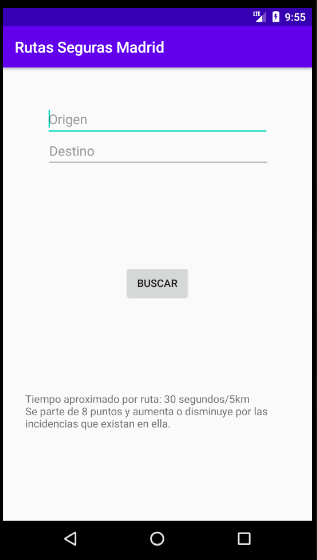
\includegraphics[angle=0, width=0.3\textwidth]{images/android/camposRuta.png}  
	
	\caption{Pagina Inicio Aplicación}
	\label{fig:diagramaOntologAccid}
\end{figure}


Cabe destacar que la clave que se está utilizando en este proyecto para la API de Google será restringida o cancelada un tiempo después de la finalización del proyecto. Debido a que no se va a comercializar y cualquiera podría reutilizar el código, se tendría que modificar dicho campo para utilizar una clave propia. Para que pueda mostrarse correctamente y probarse se ha decidido compartir durante cierto, aunque pasado un plazo se cancelará para evitar un mal uso de la misma.




Una vez se ha hecho la petición http se obtiene un fichero JSON con las características de la ruta. Para su tratamiento se han tenido de nuevo en cuenta las especificaciones y ejemplos proporcionados por en la web de Google \cite{apiDirections}.
De este fichero se obtienen los valores distancia y duración y todas y cada una de las coordenadas de la ruta. Para ello se ha creado una clase ``Coordinate`` cuyas propiedades son longitud y latitud. Para obtenerlas se recorre los distintos ``steps`` de los que está compuesto el JSON y se listan. El código detallado se encuentra en la ruta antes mencionada en el fichero MainActivity.java, en la función llamada getArrayCoordenadas.






Tras tener dicha lista de coordenadas, han de buscarse en la base de datos antes generada para obtener los identificadores de las vías por las que transcurre. Para ello se realizan peticiones SQL  a la base de datos con cada iteración de la lista anterior.
Al ser la ruta un conjunto de coordenadas separadas entre si por varios metros de distancia, es muy improbable que coincida exactamente con el punto almacenado (que sigue el mismo procedimiento). Es por ello que a la hora de buscar los puntos se ha aplicado un margen de error en varias fases. La primera de ellas de 15 metros, la segunda de 30, la tercera de 60... De modo que aun no siendo el punto exacto se pueda encontrar el más cercano a esa posición.
Al aplicar este margen de error podría darse el caso de que para un mismo punto existan varias calles sin ser necesariamente un cruce, en un radio de 15 metros puede haber varias coordenadas. Se genera por cada punto una lista de calles ``posibles`` y una lista de diferencias. Estas se calcularán con la suma del valor absoluto de las diferencias entre sus latitudes y longitudes (las de la coordenada de la ruta y la de la base de datos). Una vez se tengan estas listas, a ese punto le corresponderá la de menor diferencia, es decir, la más próxima.
El código detallado se encuentra en la ruta antes mencionada en el fichero PeticionesBBDD.java, en la función llamada getListaCallesPosibles.

Una vez finalizado este proceso para todas las coordenadas se tendrá una lista de calles, a la cual se le eliminarán los duplicados y de esta forma se podrá consultar las incidencias de las calles por las que la ruta transcurre.















\clearpage
\section{Cálculo de Seguridad de ruta}

Para el cálculo de la ``seguridad`` de la ruta, como se ha explicado anteriormente, no se ha seguido ninguna regla ni ningún procedimiento estadístico. Es por ello que no se consideran fiables las operaciones realizadas.
Sin embargo, si ha querido mostrarse la utilidad de los datos enlazados para una aplicación como esta y ha querido realizarse una aproximación ``subjetiva`` acorde a los datos existentes.

Para el cálculo se tendrán en cuenta los ciclocarriles, calles tranquilas y accidentes. A cada uno se le asignará un valor proporcional sobre la importancia que tienen en la ruta (3 para ciclocarriles, 2 para calles tranquilas y 5 para accidentes). En cada calle transitada se comprobará si tiene o no ciclocarril y si es ``calle tranquila``. En caso de serlo se sumará el modificador anterior dividido por el número de calles (de esta forma por ejemplo si todas las vías de la ruta son tranquilas, se sumarán al cálculo 2 puntos).
Para accidentes se han tenido en cuenta más variables como son la lesividad y el tipo de persona afectada. Primero se calculará la gravedad del siniestro (10 en caso de fallecimiento, 5 accidente grave y 1 leve), y posteriormente se multiplicará este valor por la ``importancia que le da el conductor de la bicicleta``. Esto último no es del todo correcto, pero se ha considerado que la persona que desea valorar la seguridad de la ruta da más importancia a su integridad (las bicicletas están más desprotegidas) que a la de otro conductor. Siguiendo esta línea se ha multiplicado la gravedad por 3 en caso de ser el conductor el afectado, por 2 en caso de ser un peatón o viajero, y por 1 en caso de ser otros.
Para el caso de accidentes se ha usado el mismo método que los anteriores con el modificador y la gravedad del accidente, aunque con ligeras modificaciones. Se ha puesto un valor tope (2 puntos) por calle, ya que vías con mucha longitud y muy peligrosas podrían reducir incluso los 10 puntos máximos que puede tener la ruta, por tanto debe restringirse.

Por último, es importante destacar que se parte de 8 puntos, es decir, que a partir de ahí se sumará o restará dependiendo de las incidencias detectadas. Se ha elegido esta cantidad inicial ya que permitía cierto margen para que las rutas pudiesen llegar a 10 en caso de haber muy pocos accidentes y que en zonas muy transcurridas no rozase constantemente el 0.

El código detallado se encuentra en la ruta antes mencionada en el fichero MainActivity.java, en la función llamada getNotaRuta y getGravedadAccidente.

Para obtener los datos necesarios para este proceso se ha hecho uso de Jena y de las consultas explicadas en el capítulo anterior. Dicho se encuentra en el fichero JenaRequest.java y contiene funciones con los valores de retorno antes mencionados.

Como se mencionó anteriormente se ha dado prioridad a mostrar las características de la ruta en vez de a únicamente el cálculo. Es por ello que en este proceso se ha detallado la puntuación que se ha sumado y restado por cada incidencia. De este modo cualquiera que lo use podría calcular la nota acorde a sus criterios.


En los siguientes ejemplos se observa cómo se han mostrado la nota y las incidencias de la ruta en la aplicación final desarrollada.


\clearpage
\begin{figure}[h]
	\centering
	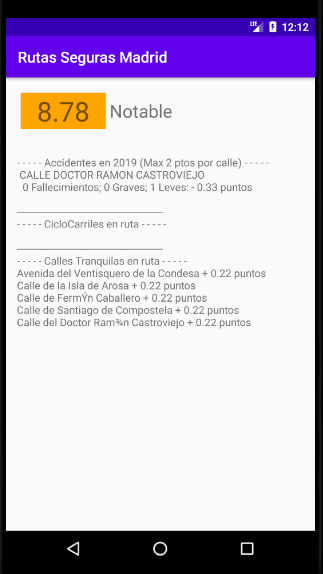
\includegraphics[angle=0, width=0.3\textwidth]{images/android/captura2.png}  
	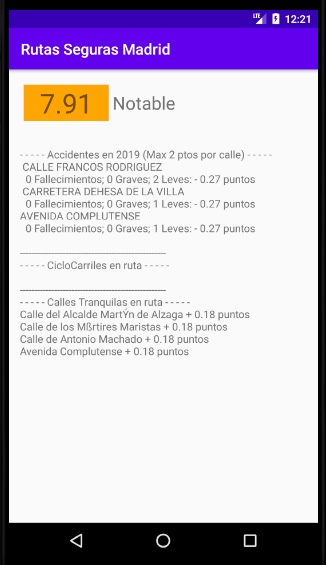
\includegraphics[angle=0, width=0.3\textwidth]{images/android/captura4.png} 
	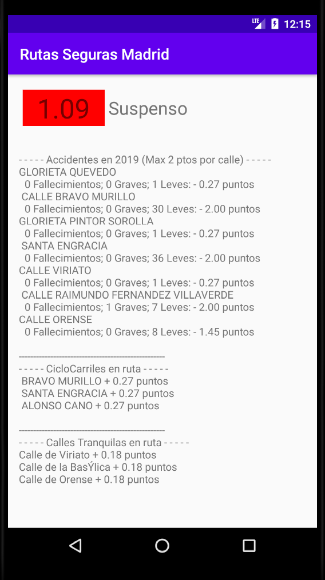
\includegraphics[angle=0, width=0.3\textwidth]{images/android/captura3.png}  
	
	\caption{Ejemplos de rutas}
	\label{fig:diagramaOntologAccid}
\end{figure}

En las capturas anteriores se muestran 3 rutas diferentes consultadas en Madrid.
La primera corresponde a la ruta entre Metro Mirasierra y Metro Peñagrande. Como se puede observa es bastante segura aun no teniendo ciclocarriles. Pocos accidentes han ocurrido en las calles por las que se transita y se han catalogado varias de ellas como tranquilas.
Lo mismo ocurre en la segunda captura, ruta entre Metro Valdezarza y E.T.S Agrónomos (Ciudad universitaria). En ésta han ocurrido unos pocos más accidentes leves, pero sigue considerándose segura.
Sin embargo, en la tercera imagen se muestra la ruta entre Bravo Murillo 1 y Calle de Orense 5. Se puede observar que hay ciclocarriles que aumentan en cierta medida la seguridad, sin embargo al ser una zona céntrica y con calles estrechas y muy concurridas, han ocurrido muchos accidentes, algunos de ellos graves, que han reducido drásticamente la seguridad de la misma. Cabe destacar en esta que la calle Raimundo Fernández Villaverde ha restado 2 puntos al cómputo general (que es el máximo permitido por calle).







%----------------------------------------------------------------------------------------------------------------------------------------------------------------------------------------------------------------------------------------------



\clearpage
\chapter{Resultados y conclusiones}

Resumen de resultados obtenidos en el TFG. Y conclusiones personales del estudiante sobre el trabajo realizado.



\begin{thebibliography}{99}

\bibitem{ciudadesbiertas_callejero}
\url{http://vocab.linkeddata.es/datosabiertos/def/urbanismo-infraestructuras/callejero/index-en.html}

\bibitem{schema_org}
\url{http://schema.org}

\bibitem{datosMadrid_accidentesDeBicicleta}
\url{https://datos.madrid.es/portal/site/egob/menuitem.c05c1f754a33a9fbe4b2e4b284f1a5a0/?vgnextoid=20f4a87ebb65b510VgnVCM1000001d4a900aRCRD&vgnextchannel=374512b9ace9f310VgnVCM100000171f5a0aRCRD&vgnextfmt=default}

\bibitem{datosMadrid_ciclocarriles}
\url{https://datos.madrid.es/portal/site/egob/menuitem.c05c1f754a33a9fbe4b2e4b284f1a5a0/?vgnextoid=435a7cd5de319410VgnVCM1000000b205a0aRCRD&vgnextchannel=374512b9ace9f310VgnVCM100000171f5a0aRCRD&vgnextfmt=default}

\bibitem{datosMadrid_callesTranquilas}
\url{https://datos.madrid.es/portal/site/egob/menuitem.c05c1f754a33a9fbe4b2e4b284f1a5a0/?vgnextoid=a320f5ac548f4410VgnVCM1000000b205a0aRCRD&vgnextchannel=374512b9ace9f310VgnVCM100000171f5a0aRCRD&vgnextfmt=default}


\bibitem{datosmadrid_callejero}
\url{https://datos.madrid.es/sites/v/index.jsp?vgnextoid=b3c41f3cf6a6c410VgnVCM2000000c205a0aRCRD&vgnextchannel=374512b9ace9f310VgnVCM100000171f5a0aRCRD}


\bibitem{openStreetMapCallesTranquilas}
\url{https://datos.madrid.es/egob/new/detalle/auxiliar/mapa.jsp?geoUrl=/egob/catalogo/205115-4-calles-tranquilas.kml}


\bibitem{datosIgnCalzada}
\url{https://datos.ign.es/def/btn100/index-es.html#calzada}

\bibitem{datosIgnMunicipios}
\url{https://www.ine.es/daco/daco42/codmun/codmunmapa.htm}

\bibitem{datosIgn_calzada}
\url{https://datos.ign.es/def/btn100/index-es.html#calzada}

\bibitem{datoabiertos_tipoVia}
\url{http://vocab.linkeddata.es/datosabiertos/def/urbanismo-infraestructuras/callejero/index-en.html#tipoVia}

\bibitem{datoabiertos_municipio}
\url{http://vocab.linkeddata.es/datosabiertos/def/sector-publico/territorio/index-en.html#Municipio}

\bibitem{datoabiertos_idVia}
\url{http://vocab.linkeddata.es/datosabiertos/def/urbanismo-infraestructuras/callejero/index-en.html#Via}

\bibitem{schema_gender}
\url{https://schema.org/gender}

\bibitem{schema_gender_explicacion_rango}
\url{https://lists.w3.org/Archives/Public/public-schemaorg/2019Oct/0013.html}

\bibitem{schema_typicalAgeRange}
\url{https://schema.org/typicalAgeRange}


\bibitem{datosabiertos_portal}
\url{http://vocab.linkeddata.es/datosabiertos/def/urbanismo-infraestructuras/callejero/index-en.html#Portal}


\bibitem{dc_identifier}
\url{https://www.dublincore.org/specifications/dublin-core/dcmi-terms/#http://purl.org/dc/terms/identifier}


\bibitem{ciudadesabiertas_catalogoVocabs}
\url{https://ciudadesabiertas.es/vocabularios/#CatálogoVocabularios}


\bibitem{datosabiertos_ayuntmadrid}
\url{https://datos.madrid.es/portal/site/egob}

\bibitem{mapa_callejero_klm}
\url{https://datos.madrid.es/egob/new/detalle/auxiliar/mapa.jsp?geoUrl=/egob/catalogo/205115-4-calles-tranquilas.kml}

\bibitem{calles_cambioNombre_elPais}
\url{https://elpais.com/ccaa/2017/04/28/madrid/1493369660_675682.html}


\end{thebibliography}

\addcontentsline{toc}{chapter}{Bibliografía}





%%-----------------------------------------------
%% Anexos
\appendix
\clearpage 
\addcontentsline{toc}{chapter}{Anexo}
\chapter*{Anexo}

\textbf{Calles añadidas al Callejero de Madrid}

Se ha seguido la lista proporcionada por El Pais \cite{calles_cambioNombre_elPais}.

\begin{tiny}
96200;CALLE;;BATALLA DE BELCHITE;BATALLA DE BELCHITE;2;1;15;2;22
\newline 917;PASEO;DEL;DOCTOR VALLEJO-NAJERA;DOCTOR VALLEJO-NÁJERA;2;1;61;2;56
\newline 356700;PLAZA;DE LOS;HERMANOS FALCO Y ALVAREZ;HERMANOS FALCÓ Y ÁLVAREZ;21;1;25;2;24
\newline 526000;PASEO;DE;MUÑOZ GRANDES;MUÑOZ GRANDES;11;1;53;2;64
\newline 329900;CALLE;DEL;GARCIA DE LA HERRANZ;GARCÍA DE LA HERRANZ;11;1;19;2;10
\newline 329700;CALLE;DEL;GENERAL FRANCO;GENERAL FRANCO;11;1;15;2;12
\newline 73600;PLAZA;;ARRIBA ESPAÑA;ARRIBA ESPAÑA;5;1;13;2;12
\newline 123600;CALLE;;CAIDOS DE LA DIVISION AZUL;CAÍDOS DE LA DIVISIÓN AZUL;5;1;15;2;28
\newline 82000;PLAZA;;AUNOS;AUNÓS;5;1;11;2;10
\newline 328950;CALLE;DE LA;POETA ANGELA FIGUERA;POETA ÁNGELA FIGUERA;7;1;41;2;22
\newline 329400;CALLE;DE;GENERAL DAVILA;GENERAL DÁVILA;7;1;15;2;12
\newline 419300;CALLE;DE;JUAN VIGON;JUAN VIGÓN;7;1;25;2;10
\newline 332950;CALLE;DEL;GENERAL RODRIGO;GENERAL RODRIGO;7;1;17;2;12
\newline 417850;PLAZA;;JUAN PUJOL;JUAN PUJOL;1;1;1;;
\newline 402600;CALLE;DE;JOSE LUIS DE ARRESE;JOSÉ LUIS DE ARRESE;15;1;91;2;66
\newline 48900;CALLE;DEL;ANGEL DEL ALCAZAR;ÁNGEL DEL ALCÁZAR;15;1;7;2;8
\newline 330300;CALLE;DEL;GENERAL KIRKPATRICK;GENERAL KIRKPATRICK;15;1;37;2;46
\newline 158300;PLAZA;DEL;CAUDILLO;CAUDILLO;8;1;5;2;4
\newline 609700;CALLE;;PRIMERO DE OCTUBRE;PRIMERO DE OCTUBRE;8;1;15;2;20
\newline 772400;PLAZA;DEL;VEINTIOCHO DE MARZO;VEINTIOCHO DE MARZO;8;1;11;2;10
\newline 137100;CALLE;DEL;CAPITAN CORTES;CAPITÁN CORTÉS;16;1;13;2;14
\newline 31000067;AVENIDA;DEL;ALCALDE CONDE MAYALDE;ALCALDE CONDE MAYALDE;8;;;;
\newline 28150;CALLE;DEL;ALGABEÑO;ALGABEÑO;16;1;125;2;192
\newline 329500;AVENIDA;DEL;GENERAL FANJUL;GENERAL FANJUL;10;1;185;2;144
\newline 331250;CALLE;DEL;GENERAL MILLAN ASTRAY;GENERAL MILLÁN ASTRAY;10;1;81;2;72
\newline 333250;CALLE;DEL;GENERAL SALIQUET;GENERAL SALIQUET;10;1;109;2;54
\newline 325200;CALLE;DE;GARCIA MORATO;GARCÍA MORATO;10;5;9;22;26
\newline 329850;CALLE;DEL;GENERAL GARCIA ESCAMEZ;GENERAL GARCÍA ESCÁMEZ;10;3;27;2;52
\newline 333000;CALLE;DEL;GENERAL ROMERO BASART;GENERAL ROMERO BASART;10;1;149;2;90
\newline 67700;AVENIDA;DEL;ARCO DE LA VICTORIA;ARCO DE LA VICTORIA;9;1;3;2;4
\newline 333200;PASEO;DEL;GENERAL SAGARDIA RAMOS;GENERAL SAGARDÍA RAMOS;9;1;7;2;24
\newline 31004081;GLORIETA;DE;RAMON GAYA;RAMÓN GAYA;9;;;;
\newline 144900;CALLE;DE;CARLOS RUIZ;CARLOS RUIZ;9;1;3;2;10
\newline 33025;CALLE;DEL;ALMIRANTE FRANCISCO MORENO;ALMIRANTE FRANCISCO MORENO;9;1;13;;
\newline 263650;PLAZA;DE;EMILIO JIMENEZ MILLAS;EMILIO JIMÉNEZ MILLAS;9;1;1;2;4
\newline 1887;CALLE;DEL;PUERTO DE LOS LEONES;PUERTO DE LOS LEONES;9;1;61;2;92
\newline 360800;CALLE;DE LOS;HEROES DEL ALCAZAR;HÉROES DEL ALCAZAR;13;;;2;12
\newline 166500;CALLE;DEL;CERRO DE GARABITAS;CERRO DE GARABITAS;13;1;17;2;12
\newline 220600;CALLE;DEL;CRUCERO BALEARES;CRUCERO BALEARES;13;1;25;2;16
\newline 338200;PLAZA;DEL;GOBERNADOR CARLOS RUIZ;GOBERNADOR CARLOS RUIZ;13;1;7;2;8
\newline 256300;CALLE;DE;EDUARDO AUNOS;EDUARDO AUNÓS;4;1;41;2;56
\newline 331500;PASAJE;DEL;GENERAL MOLA;GENERAL MOLA;4;1;9;2;6
\newline 357000;CALLE;DE LOS;HERMANOS GARCIA NOBLEJAS;HERMANOS GARCÍA NOBLEJAS;15;;;2;198
\newline 331800;CALLE;DEL;GENERAL ORGAZ;GENERAL ORGAZ;6;1;31;2;18
\newline 333900;CALLE;DEL;GENERAL VARELA;GENERAL VARELA;6;1;37;2;38
\newline 328800;CALLE;DEL;GENERAL ARANDA;GENERAL ARANDA;6;1;55;2;98
\newline 328900;ESCALINATA;DEL;GENERAL ARANDA;GENERAL ARANDA;6;;;;
\newline 466800;CALLE;DE;MANUEL SARRION;MANUEL SARRIÓN;6;1;13;2;12
\newline 137400;CALLE;;CAPITAN HAYA;CAPITAN HAYA;6;1;65;2;66
\newline 293200;PLAZA;DE;FERNANDEZ LADREDA;FERNÁNDEZ LADREDA;11;3;5;;
\newline 293200;PLAZA;DE;FERNANDEZ LADREDA;FERNÁNDEZ LADREDA;12;1;1;2;2
\end{tiny}




 
%%---------------------------------------------------------
\end{document}